% !TEX root = ex_article.tex
% SIAM Article Template
\documentclass[review,onefignum,onetabnum]{siamart171218}

% Information that is shared between the article and the supplement
% (title and author information, macros, packages, etc.) goes into
% ex_shared.tex. If there is no supplement, this file can be included
% directly.

\input{ex_shared}

% Optional PDF information
\ifpdf
\hypersetup{
  pdftitle={A robust shifted Schur-complement preconditioner for the
            implicit linearised Boussinesq equations},
  pdfauthor={Molin Han, Josh Hope-Collins, Colin J. Cotter}
}
\fi

% The next statement enables references to information in the
% supplement. See the xr-hyperref package for details.

%% Use \myexternaldocument on Overleaf
\myexternaldocument{ex_supplement}

% FundRef data to be entered by SIAM
%<funding-group>
%<award-group>
%<funding-source>
%<named-content content-type="funder-name"> 
%</named-content> 
%<named-content content-type="funder-identifier"> 
%</named-content>
%</funding-source>
%<award-id> </award-id>
%</award-group>
%</funding-group>

% \def\@a{\alpha}
% \def\@A{\Alpha}
% \def\@b{\beta}
% \def\@B{\Beta}
% \def\@g{\gamma}
% \def\@G{\Gamma}
% \def\@d{\delta}
% \def\@D{\Delta}
% \def\@e{\epsilon}
% \def\@E{\Epsilon}
% \def\:e{\varepsilon}
% \def\@z{\zeta}
% \def\@Z{\Zeta}
% \def\@t{\theta}
% \def\@T{\Theta}
% \def\@i{\iota}
% \def\@I{\Iota}
% \def\@k{\kappa}
% \def\@K{\Kappa}
% \def\@l{\lambda}
% \def\@L{\Lambda}
% \def\@s{\sigma}
% \def\@S{\Sigma}
% \def\@o{\omega}
% \def\@O{\Omega}

\newcommand{\red}[1]{\textcolor{red}{#1}}
\newcommand{\mh}[1]{\textcolor{cyan}{Molin says: #1}}
\newcommand{\colin}[1]{\textcolor{red}{Colin says: #1}}
\newcommand{\blue}[1]{\textcolor{blue}{#1}}
\newcommand{\review}[1]{\textcolor{blue}{\textbf{[Review:} #1\textbf{]}}}
\newcommand{\green}[1]{\textcolor{green}{#1}}
\newcommand{\orange}[1]{\textcolor{orange}{#1}}
% Better formatting for partial derivatives
\newcommand{\pder}[2]{\frac{\partial #1}{\partial #2}}
\newcommand{\TODO}[1][]{\textcolor{red}{[TODO: #1]}}
\newcommand{\opt}{}  % reserve the name (errors if already defined)
\DeclareUrlCommand\opt{\urlstyle{tt}}
\newcommand{\cjc}[1]{\textcolor{red}{\bfseries CJC says: #1}}

% Theorem-like environments.  These must be declared with the class's
% \newsiamthm / \newsiamremark rather than with a bare \newtheorem:
% siamart loads ntheorem together with cleveref, and an environment
% registered by \newtheorem after cleveref is loaded raises
% "Use of \cref@override@label@type doesn't match its definition"
% the first time it is used with an optional argument.
\numberwithin{theorem}{section}
\newsiamthm{thm}{Theorem}
\newsiamthm{theo}{Theorem}
\newsiamthm{cor}{Corollary}
\newsiamthm{coro}{Corollary}
\newsiamthm{conj}{Conjecture}
\newsiamthm{lem}{Lemma}
\newsiamthm{ques}{Question}
\newsiamthm{prop}{Proposition}
\newsiamthm{exa}{Example}
\newsiamthm{defi}{Definition}
\newsiamremark{rem}{Remark}

% Workaround for a cleveref/ntheorem/hyperref clash in this class: with
% hyperref loaded, cleveref redefines \refstepcounter@optarg to rewrite
% an existing \cref@currentlabel via \cref@override@label@type, but
% ntheorem does not leave one in the expected [type][num][prefix] form,
% so the FIRST theorem carrying an optional argument aborts the run with
% "Use of \cref@override@label@type doesn't match its definition".
% Restoring cleveref's non-hyperref definition, which builds the label
% from scratch instead of overriding one, fixes it. Without this, no
% \begin{thm}[Named theorem] anywhere in the document will compile.
\makeatletter
\AtBeginDocument{%
  \def\refstepcounter@optarg[#1]#2{%
    \cref@old@refstepcounter{#2}%
    \cref@constructprefix{#2}{\cref@result}%
    \@ifundefined{cref@#1@alias}%
      {\def\@tempa{#1}}%
      {\def\@tempa{\csname cref@#1@alias\endcsname}}%
    \protected@edef\cref@currentlabel{%
      [\@tempa][\arabic{#2}][\cref@result]%
      \csname p@#2\endcsname\csname the#2\endcsname}}%
}
\makeatother
\usepackage{amssymb}
\usepackage{booktabs}
\usepackage{tikz}
\usetikzlibrary{cd}
\usetikzlibrary{calc, positioning, trees, plotmarks}
\usetikzlibrary{shapes, shapes.geometric, decorations.pathreplacing, decorations.markings}
\usetikzlibrary{arrows, arrows.meta, chains, fit, backgrounds, scopes}
% https://tex.stackexchange.com/questions/27171/padded-boundary-of-convex-hull
\newcommand{\convexpath}[2]{
  [
  create hullcoords/.code={
    \global\edef\namelist{#1}
    \foreach [count=\counter] \nodename in \namelist {
      \global\edef\numberofnodes{\counter}
      \coordinate (hullcoord\counter) at (\nodename);
    }
    \coordinate (hullcoord0) at (hullcoord\numberofnodes);
    \pgfmathtruncatemacro\lastnumber{\numberofnodes+1}
    \coordinate (hullcoord\lastnumber) at (hullcoord1);
  },
  create hullcoords
  ]
  ($(hullcoord1)!#2!-90:(hullcoord0)$)
  \foreach [
  evaluate=\currentnode as \previousnode using \currentnode-1,
  evaluate=\currentnode as \nextnode using \currentnode+1
  ] \currentnode in {1,...,\numberofnodes} {
    let \p1 = ($(hullcoord\currentnode) - (hullcoord\previousnode)$),
    \n1 = {atan2(\y1,\x1) + 90},
    \p2 = ($(hullcoord\nextnode) - (hullcoord\currentnode)$),
    \n2 = {atan2(\y2,\x2) + 90},
    \n{delta} = {Mod(\n2-\n1,360) - 360}
    in
    {arc [start angle=\n1, delta angle=\n{delta}, radius=#2]}
    -- ($(hullcoord\nextnode)!#2!-90:(hullcoord\currentnode)$)
  }
}

\usetikzlibrary{shapes.geometric, arrows}

\tikzstyle{startstop} = [rectangle, rounded corners, minimum width=3cm, minimum height=1cm,text centered, draw=blue, fill=blue!10]
\tikzstyle{process} = [rectangle, minimum width=3cm, minimum height=1cm, text centered, draw=blue, fill=blue!10]
\tikzstyle{decision} = [diamond, minimum width=3cm, minimum height=1cm, text centered, draw=blue, fill=blue!10]
\tikzstyle{arrow} = [thick,->,>=stealth]
\tikzstyle{note} = [rectangle, draw=gray!60, fill=gray!20, minimum width=1cm, minimum height=0.6cm, font=\scriptsize]


% Bibliography
\usepackage[numbers, comma, square, sort&compress]{natbib}
% \bibliographystyle{abbrvunsrtnat.bst}
% \bibliographystyle{alpha}



\begin{document}

\maketitle

% REQUIRED
\begin{abstract}
  Implicit time integration of the incompressible Boussinesq equations
  removes the gravity-wave CFL restriction that limits explicit ocean
  models, at the cost of solving a saddle-point system coupling
  velocity, buoyancy and pressure at every step.  On the thin domains
  characteristic of ocean basins this system is hard to precondition:
  the $H(\mathrm{div})$ velocity block is poorly conditioned on
  anisotropic meshes, and the gravity-wave coupling makes the pressure
  Schur complement sensitive to the time step.  We propose and analyse
  a preconditioner built from a shifted problem in which the pressure
  equation is augmented by a small multiple $\delta$ of the pressure
  mass matrix.  The shift makes the pressure block invertible in
  isolation, permitting an exact Schur-complement elimination of the
  pressure and reducing each solve to a velocity--buoyancy block with a
  grad--div augmentation, treated by multigrid with a vertical
  column-patch smoother.  Our main result bounds the spectral distance
  between the shifted and unshifted operators explicitly in terms of
  $\delta$, the time step, the buoyancy frequency and the aspect ratio,
  in a norm weighted by the stratification operator; bounds are given
  with and without the assumption that the velocity block is symmetric,
  and they agree to leading order.  The inf--sup constant is shown to
  be exactly independent of the aspect ratio throughout the thin-domain
  regime, so the preconditioner is uniform precisely in the limit where
  standard approaches degrade, and the analysis predicts a two-regime
  scaling for $\delta$ whose cross-over is governed jointly by the
  aspect ratio and the stratification rather than by the time step
  alone.  Numerical experiments confirm robustness in mesh resolution,
  aspect ratio and shift parameter for both the linear and the
  nonlinear problem, and a terrain-following flow-over-a-ridge test
  case demonstrates the solver on a deformed geometry.
\end{abstract}

% REQUIRED
\begin{keywords}
  Preconditioning,
  Boussinesq System, Compatible Finite Elements, Multigrid,
  Parameter Robustness, Implicit Time Stepping.
\end{keywords}

% REQUIRED
\begin{AMS}
  65N30
  (finite element methods for BVPs), 65F08 (preconditioners for linear
  systems), 65N55 (multigrid methods), 76D07 (Stokes and related problems).
\end{AMS}

\section{Introduction}
\label{sec:intro}
Numerical models of the ocean must integrate the governing equations over timescales far longer than the periods of the fastest waves the equations support. 
The incompressible Boussinesq system, which forms the dynamical core of many ocean models, admits 
internal gravity waves whose frequencies reach the buoyancy frequency $N$. 
In the small aspect ratio regime characteristic of 
ocean basins, where the horizontal extent exceeds the vertical extent by three or more orders of magnitude, these waves propagate quickly relative to the slow circulation that is the quantity of 
physical interest. 
An explicit time integration of the system is restricted by the Courant--Friedrichs--Lewy (CFL) condition tied to the gravity-wave speed, which forces time steps far smaller than accuracy alone would require.
Implicit time integration removes this restriction, at the cost of solving a large linear system at every 
step. 
The efficiency of an implicit ocean model is therefore
determined by the efficiency of the linear solver, and the design of a solver that remains effective and robust as the time step, the mesh resolution, and the aspect ratio vary is the problem addressed in this report.
Operational ocean models have long avoided a fully implicit treatment of the fast waves by splitting the dynamics to isolate computationally stiff fast components. The classical strategy is barotropic--baroclinic (mode) splitting, in which the depth-averaged barotropic mode is stepped implicitly or sub-cycled at a small time step~\cite{dukowiczSmith1994} while the residual baroclinic mode is integrated at the dynamical time step; this underpins models such as FESOM~\cite{danilov2017fesom2} and MITgcm~\cite{marshall1997mitgcm}. An alternative is the split-explicit scheme used in MPAS-Ocean~\cite{kang2021mpas} and ROMS~\cite{shchepetkin2005roms}, in which the fast barotropic equations are sub-cycled within each slow step without a formal mode decomposition. Each of these approaches removes the gravity-wave CFL restriction from the fast component at comparatively low cost, since the barotropic or fast sub-problem has far fewer degrees of freedom than the full system, and they remain the standard approach in large-scale ocean circulation models. The splitting is, however, an approximation: it presumes a clean scale separation between the barotropic and baroclinic modes that is not always present, for instance in strongly stratified or strongly rotating regimes, or when internal gravity waves of frequency comparable to the time step of interest are themselves part of the dynamics being resolved. A fully implicit treatment of the system avoids this splitting error and remains accurate across the full range of wave frequencies the discretisation supports, at the cost that every time step now requires the solution of a saddle-point linear system coupling all three fields, rather than a sequence of smaller barotropic and baroclinic solves. The construction of a linear solver that is robust enough to make this fully implicit alternative competitive is the motivation for the remainder of the report.

For the purposes of this report we study the Boussinesq equations
linearised about a state of rest, since the linearisation makes the
theory tractable. The approach is, however, designed with the full
nonlinear equations in view: there, the preconditioner is used for the
iterative solution of the Jacobian system arising at each step of a
Newton method, a setting exercised directly by the nonlinear
experiments of Section~\ref{sec:numerical}.
We work with a compatible finite element discretisation of the linearised nonhydrostatic Boussinesq equations. 
Compatible finite element methods preserve discrete analogues of the differential structure of the continuous equations, 
and have become a standard tool in geophysical fluid 
dynamics~\cite{cotter2023compatible, cotterShipton2012}. 
The discretisation places velocity in an $H(\mathrm{div})$-conforming 
Raviart--Thomas space, pressure in a discontinuous space, and buoyancy in a tensor-product space chosen to avoid the spurious modes that arise from an incompatible pairing~\cite{natale2016compatible, melvin2018choice}. 
The implicit time discretisation produces, at each step, a saddle-point linear system coupling velocity, buoyancy, and pressure. 
Two features of this system make it difficult to precondition. The velocity block is an 
$H(\mathrm{div})$ mass-type operator whose conditioning degrades on the anisotropic meshes that small aspect ratios demand, a difficulty 
already identified for the related elliptic problem on thin domains~\cite{cotterPain2010}.
The saddle-point structure, with its 
zero pressure block, prevents a direct block factorisation and requires a Schur-complement treatment that the gravity-wave coupling renders sensitive to the time step.

The preconditioner developed here is built on operator preconditioning, in which a discrete operator is preconditioned by a norm-equivalent operator derived from the mapping properties of the continuous problem~\cite{mardalWinther2011, kirby2010}. 
We introduce a shifted perturbation of the saddle-point system that augments the pressure 
equation with a small multiple of the pressure mass matrix. 
The shift makes the pressure block invertible in isolation, which permits an exact Schur-complement elimination of the pressure and 
reduces the solve to a velocity-buoyancy block augmented by a grad-div term. 
The size of the shift controls the spectral distance between the shifted operator and the original one, and the central theoretical result of the report is a bound on this distance with explicit dependence on the time step, the buoyancy frequency, and the aspect ratio. 
The bound is obtained by reducing the shifted problem to a perturbed mixed problem and identifying the relevant inf-sup constant.
A consequence of the bound is that the inf--sup constant is exactly independent of the aspect ratio throughout the thin domain regime, so the preconditioner is robust precisely in the limit where standard approaches degrade. 
The bound also predicts the scaling of the shift parameter with the time step, and this prediction is recovered in the numerical experiments.

The velocity-buoyancy block that remains after the Schur-complement reduction is solved by a multigrid method with a patch-based line smoother. 
The smoother relaxes over overlapping patches of vertical columns of the extruded mesh, which captures the strong vertical coupling induced by the small aspect ratio. 
This patch structure differs from the monolithic 
patch smoothers applied directly to the full saddle-point system~\cite{farrellMitchellWechsung2019}, in which each patch contains velocity and pressure degrees of freedom. 
Monolithic patches are robust but carry a high cost per application because of their size. 
The Schur-complement reduction used here yields smaller patches that contain only velocity-buoyancy degrees of freedom, and the efficient patch assembly available in Firedrake~\cite{firedrake2016} makes the resulting solver practical. 
We report timings for the preconditioner application and examine the effect of a reordering of the patch subproblems on the cost of the local factorisations.

The contribution of the report is a shifted Schur-complement 
preconditioner for the implicit linearised Boussinesq equations that is robust in the time step, the mesh resolution, and the aspect ratio, together with an analysis that establishes this robustness and predicts the choice of the shift parameter. 
The work is a step towards an efficient implicit solver for ocean models, and is restricted to the linearised equations so that the parameter robustness of the linear solver can be studied in isolation from the 
outer nonlinear iteration. 
The linearised system is the inner solve in any Newton or Picard iteration for the full nonlinear problem, so 
its robust solution is a prerequisite for an efficient nonlinear solver.

Shifting an indefinite or singular operator to make it more amenable to a direct or iterative inner solve, and then using the shifted operator as a preconditioner for the original problem, is a strategy with substantial precedent outside the saddle-point setting considered here. The closest analogue is the shifted-Laplacian preconditioner for the Helmholtz equation, in which the indefinite Helmholtz operator is preconditioned by a complex-shifted variant that is definite and therefore amenable to multigrid~\cite{erlangga2004class, erlangga2006novel}; the shift parameter there plays a role directly analogous to $\delta$ here, trading proximity to the original operator against the conditioning of the auxiliary problem, and a substantial body of work has developed sharp estimates for this trade-off and for sweeping and domain-decomposition variants of the idea~\cite{ganderZhang2019helmholtz}. The shifted-Schur preconditioner developed below is the corresponding construction for the saddle-point structure of the Boussinesq system: the shift acts on the zero pressure block rather than on an indefinite term, but the underlying mechanism, a small perturbation that restores well-posedness of an auxiliary problem at a controllable spectral cost, is the same.

The rest of the report is organised as follows. 
Section~\ref{sec:main} describes the governing equations, the compatible finite element discretisation, and the implicit time discretisation. 
Section~\ref{sec:precond} constructs the shifted 
Schur-complement preconditioner and the patch-based multigrid solver. 
Section~\ref{sec:theory} establishes the convergence bound and the asymptotic scaling of the shift parameter. 
Section~\ref{sec:numerical} reports the numerical experiments, 
confirming parameter robustness and the predicted shift-parameter 
scaling. Section~\ref{sec:conclusions} concludes, and
Section~\ref{sec:future} sets out the directions for future work.
Implementation details of the time stepper and the solver
configuration are collected in the appendices.

\section{Governing Equations and Discretisations}
\label{sec:main}
\subsection{Governing equations}
\label{sec:governing}

We model large-scale oceanic flows using the incompressible Boussinesq
system, linearised about a hydrostatic background state with linear
stratification. The linearised system and its weak formulation below
are posed on a general three-dimensional domain, since this is the
setting in which the preconditioner of Section~\ref{sec:precond} and
the theory of Section~\ref{sec:theory} are developed; the
two-dimensional vertical slice in the $x$--$z$ plane used for the
compatible finite element discretisation and the numerical experiments
of this report is introduced as a specialisation at the end of this
section.

We begin from the three-dimensional incompressible Boussinesq system,
consisting of the momentum equation,
\begin{align}
    \pder{\vec{u}}{t} + (\vec{u} \cdot \nabla) \vec{u}
    + 2 \Omega \times \vec{u} + \nabla p - b \hat{k} = 0,
    \label{eq:momentum}
\end{align}
the incompressibility constraint,
\begin{align}
    \nabla \cdot \vec{u} = 0,
    \label{eq:continuity}
\end{align}
and the transport equation for buoyancy,
\begin{align}
    \pder{b}{t} + \vec{u} \cdot \nabla b = 0,
    \label{eq:transport}
\end{align}
where $\vec{u} = (u, v, w)$ is the three-dimensional velocity vector,
$p$ is the pressure, $b$ is the buoyancy, and $2\Omega = (0, 0, f)$
with $f$ the constant Coriolis parameter.
In general $f$ varies with latitude, neither
the discretisation nor the preconditioner relies on $f$ being
constant, since the Coriolis term enters only through the pointwise
skew operator $\vec{u} \mapsto f\,\hat{k}\times\vec{u}$.

To linearise about a hydrostatic background state, we decompose each
variable into a steady background state and a perturbation,
\begin{align}
    b = \bar{b} + b', \quad
    \vec{u} = \bar{\vec{u}} + \vec{u}', \quad
    p = \bar{p} + p',
\end{align}
with linear stratification $\bar{b}(z) = N^2(z) z$, where $N(z)$ is the
buoyancy frequency that may depend on depth, and no background flow 
$\bar{\vec{u}} = (0, 0, 0)$ for simplicity. The background pressure $\bar{p}$ is 
determined up to a constant by the hydrostatic balance
$\nabla \bar{p} - \bar{b}\hat{k} = 0$. Substituting the decomposition
into~\eqref{eq:momentum}--\eqref{eq:transport} and discarding terms
quadratic in the perturbations yields the linearised Boussinesq
equations,
\begin{align}
    \pder{\vec{u}'}{t} + 2 \Omega \times \vec{u}'
    + \nabla p' - b' \hat{k} &= 0,
    \label{eq:lin-mom}\\
    \pder{b'}{t} + N^2 w' &= 0,
    \label{eq:lin-buoy}\\
    \nabla \cdot \vec{u}' &= 0,
    \label{eq:lin-div}
\end{align}
posed on $\Omega \times [0, T]$, where
$\Omega = [0, L_x] \times [0, L_y] \times [0, L_z] \subset \mathbb{R}^3$
is a rectangular box domain with horizontal extents $L_x, L_y > 0$ and
depth $L_z > 0$. 
The domain is periodic in the two horizontal directions
$x$ and $y$ and bounded above and below by rigid lids. 
This specific choice of geometry and boundary conditions is an
assumption made for the theoretical results of
Section~\ref{sec:theory} rather than a limitation of the method. In
particular, free-slip boundary conditions in the horizontal
directions can be handled in the same way.
The
three-dimensional aspect ratios $\varepsilon_x = L_z / L_x$ and
$\varepsilon_y = L_z / L_y$ measure the shallowness of the domain; in
ocean basins, both are typically of order $10^{-3}$ or
smaller. The boundary conditions are the no-flux condition
$\vec{u}' \cdot \hat{n} = 0$ on the top and bottom boundaries
$\partial\Omega_{\mathrm{top}} \cup \partial\Omega_{\mathrm{bot}}$. We have used the
linear stratification $\bar{b}(z) = N^2 z$ to
write~$w' \, \partial_z \bar{b} = N^2 w'$ in~\eqref{eq:lin-buoy}.

To prepare for the compatible finite element discretisation of Section~\ref{sec:discretisation} and the preconditioner and theory of
Sections~\ref{sec:precond} and~\ref{sec:theory}, we cast the linearised
system~\eqref{eq:lin-mom}--\eqref{eq:lin-div} in weak form, on the
general three-dimensional domain $\Omega$ introduced above.
Multiplying the equation by test functions, integrating over
$\Omega$, and integrating the pressure-gradient term by parts, we
obtain the following weak form: find
$\vec{u}'(t) \in \mathring{H}(\mathrm{div})$,
$b'(t) \in L^2$,
$p'(t) \in \mathring{L}^2(\Omega)$ such that for all
$(\vec{w}, q, \phi) \in
\mathring{H}(\mathrm{div}) \times \mathbb{W}^\theta \times \mathring{L}^2(\Omega)$,
\begin{subequations}\label{eq:weak}
\begin{align}
    \left\langle \vec{w},\, \pder{\vec{u}'}{t} \right\rangle
    + \left\langle \vec{w},\, 2\Omega \times \vec{u}' \right\rangle
    - \left\langle \nabla \cdot \vec{w},\, p' \right\rangle
    - \left\langle \vec{w},\, b'\hat{k} \right\rangle &= 0,
    \label{eq:weak-mom}\\
    \left\langle q,\, \pder{b'}{t} \right\rangle
    + \left\langle q,\, N^2 \vec{u}' \cdot \hat{k} \right\rangle &= 0,
    \label{eq:weak-buoy}\\
    \left\langle \phi,\, \nabla \cdot \vec{u}' \right\rangle &= 0,
    \label{eq:weak-div}
\end{align}
\end{subequations}
where $\langle \cdot, \cdot \rangle$ denotes the $L^2(\Omega)$ inner
product, applied componentwise where appropriate, and
\begin{align}
    \mathring{H}(\mathrm{div}) =
    \left\{
    \vec{w} \in H(\mathrm{div}; \Omega) :
    \vec{w} \cdot \hat{n} = 0
    \text{ on }
    \partial\Omega_{\mathrm{top}} \cup \partial\Omega_{\mathrm{bot}}
    \right\}
\end{align}
encodes the no-flux boundary condition as an essential condition.


We define the mean-zero pressure space
\begin{align}
    \mathring{L}^2(\Omega) :=
    \Bigl\{ p \in L^2(\Omega) : \textstyle\int_\Omega p \,\mathrm{d}x = 0 \Bigr\}.
    \label{eq:L2ring}
\end{align}
The restriction $p'(t) \in \mathring{L}^2(\Omega)$ is the correct function
space for the pressure: since $\nabla \cdot \vec{w}$ has zero mean for
every $\vec{w} \in \mathring{H}(\mathrm{div})$ on a domain with no
inflow or outflow boundary, the divergence
equation~\eqref{eq:weak-div} only constrains $p'$ up to a global
additive constant. Imposing $p' \in \mathring{L}^2(\Omega)$ removes this
redundancy and renders the variational
problem~\eqref{eq:weak}--\eqref{eq:weak-div} uniquely solvable. This
single global mean-zero constraint has no localised basis representation
and is the source of the saddle-point structure discussed in
Section~\ref{sec:precond} below; we return to how it is affected by the
slice reduction that follows, and by the passage to the discrete setting,
once the block structure of the discrete system has been introduced.

For the numerical experiments of this report we
specialise the three-dimensional system above to a two-dimensional
vertical slice in the $x$--$z$ plane as a simplified model problem. In the vertical slice model, we
restrict the spatial dependence of the perturbed variables to the
$x$--$z$ plane while retaining all three Cartesian components of the
velocity field. With $\partial_y \equiv 0$ on every perturbed
variable, the gradient and divergence operators
in~\eqref{eq:lin-mom}--\eqref{eq:lin-div} act only in $x$ and $z$,
\begin{align}
    \nabla \phi
    = \left( \pder{\phi}{x},\, 0,\, \pder{\phi}{z} \right), \qquad
    \nabla \cdot \vec{u}' = \pder{u'}{x} + \pder{w'}{z},
\end{align}
and, reusing the symbol $\Omega$ for the remainder of the report to 
denote this two-dimensional slice domain, we take
$\Omega = [0, L_x] \times [0, L_z] \subset \mathbb{R}^2$ with aspect
ratio 
\begin{align}
    \varepsilon = \frac{L_z}{L_x},
    \label{eq:aspect-ratio}
\end{align}
which coincides with $\varepsilon_x$ from the three-dimensional domain
above. In the oceanic regime motivating this work, $\varepsilon$ is
typically of order $10^{-3}$ or smaller.
The slice form of the linearised
system~\eqref{eq:lin-mom}--\eqref{eq:lin-div} reads
\begin{subequations}\label{eq:slice}
\begin{align}
    \pder{u'}{t} - f v' + \pder{p'}{x}  &= 0, \label{eq:slice-u}\\
    \pder{v'}{t} + f u'                  &= 0, \label{eq:slice-v}\\
    \pder{w'}{t} + \pder{p'}{z} - b'     &= 0, \label{eq:slice-w}\\
    \pder{b'}{t} + N^2 w'                &= 0, \label{eq:slice-b}\\
    \pder{u'}{x} + \pder{w'}{z}          &= 0, \label{eq:slice-div}
\end{align}
\end{subequations}
on $\Omega \times [0, T]$, with the boundary and initial conditions
inherited from the three-dimensional system above. The weak
form~\eqref{eq:weak}--\eqref{eq:weak-div} specialises directly to the
slice: $H(\mathrm{div}; \Omega)$, $\mathbb{W}^\theta$, and $L^2(\Omega)$
are simply taken on the two-dimensional slice domain.

The system~\eqref{eq:slice} exposes the two coupled wave processes
that drive the dynamics and motivate the implicit time stepping used
in this report. Equations~\eqref{eq:slice-w} and~\eqref{eq:slice-b},
together with the divergence constraint~\eqref{eq:slice-div}, support
internal gravity waves with frequency bounded above by the buoyancy
frequency $N$, while \eqref{eq:slice-u}--\eqref{eq:slice-v} carry
inertial oscillations at the Coriolis frequency $f$. In oceanic
applications, the timescales of interest are typically those of the
slow, large-scale circulation, while the fastest internal gravity
waves are several orders of magnitude faster. Resolving these waves
explicitly imposes a severe CFL restriction that is decoupled from any
accuracy requirement on the dynamics one actually wishes to track.
Moreover, ocean basins exhibit aspect ratios $\varepsilon$
that are typically much smaller than their atmospheric counterparts,
which sharpens the anisotropy of the discrete operator and makes
solver robustness in $\varepsilon$ a practical requirement.

\subsection{Finite element discretisation}
\label{sec:discretisation}

We discretise the weak form~\eqref{eq:weak} in space using a compatible
finite element triple on an extruded quadrilateral mesh, following the
framework developed in~\cite{cotter2023compatible}. The temporal
discretisation, described in Section~\ref{sec:time}, uses a fully
implicit midpoint rule.

In the three-dimensional setting, the domain
$\Omega = [0,L_x]\times[0,L_y]\times[0,L_z]$ is discretised by an
extruded mesh: a two-dimensional structured horizontal base mesh is
extruded vertically into $N_z$ layers, producing a hexahedral mesh
whose cells inherit the anisotropy of the small aspect ratios
$\varepsilon_x, \varepsilon_y$. The tensor-product structure of the
extrusion carries over directly to the finite element spaces,
facilitating compatible discretisations in three dimensions.
For the two-dimensional vertical-slice experiments of this report, the
slice domain $\Omega = [0, L_x] \times [0, L_z]$ is discretised by
the corresponding lower-dimensional construction: a one-dimensional
base mesh of $N_x$ intervals in the horizontal direction is extruded
vertically into $N_z$ layers, producing a structured quadrilateral mesh
on $\Omega$ with cell widths $\Delta x = L_x / N_x$ and
$\Delta z = L_z / N_z$. The extruded construction produces the strongly
anisotropic cells associated with small aspect ratios
$\varepsilon = L_z / L_x$ without the mesh-generation difficulties of
unstructured meshes in thin domains.  It also brings two practical
advantages that the solver of Section~\ref{sec:precond} relies on.
The tensor-product finite element spaces the extrusion induces are
generated symbolically from their horizontal and vertical
factors~\cite{ExtrudedMesh_McRae_2016}, so that the triple below is
assembled without hand-coding the product elements; and the degrees of
freedom are numbered so as to exploit the fixed column structure of the
mesh~\cite{ExtrudedMesh_Bercea_2016}, which makes the data belonging to
a vertical column contiguous.  The latter is what allows the
column-patch smoother of Section~\ref{sec:inner-solvers} to be
assembled and applied as a local operation.

We adopt the compatible finite element triple
of~\cite{natale2016compatible, melvin2018choice}, as surveyed in~\cite{cotter2023compatible}. For polynomial degree $k \geq 1$, the
discrete spaces for velocity, buoyancy and pressure on the extruded
quadrilateral mesh are
\begin{align}
    H_h(\mathrm{div}) = \mathrm{RT}_k, \qquad
    \mathbb{W}_h^\theta = \mathrm{DG}_{k-1} \otimes \mathrm{CG}_k, \qquad
    L_h^2 = \mathrm{DG}_{k-1},
    \label{eq:fe-triple}
\end{align}
where $H_h(\mathrm{div}) \subset H(\mathrm{div}; \Omega)$ is the
Raviart--Thomas space, $L_h^2 \subset L^2(\Omega)$ is the fully
discontinuous pressure space with mean-zero subspace
$\mathring{L}_h^2 = \{p_h \in L_h^2 : \int_\Omega p_h \,\mathrm{d}x = 0\}$,
and $\mathbb{W}_h^\theta$ is the
tensor-product buoyancy space, discontinuous in the horizontal
direction and continuous in the vertical. The vertical continuity of
$\mathbb{W}_h^\theta$ aligns the buoyancy degrees of freedom with the
vertical component of $H_h(\mathrm{div})$ on horizontal facets,
eliminating the spurious modes that would arise from a fully
discontinuous buoyancy space; we refer
to~\cite{melvin2018choice} and to~\cite[Section~5]{cotter2023compatible} for a detailed discussion.

The no-flux boundary condition is imposed as an essential condition
on $H_h(\mathrm{div})$. We write
\begin{align}
    \mathring{H}_h(\mathrm{div}) =
    \left\{
    \vec{w} \in H_h(\mathrm{div}) :
    \vec{w} \cdot \hat{n} = 0
    \text{ on }
    \partial\Omega_{\mathrm{top}} \cup \partial\Omega_{\mathrm{bot}}
    \right\}.
\end{align}
Periodicity in the horizontal direction is built into the base mesh
and is inherited by all three spaces. In the numerical experiments of
Section~\ref{sec:numerical} we take $k = 2$, giving the second-order
$\mathrm{RT}_2 \otimes \mathbb{W}_h^\theta \otimes \mathrm{DG}_1$
triple.

The semi-discrete problem reads: find
$\vec{u}'_h(t) \in \mathring{H}_h(\mathrm{div})$,
$b'_h(t) \in \mathbb{W}_h^\theta$,
$p'_h(t) \in \mathring{L_h^2}$ such that for all 
$(\vec{w}, q, \phi) \in
\mathring{H}_h(\mathrm{div}) \times \mathbb{W}_h^\theta \times \mathring{L_h^2}$,
\begin{subequations}\label{eq:semi-discrete}
\begin{align}
    \left\langle \vec{w},\, \pder{\vec{u}'_h}{t} \right\rangle
    + \left\langle \vec{w},\, 2\Omega \times \vec{u}'_h \right\rangle
    - \left\langle \nabla \cdot \vec{w},\, p'_h \right\rangle
    - \left\langle \vec{w},\, b'_h\hat{k} \right\rangle &= 0,
    \label{eq:semi-discrete-mom}\\
    \left\langle q,\, \pder{b'_h}{t} \right\rangle
    + \left\langle q,\, N^2 \vec{u}'_h \cdot \hat{k} \right\rangle &= 0,
    \label{eq:semi-discrete-buoy}\\
    \left\langle \phi,\, \nabla \cdot \vec{u}'_h \right\rangle &= 0.
    \label{eq:semi-discrete-div}
\end{align}
\end{subequations}
The compatibility of the triple~\eqref{eq:fe-triple} ensures that the
divergence operator maps $H_h(\mathrm{div})$ surjectively onto
$L_h^2$, so the discrete inf--sup condition holds and the divergence
constraint~\eqref{eq:semi-discrete-div} is discretised consistently.
This compatibility is the structural property exploited by the
preconditioner constructed in Section~\ref{sec:precond}.

\subsection{Time discretisation}
\label{sec:time}
The semi-discrete system~\eqref{eq:semi-discrete} is integrated in
time using a fully implicit midpoint rule.
Writing $\bar{(\cdot)} := \tfrac{1}{2}\bigl( (\cdot)^{n+1} + (\cdot)^n \bigr)$
for the midpoint average, the fully discrete update from $t_n$ to
$t_{n+1} = t_n + \Delta t$ reads: find
$(\vec{u}'^{\,n+1}_h, b'^{\,n+1}_h, p'^{\,n+1}_h) \in
\mathring{H}_h(\mathrm{div}) \times \mathbb{W}_h^\theta \times \mathring{L}_h^2$
such that 
\begin{subequations}\label{eq:fully-discrete}
\begin{align}
    \left\langle \vec{w},\, \vec{u}'^{\,n+1}_h - \vec{u}'^{\,n}_h \right\rangle
    + \Delta t \left\langle \vec{w},\, 2\Omega \times \bar{\vec{u}}'_h \right\rangle
    - \Delta t \left\langle \nabla \cdot \vec{w},\, p'^{\,n+1}_h \right\rangle
    \nonumber\\
    {} - \Delta t \left\langle \vec{w},\, \bar{b}'_h \hat{k} \right\rangle
    &= 0,
    \label{eq:fully-discrete-mom}\\
    \left\langle q,\, b'^{\,n+1}_h - b'^{\,n}_h \right\rangle
    + \Delta t \left\langle q,\, N^2 \bar{\vec{u}}'_h\cdot \hat{k} \right\rangle
    &= 0,
    \label{eq:fully-discrete-buoy}\\
    \left\langle \phi,\, \nabla \cdot \vec{u}'^{\,n+1}_h \right\rangle
    &= 0,
    \label{eq:fully-discrete-div}
\end{align}
\end{subequations}
for all
$(\vec{w}, q, \phi) \in
\mathring{H}_h(\mathrm{div}) \times \mathbb{W}_h^\theta \times \mathring{L}_h^2$.
The system~\eqref{eq:fully-discrete} is the linear saddle-point
problem whose block structure is analysed and preconditioned in
Sections~\ref{sec:precond} and~\ref{sec:theory}.

\section{Preconditioning strategy}
\label{sec:precond}
The fully discrete system~\eqref{eq:fully-discrete} is a linear
saddle-point problem at each time step. In this section we construct
the preconditioner that is the main contribution of the report. The
construction has three structural ingredients: a shifted perturbation
of the divergence equation that makes the pressure block invertible
in isolation, a Schur complement elimination of the pressure variable
that yields a transport-type block on the velocity and buoyancy
fields, and a patch-based multigrid smoother that delivers
$\varepsilon$-robust inner solves on the resulting block. We treat
each in turn.

\subsection{Block structure of the fully discrete system}
\label{sec:block-structure}

Throughout this section, matrix notation is used only to display the
block structure of the solver: matrices, written in plain letters ($A_0$,
$A_\delta$, $S$, \dots), act on vectors of basis coefficients. The
analysis of Section~\ref{sec:theory} is carried out entirely at the
variational level, where the corresponding operators are written
calligraphically ($\mathcal{A}_0$, $\mathcal{A}_\delta$). Writing
$\vec{x}$ for the coefficient vector of the unknown
$(\vec{u}'^{\,n+1}_h, b'^{\,n+1}_h, p'^{\,n+1}_h)$ and $\vec{f}$ for
the load vector assembled from the data at time level $t_n$, the
system~\eqref{eq:fully-discrete} can be cast as the linear system
\begin{align}
    A_0 \vec{x} = \vec{f},
\end{align}
where $A_0$ is the $3 \times 3$ block matrix
\begin{align}
    A_0 =
    \begin{pmatrix}
        M_u + \tfrac{\Delta t}{2} C & -\tfrac{\Delta t}{2} J & -\Delta t\, G \\
        \tfrac{\Delta t}{2} N^2 J^\top & M_b & 0 \\
        G^\top & 0 & 0
    \end{pmatrix},
    \label{eq:A0-block}
\end{align}
with the velocity mass matrix $M_u$ assembled from
$\langle \vec{w}, \vec{u}'_h \rangle$, the buoyancy mass matrix $M_b$
from $\langle q, b'_h \rangle$, the Coriolis matrix $C$
from $\langle \vec{w}, 2\Omega \times \vec{u}'_h \rangle$, the
vertical-coupling matrix $J$ from
$\langle \vec{w}, b'_h \hat{k} \rangle = \langle \vec{w} \cdot \hat{k}, b'_h \rangle$,
and the divergence matrix $G^\top$ from
$\langle \phi, \nabla \cdot \vec{u}'_h \rangle$, with $-G$ assembled
from $-\langle \nabla \cdot \vec{w}, p'_h \rangle$.

The system~\eqref{eq:A0-block} exhibits two distinct sources of
difficulty that compound each other. First, the $(3,3)$ block is zero,
so $A_0$ is a saddle-point matrix and the pressure cannot be
eliminated by a naive block factorisation. The zero block is the
discrete trace of the global mean-zero constraint on
$p'_h \in \mathring{L}_h^2$ identified at the continuous level after
the weak formulation~\eqref{eq:weak} above. Because this is a single
global constraint, it has no finite element basis representation; in
our implementation the constant nullspace is projected out globally at
the Krylov level. By itself this would be a mild inconvenience.
Second, the genuine difficulty is what happens as the aspect ratio
$\varepsilon \to 0$: the horizontal derivative $\partial_x$ becomes
subdominant to $\partial_z$, so in the thin-domain limit the
divergence constraint decouples column by column. Each vertical column
then carries its own depth-independent pressure mode, and the single
global nullspace of the well-posed problem grows to dimension
comparable to the number of horizontal degrees of freedom. It is this
growth of the effective nullspace under anisotropy, not the bare
presence of a pressure nullspace, that makes $A_0$ difficult to
precondition robustly in $\varepsilon$. The $(1,1)$ block compounds
this: dominated by the $H(\mathrm{div})$ mass operator $M_u$, it is
poorly conditioned on extruded meshes with small aspect
ratio~\cite{cotter2023compatible,cotterPain2010}, since mesh anisotropy
translates directly into anisotropy of the $H(\mathrm{div})$ inner
product. Any preconditioner for $A_0$ must address both difficulties.

\subsection{The shifted system}
\label{sec:shift}

We resolve the saddle-point structure by introducing a shifted
preconditioner that modifies the divergence equation of the fully
discrete system~\eqref{eq:fully-discrete} by augmenting it with a
pressure mass term. Specifically, the shifted variational problem
reads: find
$(\vec{u}'^{\,n+1}_h, b'^{\,n+1}_h, p'^{\,n+1}_h) \in
\mathring{H}_h(\mathrm{div}) \times \mathbb{W}_h^\theta \times \mathring{L}_h^2$
such that for all
$(\vec{w}, q, \phi) \in
\mathring{H}_h(\mathrm{div}) \times \mathbb{W}_h^\theta \times \mathring{L}_h^2$
the momentum and buoyancy equations are as in~\eqref{eq:fully-discrete},
while the divergence constraint is replaced by
\begin{subequations}\label{eq:shifted-weak}
\begin{align}
    \left\langle \phi,\, \nabla \cdot \vec{u}'^{\,n+1}_h \right\rangle
    + \delta \left\langle \phi,\, p'^{\,n+1}_h \right\rangle
    &= 0,
    \label{eq:shifted-div}
\end{align}
\end{subequations}
where $\delta > 0$ is the shift parameter. The system defined
by~\eqref{eq:fully-discrete-mom}--\eqref{eq:fully-discrete-buoy}
and~\eqref{eq:shifted-div} is used as a preconditioner for the
original system $A_0 \vec{x} = \vec{f}$; we apply a Krylov method to
$A_0 \vec{x} = \vec{f}$ with the solution operator of the shifted
system as the preconditioner. In block-matrix notation, with the same
ordering of the unknowns, the matrix of the shifted system is
\begin{align}
    A_\delta =
    \begin{pmatrix}
        M_u + \tfrac{\Delta t}{2} C & -\tfrac{\Delta t}{2} J & -\Delta t\, G \\
        \tfrac{\Delta t}{2} N^2 J^\top & M_b & 0 \\
        G^\top & 0 & \delta M_p
    \end{pmatrix},
    \label{eq:Adelta-block}
\end{align}
which differs from $A_0$ only by the augmentation of the $(3,3)$
block with the pressure mass matrix $\delta M_p$, corresponding to
the additional term $\delta \langle \phi, p'_h \rangle$ in the
divergence equation. The shift parameter $\delta > 0$ is a small
constant whose choice is discussed below. The shifted matrix
$A_\delta$ is used as a preconditioner for $A_0$.

The motivation for the shifted preconditioner is threefold. First, the
$(3,3)$ block of $A_\delta$ is the pressure mass matrix $\delta M_p$,
which is block-diagonal, the pressure space being discontinuous, and
therefore trivially invertible. This enables an exact Schur complement
elimination of the pressure variable, as carried out in
Section~\ref{sec:schur} below. Second, the perturbation $A_\delta - A_0$
acts only on the pressure variable and has magnitude $O(\delta)$, so
$A_\delta$ remains spectrally close to $A_0$ for small $\delta$. The
quantitative form of this statement,
$\|\mathcal{A}_\delta^{-1} \mathcal{A}_0 - I\| \le
l(\delta, \Delta t, N^2)$ for some function $l$ under an appropriate
choice of norm, with $\mathcal{A}_0$ and $\mathcal{A}_\delta$ the
operators induced by the unshifted and shifted variational problems,
is established in Section~\ref{sec:theory}; for the purposes of constructing the
preconditioner here, it suffices to know that the bound is small and
$\delta$-controlled. Third, the shift directly removes the
growing pressure nullspace described above: $\delta M_p$ is
strictly positive definite on all of $L_h^2$, including the constant
mode and, in the thin-domain limit, the column-wise depth-independent
modes, so $A_\delta$ has no pressure nullspace for any $\delta > 0$
and any aspect ratio, independently of the global nullspace treatment
required for $A_0$ itself.


\subsection{Schur complement elimination of pressure}
\label{sec:schur}

The elimination of pressure proceeds directly in the variational
setting. The shifted divergence constraint~\eqref{eq:shifted-div}
reads: for all $\phi \in \mathring{L}_h^2$,
\begin{align}
    \langle \phi,\, \nabla \cdot \vec{u}_h' \rangle
    = -\delta \langle \phi,\, p_h' \rangle.
    \label{eq:pressure-elim}
\end{align}
Since the compatible triple~\eqref{eq:fe-triple} satisfies
$\nabla \cdot \mathring{H}_h(\mathrm{div}) \subseteq \mathring{L}_h^2$,
the function $\nabla \cdot \vec{u}_h' + \delta\, p_h'$ lies in
$\mathring{L}_h^2$; equation~\eqref{eq:pressure-elim} states that it is
$L^2$-orthogonal to all of $\mathring{L}_h^2$, so it vanishes
identically, determining $p_h'$ from $\vec{u}_h'$ as a finite element
function:
\begin{align}
    p_h' = -\frac{1}{\delta}\, \nabla \cdot \vec{u}_h'.
    \label{eq:pressure-from-vel}
\end{align}
No mass-matrix inverse appears at this level: the $L^2$ projection of
$\nabla \cdot \vec{u}_h'$ onto the pressure space is
$\nabla \cdot \vec{u}_h'$ itself. Substituting
\eqref{eq:pressure-from-vel} into the pressure-gradient term of the momentum
equation replaces the saddle-point coupling by a grad-div term acting on the
velocity alone:
\begin{align}
    -\left\langle \nabla \cdot \vec{w},\, p_h' \right\rangle
    \;\mapsto\;
    +\frac{1}{\delta}
    \left\langle \nabla \cdot \vec{w},\,
    \nabla \cdot \vec{u}_h' \right\rangle.
    \label{eq:graddiv-weak}
\end{align}
The pressure variable is now expressed entirely through
$\vec{u}'^{\,n+1}_h$ via~\eqref{eq:pressure-from-vel}; the
two-field system for
$(\vec{u}'^{\,n+1}_h, b'^{\,n+1}_h) \in
\mathring{H}_h(\mathrm{div}) \times \mathbb{W}_h^\theta$
reads: find
$(\vec{u}'^{\,n+1}_h, b'^{\,n+1}_h)$ such that for all
$(\vec{w}, q) \in
\mathring{H}_h(\mathrm{div}) \times \mathbb{W}_h^\theta$,
\begin{subequations}\label{eq:schur-reduced}
\begin{align}
    \left\langle \vec{w},\, \vec{u}'^{\,n+1}_h - \vec{u}'^{\,n}_h \right\rangle
    + \Delta t\left\langle \vec{w},\, 2\Omega \times \bar{\vec{u}}'_h \right\rangle
    + \frac{\Delta t}{\delta}
    \left\langle \nabla \cdot \vec{w},\,
    \nabla \cdot \vec{u}'^{\,n+1}_h \right\rangle - \Delta t\left\langle \vec{w},\, \bar{b}'_h\hat{k} \right\rangle
    &= 0,
    \label{eq:schur-reduced-mom}\\
    \left\langle q,\, b'^{\,n+1}_h - b'^{\,n}_h \right\rangle
    + \Delta t \left\langle q,\, N^2 \bar{\vec{u}}'_h \cdot \hat{k} \right\rangle
    &= 0,
    \label{eq:schur-reduced-buoy}
\end{align}
\end{subequations}
where the grad-div term
$+\tfrac{\Delta t}{\delta}\langle\nabla\cdot\vec{w},
\nabla\cdot\vec{u}'^{\,n+1}_h\rangle$
replaces the pressure-gradient coupling of~\eqref{eq:fully-discrete-mom}.
The system~\eqref{eq:schur-reduced} carries no pressure variable and
therefore no nullspace.
In block-matrix notation this elimination is the Schur complement of $A_\delta$
with respect to its pressure block; that block form, which is used to
state the preconditioner and to assemble it in practice, is
introduced next.

To exploit the structure of $A_\delta$ we collapse the
velocity-buoyancy variables into a single transport block and treat
pressure separately. Writing $\vec{y} = (\vec{u}'_h, b'_h) \in
\mathring{H}_h(\mathrm{div}) \times \mathbb{W}_h^\theta$, the shifted
system takes the $2 \times 2$ block form
\begin{align}
    A_\delta =
    \begin{pmatrix}
        D & B \\
        E & \delta M_p
    \end{pmatrix},
    \label{eq:Adelta-2x2}
\end{align}
where $D$ is the transport block acting on $\vec{y}$,
\begin{align}
    D =
    \begin{pmatrix}
        M_u + \tfrac{\Delta t}{2} C & -\tfrac{\Delta t}{2} J \\
        \tfrac{\Delta t}{2} N^2 J^\top & M_b
    \end{pmatrix},
\end{align}
$B = (-\Delta t\, G,\, 0)^\top$ is the velocity-pressure
coupling, and $E = (G^\top,\, 0) = -\Delta t^{-1} B^\top$ is its
counterpart on the divergence side.

Because the shift has made the pressure block invertible, block
elimination in the sense of~\cite[Section~3.2]{GoVa13} may be applied
to it, and the Schur complement of $A_\delta$ with respect to the
pressure block is, formally,
\begin{align}
    S = D - B (\delta M_p)^{-1} E
      = D - \delta^{-1}\, B M_p^{-1} E.
    \label{eq:Schur-formal}
\end{align}
Because $M_p$ is block-diagonal, with one dense block per element,
the inverse $M_p^{-1}$ is computed exactly by a single direct solve
per element.
The action of $-\delta^{-1} B M_p^{-1} E$ on the velocity-buoyancy
variable $\vec{y}$ is therefore assemblable in closed form.
With $B = (-\Delta t\, G, 0)^\top$ and $E = (G^\top, 0)$,
the product $-\delta^{-1} B M_p^{-1} E$ contributes only to the
velocity diagonal and corresponds, in the weak form, to the
replacement
\begin{align}
    -\left\langle \nabla \cdot \vec{w},\, p'_h \right\rangle
    \;\longrightarrow\;
    +\frac{1}{\delta}
    \left\langle \nabla \cdot \vec{w},\, \nabla \cdot \vec{u}'_h \right\rangle,
    \label{eq:graddiv-augmentation}
\end{align}
with no contribution to the buoyancy block. The exact Schur
complement~\eqref{eq:Schur-formal} is therefore
\begin{align}
    S =
    \begin{pmatrix}
        M_u + \tfrac{\Delta t}{2} C + \tfrac{\Delta t}{\delta} G M_p^{-1} G^\top
        & -\tfrac{\Delta t}{2} J \\
        \tfrac{\Delta t}{2} N^2 J^\top & M_b
    \end{pmatrix},
    \label{eq:Schur-explicit}
\end{align}
where the grad-div correction $+\tfrac{\Delta t}{\delta} G M_p^{-1} G^\top$
is the assembled counterpart of substituting~\eqref{eq:pressure-from-vel}
into the pressure-gradient term
$-\Delta t\langle\nabla\cdot\vec{w},p'_h\rangle$
of the momentum equation.

At the matrix level, the inverse of the shifted matrix factorises as
\begin{align}
    A_\delta^{-1} =
    \begin{pmatrix}
        I & D^{-1} B \\
        0 & I
    \end{pmatrix}^{-1}
    \begin{pmatrix}
        D^{-1} & 0 \\
        0 & S^{-1}
    \end{pmatrix}
    \begin{pmatrix}
        I & 0 \\
        E D^{-1} & I
    \end{pmatrix}^{-1},
\end{align}
so applying $A_\delta^{-1}$ requires only solves with $D$ (or
equivalently $S$ on the velocity-buoyancy block, since the pressure
mass solve is exact) and triangular block applications.

Unlike $A_0$, the system~\eqref{eq:schur-reduced} involves no pressure
variable and therefore carries no nullspace.  We establish well-posedness 
via the Lax--Milgram theorem on the product space
$Z_h = \mathring{H}_h(\mathrm{div})\times\mathbb{W}_h^\theta$
equipped with the parameter-weighted norm
\begin{align}
    \|(\vec{v},r)\|_{Z}^2
    := \|\vec{v}\|_{L^2}^2
    + \|\nabla\cdot\vec{v}\|_{L^2}^2
    + N^{-2}\|r\|_{L^2}^2.
    \label{eq:Znorm}
\end{align}
The $N^{-2}$ weighting of the buoyancy component is the standard
non-dimensionalisation for stratified flows; it exposes the
skew-symmetry of the velocity--buoyancy coupling. This norm and the
solvability result below serve only to establish well-posedness of
the inner velocity--buoyancy solve, and are independent of the
analysis of Section~\ref{sec:theory}, which is carried out in the
stratification-weighted norm~\eqref{eq:V-norm} on the
velocity--pressure space.

Writing $\vec{u} := \vec{u}'^{\,n+1}_h$, $b := b'^{\,n+1}_h$,
$\vec{u}^n := \vec{u}'^{\,n}_h$, $b^n := b'^{\,n}_h$ for brevity, and
dividing the buoyancy equation~\eqref{eq:schur-reduced-buoy} by $N^2$,
which is what renders the velocity--buoyancy coupling skew-symmetric
in the proof below, the system~\eqref{eq:schur-reduced} takes the
abstract form: find
$(\vec{u},b)\in Z_h$ such that
\begin{align}
    \mathcal{A}\bigl((\vec{u},b),\,(\vec{w},q)\bigr)
    = \mathcal{F}(\vec{w},q)
    \qquad \forall\,(\vec{w},q)\in Z_h,
    \label{eq:schur-abstract}
\end{align}
where
\begin{alignat}{2}
    \mathcal{A}\bigl((\vec{u},b),\,(\vec{w},q)\bigr)
    &:= a_u(\vec{u},\vec{w}) + a_b(b,q) + c(\vec{u},q) + d(b,\vec{w}),
    \label{eq:bilinear-decomp}\\
    a_u(\vec{u},\vec{w})
    &:= \langle\vec{u},\vec{w}\rangle
      + \tfrac{\Delta t}{2}\langle 2\Omega\times\vec{u},\,\vec{w}\rangle
      + \tfrac{\Delta t}{\delta}\langle\nabla\cdot\vec{u},\,\nabla\cdot\vec{w}\rangle,
    \label{eq:au}\\
    a_b(b,q) &:= \tfrac{1}{N^2}\langle b,q\rangle,\quad
    c(\vec{u},q) := \tfrac{\Delta t}{2}\langle\hat{k}\cdot\vec{u},\,q\rangle,\quad
    d(b,\vec{w}) := -\tfrac{\Delta t}{2}\langle b\hat{k},\,\vec{w}\rangle,
    \label{eq:ab-cd}
\end{alignat}
and $\mathcal{F}\in Z_h'$ collects the data from time level $t_n$:
\begin{align}
    \mathcal{F}(\vec{w},q)
    &:= \langle\vec{u}^n,\vec{w}\rangle
      - \tfrac{\Delta t}{2}\langle 2\Omega\times\vec{u}^n,\,\vec{w}\rangle
      + \tfrac{\Delta t}{2}\langle b^n\hat{k},\,\vec{w}\rangle
      + \tfrac{1}{N^2}\langle b^n,q\rangle
      - \tfrac{\Delta t}{2}\langle\hat{k}\cdot\vec{u}^n,\,q\rangle.
    \label{eq:rhs-functional}
\end{align}

\begin{prop}[Solvability of the Schur-reduced system]
\label{prop:schur-solvability}
Let $N^2>0$, $\Delta t>0$ and $\delta>0$.
For any $\vec{u}^n\in\mathring{H}_h(\mathrm{div})$ and
$b^n\in\mathbb{W}_h^\theta$, the system~\eqref{eq:schur-reduced} has a
unique solution $(\vec{u},b)\in Z_h$ satisfying the stability estimate
\begin{align}
    \|(\vec{u},b)\|_Z
    \leq \frac{1}{\alpha_0}\|\mathcal{F}\|_{Z'},
    \qquad
    \alpha_0 := \min\!\left(1,\,\frac{\Delta t}{\delta}\right).
    \label{eq:schur-stability}
\end{align}
\end{prop}

\begin{proof}
We verify the hypotheses of the Lax--Milgram theorem.

\emph{Continuity.}
Continuity follows by bounding the four contributions to $\mathcal{A}$ separately. The symmetric positive terms of $a_u$ and $a_b$ are precisely those defining $\|\cdot\|_{Z}$, so the Cauchy-Schwarz inequality bounds them by $\|(\vec{u},b)\|_{Z}\|(\vec{w},q)\|_{Z}$. Writing $f := |2\vec{\Omega}|$, the pointwise bound $|2\vec{\Omega}\times\vec{u}| \le f|\vec{u}|$ gives 
\begin{align}
    \frac{\Delta t}{2}\bigl|\langle 2\vec{\Omega}\times\vec{u},\,\vec{w}\rangle\bigr|
    \le \frac{\Delta t f}{2}\,\|\vec{u}\|\,\|\vec{w}\|,
\end{align}
and $|\hat{k}| = 1$ gives $|c(\vec{u},q)| + |d(b,\vec{w})| \le \tfrac{\Delta t}{2}(\|\vec{u}\|\|q\| + \|b\|\|\vec{w}\|)$. Since $\|\vec{u}\| \le \|(\vec{u},b)\|_{Z}$ and $N^{-1}\|q\| \le \|(\vec{w},q)\|_{Z}$, with the analogous bounds for the remaining factors, these terms are controlled by $\tfrac{\Delta t f}{2}$ and $\Delta t N$ multiples of $\|(\vec{u},b)\|_{Z}\|(\vec{w},q)\|_{Z}$ respectively. Hence
\begin{align}
    \bigl|\mathcal{A}\bigl((\vec{u},b),\,(\vec{w},q)\bigr)\bigr|
    \le \Bigl(1 + \frac{\Delta t f}{2} + \Delta t N\Bigr)
    \|(\vec{u},b)\|_{Z}\,\|(\vec{w},q)\|_{Z},
\end{align}
so $\mathcal{A}$ is continuous with a constant independent of $\delta$ and of the mesh.

\emph{Coercivity.}
Setting $(\vec{w},q)=(\vec{u},b)$: the Coriolis term vanishes since
$2\Omega\times\vec{u}$ is pointwise orthogonal to $\vec{u}$, giving
\begin{align}
    a_u(\vec{u},\vec{u})
    = \|\vec{u}\|_{L^2}^2 + \tfrac{\Delta t}{\delta}\|\nabla\cdot\vec{u}\|_{L^2}^2.
    \label{eq:au-coercive}
\end{align}
Both terms are non-negative; the grad-div term is non-negative because
the Schur elimination produces the positive coefficient $+\Delta t/\delta$.
For the coupling blocks,
\begin{align}
    c(\vec{u},b)+d(b,\vec{u})
    = \tfrac{\Delta t}{2}\langle\hat{k}\cdot\vec{u},\,b\rangle
      - \tfrac{\Delta t}{2}\langle b\hat{k},\,\vec{u}\rangle = 0,
    \label{eq:coupling-skew}
\end{align}
so the velocity--buoyancy coupling is skew-symmetric and drops out.
Summing all four contributions,
\begin{align}
    \mathcal{A}\bigl((\vec{u},b),(\vec{u},b)\bigr)
    = \|\vec{u}\|_{L^2}^2
      + \tfrac{\Delta t}{\delta}\|\nabla\cdot\vec{u}\|_{L^2}^2
      + \tfrac{1}{N^2}\|b\|_{L^2}^2
    \geq \alpha_0\,\|(\vec{u},b)\|_Z^2,
    \label{eq:coercivity-bound}
\end{align}
with $\alpha_0=\min(1,\Delta t/\delta)>0$.  By the Lax--Milgram
theorem there exists a unique solution, and testing with
$(\vec{w},q)=(\vec{u},b)$ gives
$\alpha_0\|(\vec{u},b)\|_Z^2\leq\mathcal{F}(\vec{u},b)\leq
\|\mathcal{F}\|_{Z'}\|(\vec{u},b)\|_Z$, from which~\eqref{eq:schur-stability}
follows.
\end{proof}


\subsection{Inner solvers and the patch-smoothed multigrid}
\label{sec:inner-solvers}

On meshes with small aspect ratio ($\Delta x \gg \Delta z$), the discrete
operator of the Schur complement on the velocity-buoyancy block $S$ exhibits strong coupling in
the vertical direction and weak coupling in the horizontal. Point-wise
smoothers fail because they cannot resolve the strong vertical
coupling, leading to poor smoothing of vertically-oscillating error
modes. We instead use a vertex-star patch smoother on the extruded
mesh: for each base-mesh vertex it gathers the degrees of freedom of
the vertical columns sharing that vertex into one overlapping patch.
Solving each patch exactly inverts the strong vertical
coupling, effectively acting as a vertical line smoother, while the
remaining weak horizontal coupling is handled by the multigrid
hierarchy through horizontal coarsening. This combination of line
smoothing and multigrid is robust with respect to the mesh aspect
ratio, as we now make precise.

Let $X_h = \mathring{H}_h(\mathrm{div}) \times \mathbb{W}_h^\theta$ 
denote the velocity-buoyancy space on which $S$ acts, and let
$\{v_i\}_{i=1}^{N_x}$ be the vertices of the one-dimensional base mesh.
For each base-mesh vertex $v_i$, let $X_i \subset X_h$ be the subspace
spanned by the degrees of freedom of $X_h$ supported on the patch
$\omega_i$: the vertical columns of cells sharing $v_i$ (two columns
for an interior vertex of the one-dimensional base mesh, one on each
side of $v_i$). This
is an overlapping decomposition $X_h = \sum_i R_i^\top X_i$, where
$R_i : X_h \to X_i$ is the restriction to the patch. Writing
$s(\cdot, \cdot)$ for the bilinear form associated with $S$, each
patch carries a local operator $A_i : X_i \to X_i^*$ defined by
$\langle A_i x_i, y_i \rangle = s(R_i^\top x_i, R_i^\top y_i)$ for
$x_i, y_i \in X_i$, and the additive Schwarz preconditioner
\begin{align}
    B_{\mathrm{ASM}} = \sum_{i=1}^{N_x} R_i^\top A_i^{-1} R_i
\end{align}
approximates $S^{-1}$ on $X_h$. The patch smoother is the
corresponding damped Richardson iteration: given the current iterate
$x$ and right-hand side $f$, one relaxation sweep on each multigrid
level updates
\begin{align}
    x \leftarrow x + \theta\, B_{\mathrm{ASM}} (f - S x),
\end{align}
with damping factor $\theta$.
This construction, gathering all degrees of freedom touching a fixed
topological entity of the mesh (here, a base-mesh vertex) into a patch
and extruding the patch through the column, is precisely the
\emph{vertex-star} patch in the topological taxonomy of the PCPatch
framework of Farrell, Knepley, Mitchell, and
Wechsung~\cite{PCPATCH}, of which our column-patch smoother is a
direct instance specialised to the extruded mesh.

Two properties of this smoother matter, and they rest on different
arguments. The first is solvability of each local problem $A_i$. The
restriction of~\eqref{eq:Schur-explicit} to a patch is a
velocity--buoyancy problem of exactly the form treated in
Proposition~\ref{prop:schur-solvability}, posed on the patch rather
than on the whole domain; it inherits the coercivity and continuity
constants established there, so the Lax--Milgram theorem gives a unique
local solution and each $A_i$ is invertible.

The second is the parameter-robustness of the multigrid V-cycle, and
here the choice of a vertex-star patch is what secures it for every
degree $k$; for $k = 2$ a single-column patch is also found to work in
practice (Section~\ref{sec:single-column}). The grad--div term
in~\eqref{eq:Schur-explicit} carries a coefficient that grows as the
shift $\delta \to 0$, so the velocity block approaches the
grad--div-dominated regime in which robustness requires that the kernel
of the grad--div operator---the divergence-free fields---admit a basis
each of whose members is supported on a single
patch~\cite{PCPATCH, ArnoldHdivPC}. On the base mesh that kernel is
spanned by the $\nabla^\perp$ of the continuous $\mathrm{CG}_k$ basis,
and each such function is supported on the star of a base-mesh vertex;
this is precisely why the patch is built as a vertex star. This 
argument fixes the horizontal footprint of the patch but not its
vertical extent: a complete robustness proof through the columns, in
the anisotropic $\varepsilon \to 0$ limit, is not yet available, and we
instead establish the $\varepsilon$-robustness of the V-cycle
numerically in Section~\ref{sec:numerical}; completing this proof is
the first direction of future work set out in
Section~\ref{sec:future}.
% \TODO[Prove multigrid robustness through the column in the
% $\varepsilon\to0$ limit; only the horizontal (vertex-star) half of the
% kernel argument is complete.]

The Schur-complement preconditioner of Section~\ref{sec:schur} reduces
the action of $A_\delta^{-1}$ to two inner solves: a pressure mass
solve and a solve with the velocity-buoyancy block $S$. The pressure
mass solve is exact: the pressure space $L_h^2$ carries no
inter-element continuity, so the mass matrix $M_p$ is block-diagonal
with one dense block per element, and a single direct factorisation
per element is sufficient.

The Schur complement $S$ is more delicate. Its velocity diagonal
$M_u + \tfrac{\Delta t}{2} C + \tfrac{\Delta t}{\delta} G M_p^{-1} G^\top$
is a velocity mass term augmented by a grad--div term. An operator of
this mass-plus-grad--div form is, up to the parameter weights, the
Riesz map of $H(\mathrm{div})$: the operator induced by the inner
product
$\langle\vec{u},\vec{v}\rangle
+ \langle\nabla\cdot\vec{u},\,\nabla\cdot\vec{v}\rangle$
that defines the $H(\mathrm{div})$ norm. Arnold, Falk and
Winther~\cite{ArnoldHdivPC} prove that a multigrid V-cycle with
overlapping-Schwarz (patch) smoothing is a uniform preconditioner for
this Riesz map, and it is this result that justifies treating $S$ by
multigrid. We therefore
use a multigrid V-cycle on $S$, treating it as a single coupled block
in $\mathring{H}_h(\mathrm{div}) \times \mathbb{W}_h^\theta$.

Concretely, for each base-mesh vertex $v_i$ the patch $\omega_i$
consists of the columns of cells sharing $v_i$, and $X_i$ is spanned
by all velocity-buoyancy degrees of freedom supported on those columns;
the corrections from all columns are added with a Richardson damping
factor of $\theta = 0.2$. 
\begin{figure}[t]
  \centering
  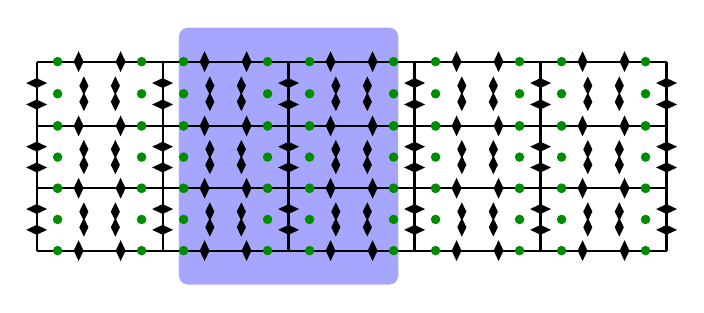
\begin{tikzpicture}[scale=8,
    on each segment/.style={
      decorate,
      decoration={
        show path construction,
        moveto code={},
        lineto code={
          \path [#1]
          (\tikzinputsegmentfirst) -- (\tikzinputsegmentlast);
        }}},
    nedof/.style={postaction={decorate, decoration={markings,
          mark=at position 1/3 with {
            \node[transform shape,shape=diamond,fill=black,draw=black,
            inner sep=0pt, minimum height=3pt, minimum width=6pt, rotate=90] {};
          },
          mark=at position 2/3 with {
            \node[transform shape,shape=diamond,fill=black,draw=black,
            inner sep=0pt, minimum height=3pt, minimum width=6pt, rotate=90] {};
          }}}},
    intdof/.style={shape=diamond, fill=black, draw=black, inner sep=0pt,
      minimum height=3pt, minimum width=6pt, rotate=90},
    bdof/.style={shape=circle, fill=green!55!black, draw=green!55!black,
      inner sep=0pt, minimum size=3pt}]

    % grid vertices: 5x3 quads -> 6x4 points
    \foreach \i/\k in {0/0,0.2/1,0.4/2,0.6/3,0.8/4,1.0/5} {
      \foreach \j/\l in {0/0,0.33/1,0.66/2,1.0/3} {
        \coordinate (v\k\l) at (\i, {0.3*\j});
      }
    }

    % ---- column patch shading (drawn first, behind markers) ----
    \coordinate (i10) at ($(v10) + (315:0.0564)$);
    \coordinate (i11) at ($(v11) - (180:0.04)$);
    \coordinate (i12) at ($(v12) - (180:0.04)$);
    \coordinate (i13) at ($(v13) + (45:0.0564)$);
    \coordinate (i30) at ($(v30) + (225:0.0564)$);
    \coordinate (i31) at ($(v31) - (0:0.04)$);
    \coordinate (i32) at ($(v32) - (0:0.04)$);
    \coordinate (i33) at ($(v33) + (135:0.0564)$);
    \path[fill=blue, opacity=0.35]
      \convexpath{i10,i11,i12,i13,i33,i32,i31,i30}{0.4pt};

    % ---- edges: two normal DOFs each (RT_2 edge moments) ----
    \foreach \l in {0,...,3}{
      \foreach \k in {0,...,4}{
        \pgfmathtruncatemacro{\ka}{\k+1}
        \draw[nedof, thick, black] (v\k\l) -- (v\ka\l);
      }
    }
    \foreach \k in {0,...,5}{
      \foreach \l in {0,...,2}{
        \pgfmathtruncatemacro{\lb}{\l+1}
        \draw[nedof, thick, black] (v\k\l) -- (v\k\lb);
      }
    }

    % ---- per-cell DOFs: velocity interior and buoyancy ----
    \foreach \k in {0,...,4}{
      \pgfmathtruncatemacro{\ka}{\k+1}
      \foreach \l in {0,...,2}{
        \pgfmathtruncatemacro{\lb}{\l+1}

        % velocity interior (RT_2): 2x2 cluster at (3/8, 5/8) x (3/8, 5/8)
        \coordinate (B1) at ($(v\k\l)!3/8!(v\ka\l)$);
        \coordinate (B2) at ($(v\k\l)!5/8!(v\ka\l)$);
        \coordinate (T1) at ($(v\k\lb)!3/8!(v\ka\lb)$);
        \coordinate (T2) at ($(v\k\lb)!5/8!(v\ka\lb)$);
        \node[intdof] at ($(B1)!3/8!(T1)$) {};
        \node[intdof] at ($(B2)!3/8!(T2)$) {};
        \node[intdof] at ($(B1)!5/8!(T1)$) {};
        \node[intdof] at ($(B2)!5/8!(T2)$) {};

        % buoyancy W^theta_2 = DG_1 x CG_2:
        % horizontal positions 1/6, 5/6; vertical positions 0, 1/2, 1
        \coordinate (B1) at ($(v\k\l)!1/6!(v\ka\l)$);
        \coordinate (B2) at ($(v\k\l)!5/6!(v\ka\l)$);
        \coordinate (T1) at ($(v\k\lb)!1/6!(v\ka\lb)$);
        \coordinate (T2) at ($(v\k\lb)!5/6!(v\ka\lb)$);
        \node[bdof] at (B1) {};
        \node[bdof] at (B2) {};
        \node[bdof] at ($(B1)!1/2!(T1)$) {};
        \node[bdof] at ($(B2)!1/2!(T2)$) {};
        \node[bdof] at (T1) {};
        \node[bdof] at (T2) {};
      }
    }

  \end{tikzpicture}
  \caption{Column star patch on a small aspect ratio quadrilateral mesh
    (\texttt{ExtrudedMesh}) for the velocity-buoyancy block obtained after
    Schur complement elimination of pressure. Black diamonds denote velocity
    DOFs ($\mathrm{RT}_2$) and green circles denote buoyancy DOFs
    ($\mathbb{W}_h^\theta = \mathrm{DG}_1 \otimes \mathrm{CG}_2$); the shaded region indicates the
    column patch subproblem on which the line smoother is applied.}
  \label{fig:patch-dofs}
\end{figure}
Figure~\ref{fig:patch-dofs} illustrates the
resulting degree-of-freedom layout on a representative small-aspect-ratio
extruded mesh, with the velocity and buoyancy degrees of freedom on one
star patch highlighted.

The column-patch smoother captures the strong vertical coupling
induced by the small aspect ratio $\varepsilon$: error modes that are
oscillatory along a column are resolved exactly within the patch,
while smooth, horizontally-varying modes are deferred to the coarse
grid correction. Standard point smoothers (Jacobi, Gauss--Seidel)
fail to damp the vertically-oscillatory modes and produce iteration
counts that grow as $\varepsilon \to 0$; the column patch restores
$\varepsilon$-robustness.

Explicitly, the local problem solved on patch $\omega_i$ is: find
$(u_i, b_i) \in X_i$ such that
\begin{align}
    s\bigl(R_i^\top(u_i, b_i),\, R_i^\top(w_i, q_i)\bigr)
    = \langle r,\, R_i^\top(w_i, q_i) \rangle
    \qquad \forall\, (w_i, q_i) \in X_i,
    \label{eq:patch-local}
\end{align}
where $r$ is the current residual of $S$ and $s(\cdot, \cdot)$ is the
bilinear form of~\eqref{eq:Schur-explicit}; this is precisely the
operator equation $A_i (u_i, b_i) = R_i r$ of the abstract
construction above, restricted to the velocity and buoyancy degrees of
freedom on the columns forming $\omega_i$. Because $X_i$ contains a
complete set of vertical-velocity and buoyancy degrees of freedom on
those columns together with the horizontal-velocity degrees of freedom
on their vertical facets, problem~\eqref{eq:patch-local} is itself a small, well-posed
velocity-buoyancy problem and is solved by a direct factorisation; this
is the solvability property invoked above and is what makes the patch
act as an exact line solve in the vertical direction. The patch
smoother is combined with the multigrid hierarchy in the usual
subspace-correction sense: relaxation
sweeps~\eqref{eq:patch-local} on the fine grid remove the
vertically-oscillatory error components patch by patch, and the coarse
grid correction, built by the standard geometric coarsening of the
extruded mesh in the horizontal direction, removes the remaining
smooth, horizontally-varying error. The implementation-level detail of
how this patch construction and Richardson relaxation are configured
in Firedrake~\cite{firedrake2016} and
PETSc~\cite{PETScUsersManual} for the experiments of
Section~\ref{sec:numerical} is given in
Appendix~\ref{app:petsc-options}.

\subsection{Algorithm summary}
\label{sec:algorithm}

The full preconditioner is summarised in
Figure~\ref{fig:preconditioner-flowchart}. At each time step, the
fully discrete system~\eqref{eq:fully-discrete} is solved by FGMRES
right-preconditioned by $A_\delta^{-1}$. The preconditioner is applied
via the Schur complement factorisation of Section~\ref{sec:schur},
with the pressure block inverted exactly by a block-diagonal direct
solve and the velocity-buoyancy block inverted approximately by a
multigrid V-cycle with column-patch smoothing.

\begin{figure}[t]
    \centering
    \resizebox{\linewidth}{!}{
    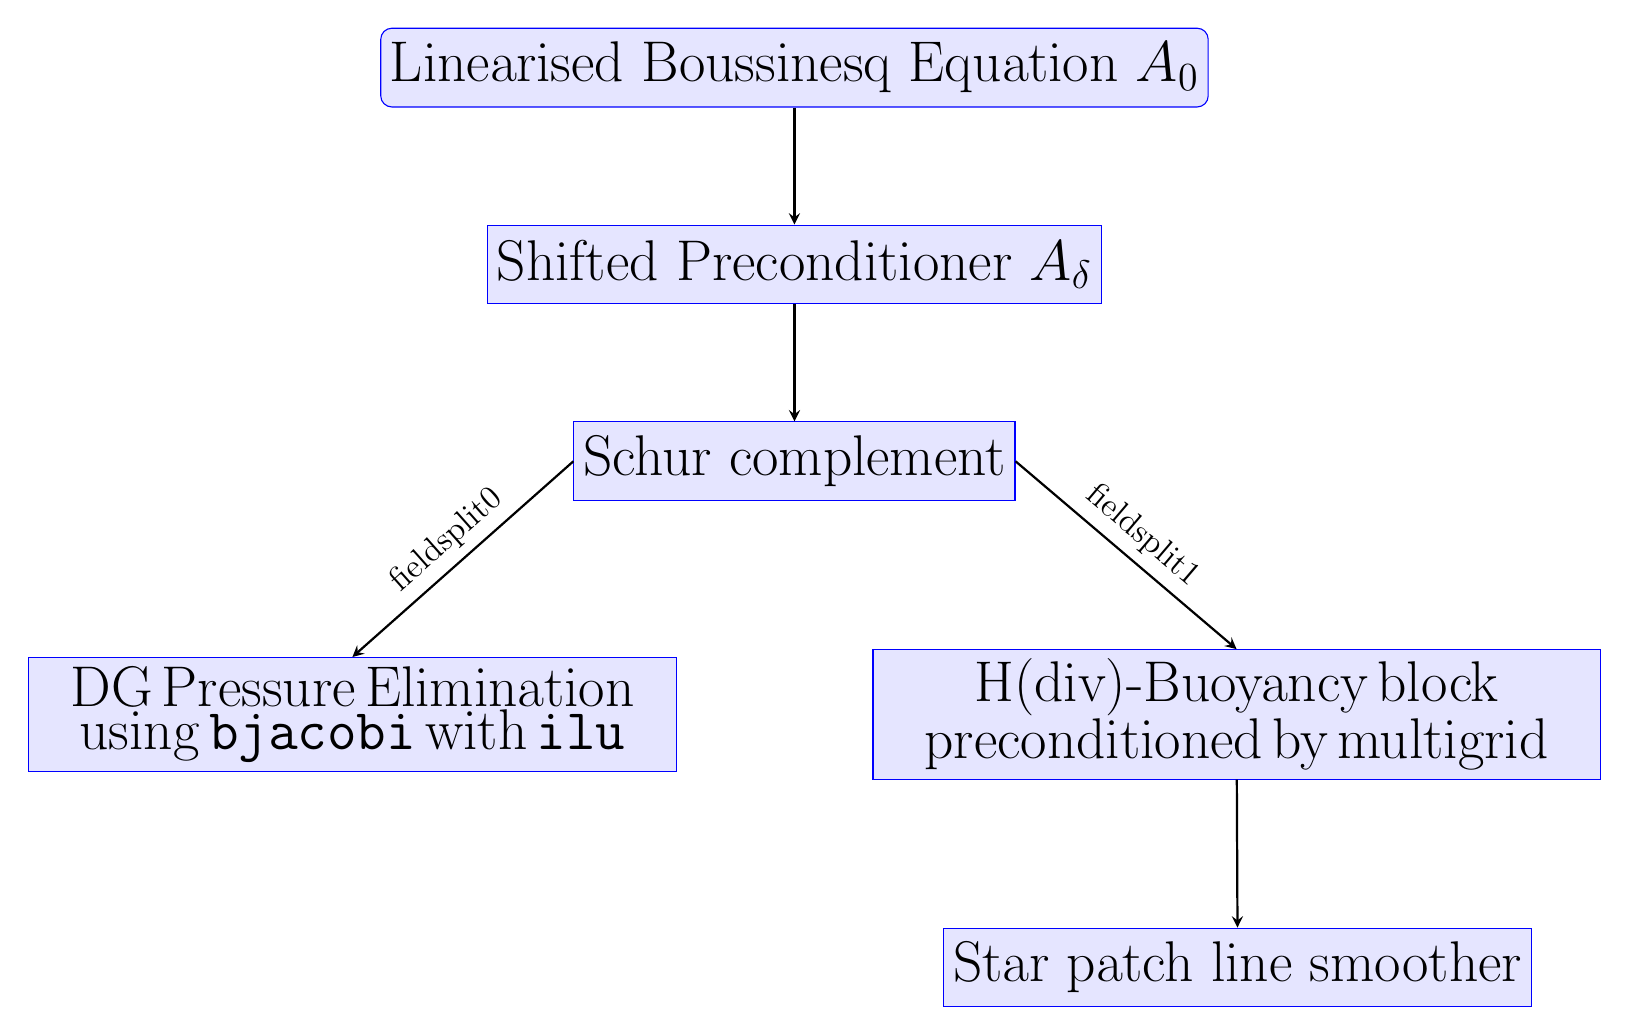
\begin{tikzpicture}[node distance=2cm]
    % Nodes
    \node (A) [startstop] {\huge Linearised Boussinesq Equation $A_0$};
    \node (B) [process, below of=A, yshift=-0.5cm] {\huge Shifted Preconditioner $A_{\delta}$};
    \node (C) [process, below of=B, yshift=-0.5cm] {\huge Schur complement};
    \node (D) [process, below left of=C, xshift=-4.2cm, yshift=-1.8cm, text width=8cm, align=center]
{\huge DG Pressure Elimination \\ using \texttt{bjacobi} with \texttt{ilu}};
    \node (E) [process, below right of=C, xshift=4.2cm, yshift=-1.8cm, text width=9cm, align=center] {\huge H(div)-Buoyancy block \\ preconditioned by multigrid};
    \node (F) [process, below right of=E, xshift=-1.4cm, yshift=-1.8cm] {\huge Star patch line smoother};

    % Arrows with labels
    \draw [arrow] (A) -- (B);
    \draw [arrow] (B) -- (C);
    \draw [arrow] (C.west) -- (D.north) node[midway, above, sloped, font=\large] {fieldsplit0};
    \draw [arrow] (C.east) -- (E.north) node[midway, above, sloped, font=\large] {fieldsplit1};
    \draw [arrow] (E) -- (F);
    % \draw [arrow] (E) -- (F) node[midway, above, sloped, font=\large] {smoother};
    \end{tikzpicture}
    }
    \caption{Algorithmic structure of the shifted-Schur preconditioner: the
    fully discrete system $A_0$ is preconditioned by the shifted matrix
    $A_\delta$, whose Schur complement splits via \texttt{fieldsplit} into
    an exact pressure mass solve (left branch) and a multigrid V-cycle on
    the velocity-buoyancy block $S$ with column-patch (star) line
    smoothing (right branch).}
    \label{fig:preconditioner-flowchart}
\end{figure}



\section{Theoretical analysis of the shifted preconditioner}
\label{sec:theory}

In this section, we establish the rigorous bound on the spectral 
distance between the shifted operator $\mathcal{A}_\delta$ and the original 
operator $\mathcal{A}_0$ that motivates the preconditioning strategy of 
Section~\ref{sec:precond}. The analysis proceeds in three steps. 
First, we reduce the bound to a well-posedness question for a 
perturbed mixed variational problem by eliminating the buoyancy
variable explicitly. Second, we verify the Brezzi-type conditions on
the resulting perturbed problem, obtaining quantitative estimates for
the kernel coercivity constant, the inf--sup constant, and the
operator norm of the bilinear form.  Because the Coriolis term makes
the velocity block nonsymmetric, the bound is then drawn from the
nonsymmetric perturbed saddle-point theory
of~\cite{ciarletHuangZou2003} rather than from the symmetric perturbed
Brezzi theory of~\cite{boffi2013mixed}; the hypotheses that this
requires are coercivity on the constraint kernel alone, which is what
the problem supplies.  Third, we combine these to state the main bound
and derive the asymptotic scaling of the shift parameter $\delta$ in
terms of the time step $\Delta t$, the buoyancy frequency $N$, and the
aspect ratio of the domain.

The analysis is performed at the continuous level. The corresponding 
discrete statement carries through verbatim provided the compatible 
finite element triple~\eqref{eq:fe-triple} is used, since this triple 
inherits the inf--sup condition from the continuous setting; we make 
this explicit at the end of Section~\ref{sec:main-bound}.

% 
\subsection{Reduction to a perturbed mixed problem}
\label{sec:reduction}

We work with the fully discrete linearised Boussinesq 
system~\eqref{eq:fully-discrete} at a single time step, with the 
known stage-$n$ data collected into the right-hand sides. For 
brevity we relabel the unknowns $\vec{u}'^{\,n+1}, b'^{\,n+1}, 
p'^{\,n+1}$ as $u, b, p$ throughout this section. The 
system~\eqref{eq:fully-discrete} can be written as
\begin{subequations}\label{eq:fully-discrete-relabelled}
\begin{align}
    \langle w, u \rangle 
    + \Delta t \langle w, \Omega \times u \rangle
    - \Delta t \langle \nabla \cdot w, p \rangle
    - \tfrac{\Delta t}{2} \langle w, b \hat{k} \rangle
    &= \langle f, w \rangle, \\
    \langle q, b \rangle + \tfrac{\Delta t N^2}{2} \langle u \cdot \hat{k}, q \rangle
    &= \langle g, q \rangle, \\
    \langle \nabla \cdot u, \phi \rangle &= 0,
\end{align}
\end{subequations}
for all test functions $(w, q, \phi) \in V \times B \times Q$, 
where $V = H(\mathrm{div}; \Omega)$ with no-flux essential boundary 
condition, $B = L^2(\Omega)$, $Q = L^2_0(\Omega)$, and the right-hand 
sides $f, g$ encode the stage-$n$ data.

We define the bilinear forms $\mathcal{A}_0, \mathcal{A}_\delta$ on the
product space $V \times B \times Q$ by
\begin{align}
    \mathcal{A}_0[u, b, p;\, w, q, \phi] 
    &:= \langle w, u \rangle 
    + \Delta t \langle w, \Omega \times u \rangle 
    - \Delta t \langle \nabla \cdot w, p \rangle 
    \nonumber\\
    &\quad{} - \tfrac{\Delta t}{2} \langle w, b \hat{k} \rangle
    + \langle q, b \rangle 
    + \tfrac{\Delta t N^2}{2} \langle u \cdot \hat{k}, q \rangle
    + \langle \nabla \cdot u, \phi \rangle,
    \label{eq:A0-def}\\
    \mathcal{A}_\delta[u, b, p;\, w, q, \phi] 
    &:= \mathcal{A}_0[u, b, p;\, w, q, \phi] 
    + \delta \langle p, \phi \rangle.
    \label{eq:Adelta-def}
\end{align}
Each of the two forms induces, in the usual way, a linear operator
from $V \times B \times Q$ to its dual, and we use the same symbols
$\mathcal{A}_0$, $\mathcal{A}_\delta$ for these operators; it is in
this sense that compositions such as
$\mathcal{A}_\delta^{-1} \mathcal{A}_0$ are understood below. The
matrices $A_0$ and $A_\delta$ of Section~\ref{sec:precond} are the
finite element representations of the corresponding discrete
variational problems; matrix notation was used there only to display
the block structure of the solver, and plays no further role in the
analysis, which is carried out at the continuous variational level,
the discrete statement being recovered at the end of
Section~\ref{sec:main-bound}.

To bound the spectral distance $\|\mathcal{A}_\delta^{-1} \mathcal{A}_0 - I\|$, we set
$[u_1, b_1, p_1] := (\mathcal{A}_\delta^{-1} \mathcal{A}_0 - I)[u_0, b_0, p_0]$ for
arbitrary input $[u_0, b_0, p_0] \in V \times B \times Q$. Applying
$\mathcal{A}_\delta$ to both sides and using $\mathcal{A}_0 - \mathcal{A}_\delta = -\delta
\langle p, \phi \rangle$ yields the perturbed problem
\begin{subequations}\label{eq:perturbed-3x3}
\begin{align}
    \langle w, u_1 \rangle 
    + \Delta t \langle w, \Omega \times u_1 \rangle
    - \Delta t \langle \nabla \cdot w, p_1 \rangle
    - \tfrac{\Delta t}{2} \langle w, b_1 \hat{k} \rangle
    &= 0,
    \label{eq:perturbed-mom}\\
    \langle q, b_1 \rangle + \tfrac{\Delta t N^2}{2} \langle u_1 \cdot \hat{k}, q \rangle
    &= 0,
    \label{eq:perturbed-buoy}\\
    \langle \nabla \cdot u_1, \phi \rangle + \delta \langle p_1, \phi \rangle
    &= -\delta \langle p_0, \phi \rangle,
    \label{eq:perturbed-div}
\end{align}
\end{subequations}
for all $(w, q, \phi) \in V \times B \times Q$. The bound on 
$\|\mathcal{A}_\delta^{-1} \mathcal{A}_0 - I\|$ is thus reduced to a well-posedness 
question for~\eqref{eq:perturbed-3x3}: a bound on $\|(u_1, p_1)\|$ in 
terms of $\delta \|p_0\|$ translates directly into a bound on the 
operator norm via supremum over $(u_0, b_0, p_0)$.

We eliminate $b_1$ from~\eqref{eq:perturbed-buoy} by setting 
$q = b_1$, which gives 
$\langle b_1, q \rangle = -\tfrac{\Delta t N^2}{2} \langle u_1 \cdot \hat{k}, q \rangle$ 
for all $q \in B$. Substituting into~\eqref{eq:perturbed-mom} via 
$\tfrac{\Delta t}{2} \langle w, b_1 \hat{k} \rangle 
= \tfrac{\Delta t}{2} \langle w \cdot \hat{k}, b_1 \rangle 
= -\tfrac{\Delta t^2 N^2}{4} \langle w \cdot \hat{k}, u_1 \cdot \hat{k} \rangle$
gives, after dropping the subscript on $u, p$ for readability,
\begin{subequations}\label{eq:perturbed-2x2}
\begin{align}
    \left\langle \tfrac{M}{\Delta t} u, w \right\rangle 
    + \langle \Omega \times u, w \rangle
    - \langle \nabla \cdot w, p \rangle
    &= 0,
    \label{eq:perturbed-2x2-mom}\\
    - \langle \nabla \cdot u, \phi \rangle - \delta \langle p, \phi \rangle
    &= \delta \langle p_0, \phi \rangle,
    \label{eq:perturbed-2x2-div}
\end{align}
\end{subequations}
where we have rescaled by $\Delta t$ for symmetry and where
\begin{align}
    M := I + \frac{\Delta t^2 N^2}{4}\, \hat{k} \otimes \hat{k}.
    \label{eq:M-def}
\end{align}
The operator $M$ is symmetric positive definite, with eigenvalues $1$ 
(on the horizontal components) and $1 + \tfrac{\Delta t^2 N^2}{4}$ 
(on the vertical component).

The system~\eqref{eq:perturbed-2x2} is of the form
\begin{align}
    a(u, w) + b(w, p) &= F[w], \\
    b(u, \phi) - c(p, \phi) &= G[\phi],
\end{align}
with
\begin{align}
    a(u, w) &= \left\langle \tfrac{M}{\Delta t} u, w \right\rangle 
    + \langle \Omega \times u, w \rangle,
    \label{eq:a-def}\\
    b(w, p) &= -\langle \nabla \cdot w, p \rangle,
    \label{eq:b-def}\\
    c(p, \phi) &= \delta \langle p, \phi \rangle,
    \label{eq:c-def}\\
    F[w] &= 0, \qquad G[\phi] = \delta \langle p_0, \phi \rangle,
\end{align}
the sign of $G$ following from~\eqref{eq:perturbed-div} on
multiplication by $-1$.  Only $\|G\| \le \delta\|p_0\|$ enters the
estimates below, so the sign is immaterial to the bound.
This is a perturbed saddle point problem of the kind treated
in~\cite{boffi2013mixed} for symmetric $a$ and
in~\cite{ciarletHuangZou2003} without a symmetry assumption; both
provide quantitative well-posedness of mixed problems carrying a
lower-right perturbation $c(\cdot,\cdot)$.  The Coriolis term makes
$a$ nonsymmetric here, so it is the latter that we use; see
Section~\ref{sec:main-bound}.

\begin{rem}
\label{rem:b1-elimination}
The elimination of $b_1$ is exact at the continuous level, holding in 
the $L^2$ sense. At the discrete level it holds whenever the 
compatible finite element triple~\eqref{eq:fe-triple} is used and the
boundary and the mesh layers are flat, since the vertical-component test space and the 
buoyancy space agree on horizontal facets. This is the structural 
reason why the discrete inf--sup constant inherits the continuous 
estimate, and is the key advantage of the tensor-product buoyancy 
space $\mathbb{W}_h^\theta$ of~\cite{natale2016compatible, melvin2018choice} over a fully discontinuous alternative.
\end{rem}

\subsection{Brezzi conditions}
\label{sec:brezzi}

We verify the hypotheses required by the abstract perturbed
saddle-point theory of Section~\ref{sec:main-bound} on
problem~\eqref{eq:perturbed-2x2}.  Two choices are made before the
estimates begin, and both are made in order to expose the aspect-ratio
and time-step dependence of the constants rather than to bury it
inside them: the domain is rescaled in the vertical, and the velocity
space is given a norm weighted by the stratification operator $M$.

Throughout, the analysis is carried out in rescaled variables,
with horizontal lengths measured in units of the horizontal extent of
$\Omega$, times in units of a reference time, and the vertical
coordinate rescaled by $\hat{z} = z / \varepsilon$, where
$\varepsilon$ is the aspect ratio.  Here $z$ is already the
non-dimensional vertical coordinate, measured, like the horizontal
lengths, in units of $L_x$, so that $z$ ranges over $(0,\varepsilon)$
and $\hat{z}$ over $(0,1)$; equivalently, $\hat{z}$ is the
depth-normalised coordinate $z_{\mathrm{phys}}/L_z$.  The rescaled
domain $\hat\Omega$
then has unit extent in every coordinate direction and is
independent of $\varepsilon$. All of the anisotropy is carried
instead by the divergence operator, which becomes
\begin{align}
    \nabla_{\varepsilon} \cdot \vec{v}
    := \pder{v_1}{x} + \pder{v_2}{y}
       + \frac{1}{\varepsilon}\pder{v_3}{\hat{z}} .
    \label{eq:div-eps}
\end{align}
This is the same operator as $\nabla\cdot$ written in the original
coordinates, so no equation changes. What changes is that the
auxiliary problems used to estimate the inf--sup constant in
Lemma~\ref{lem:inf-sup} are now posed on a fixed domain rather than on
one that degenerates as $\varepsilon\to0$, and the $\varepsilon$
dependence of the constants can be read off directly.  We write
$\Delta_\varepsilon := \nabla_\varepsilon\cdot\nabla_\varepsilon$ for
the correspondingly rescaled Laplacian.

For the spaces, we take
\begin{align}
    V = \mathring{H}(\mathrm{div}_\varepsilon;\, \hat\Omega),
    \qquad
    Q = L^2_0(\hat\Omega),
\end{align}
where the circle denotes the no-flux essential condition
$\vec{v}\cdot\hat{n} = 0$ and $L^2_0$ is the space of square-integrable
functions of zero mean.  Restricting $Q$ to $L^2_0$ removes the 
constant pressure mode, which is the physical nullspace of the
unshifted operator $\mathcal{A}_0$ and on which no bound is asserted.  The
velocity space carries the \emph{$M$-weighted graph norm}
\begin{align}
    \|\vec{v}\|_V^2
    := \frac{1}{\Delta t}\left\langle M \vec{v},\, \vec{v}\right\rangle
       + \|\nabla_\varepsilon \cdot \vec{v}\|_{L^2}^2 ,
    \label{eq:V-norm}
\end{align}
with $M$ as in~\eqref{eq:M-def}, and $Q$ carries the $L^2$ norm.
Weighting by $M/\Delta t$ rather than using the plain graph norm
$\|\vec{v}\|_{L^2}^2 + \|\nabla_\varepsilon\cdot\vec{v}\|_{L^2}^2$
absorbs the stratification into the metric.  Fitting the norm to the
operator in this way, so that the parameter dependence is carried by
the metric rather than by the constants, is the strategy of
Zulehner~\cite{zulehner2011} for obtaining parameter-robust estimates
for saddle point problems, and it is what makes the constants of
Lemmas~\ref{lem:coercivity} and~\ref{lem:a-norm} independent of
$\Delta t$ and $N$.

It is convenient to abbreviate
\begin{align}
    m := \lambda_{\max}(M) = 1 + \frac{\Delta t^2 N^2}{4},
    \qquad
    J\vec{v} := \Omega \times \vec{v},
    \label{eq:m-J-def}
\end{align}
so that the form~\eqref{eq:a-def} reads
$a(\vec{u},\vec{w}) = \tfrac{1}{\Delta t}\langle M\vec{u},\vec{w}\rangle
+ \langle J\vec{u},\vec{w}\rangle$.  On the $f$-plane
$\Omega = (0,0,f/2)$, so that $2\Omega\times\vec{u} = f\,\hat{k}\times\vec{u}$
recovers the Coriolis term of Section~\ref{sec:governing} with $f$ the
Coriolis parameter, and $\|J\|_2 = f/2$.

The kernel associated with the bilinear form $b$ is
\begin{align}
    K := \left\{\vec{v}\in V \;:\; b(\vec{v}, q) = 0
    \ \text{ for all } q \in Q\right\}.
    \label{eq:kernel-def}
\end{align}
Since $Q = L^2_0$ excludes constants, membership of $K$ says only that
$\nabla_\varepsilon\cdot\vec{v}$ is zero.  Hence
\begin{align}
    K = \left\{\vec{v}\in V \;:\;
    \nabla_\varepsilon\cdot\vec{v} = 0\right\},
    \label{eq:kernel-divfree}
\end{align}
which is precisely the subspace on which the norm~\eqref{eq:V-norm}
collapses to its first term. Coercivity will be required on $K$
alone and not on all of $V$.

\begin{lem}[Kernel coercivity and the constraint norms]
\label{lem:coercivity}
With respect to the norm~\eqref{eq:V-norm}, the bilinear form $a$
of~\eqref{eq:a-def} satisfies
\begin{align}
    a(\vec{v}, \vec{v}) = \|\vec{v}\|_V^2
    \qquad \forall\, \vec{v} \in K ,
    \label{eq:coercivity-alpha}
\end{align}
so that the coercivity constant is $\alpha = 1$, exactly, with no
dependence on $\Delta t$, $N$, $f$ or the aspect ratio $\varepsilon$.
Moreover $\|b\| = 1$ and $\|c\| = \delta$.
\end{lem}

\begin{proof}
For $\vec{v}\in K$ we have $\nabla_\varepsilon\cdot\vec{v} = 0$
by~\eqref{eq:kernel-divfree}, so that
$\|\vec{v}\|_V^2 = \tfrac{1}{\Delta t}\langle M\vec{v},\vec{v}\rangle$.
The Coriolis operator is skew, $\langle J\vec{v},\vec{v}\rangle = 0$
pointwise by antisymmetry of the cross product, so it contributes
nothing to the quadratic form and
\begin{align}
    a(\vec{v},\vec{v})
    = \tfrac{1}{\Delta t}\langle M\vec{v},\vec{v}\rangle
      + \langle J\vec{v},\vec{v}\rangle
    = \tfrac{1}{\Delta t}\langle M\vec{v},\vec{v}\rangle
    = \|\vec{v}\|_V^2 .
\end{align}
This is an equality, not a lower bound, so $\alpha = 1$ is
attained.  For $b$, the graph norm structure of~\eqref{eq:V-norm} gives
$\|\nabla_\varepsilon\cdot\vec{v}\|_{L^2}\le\|\vec{v}\|_V$ and hence
$|b(\vec{v},q)| \le \|\vec{v}\|_V\|q\|_Q$, so $\|b\|\le1$.  
Finally
$\|c\| = \delta$ is immediate from
$c(p,\phi) = \delta\langle p,\phi\rangle$.
\end{proof}

% \begin{rem}
% \label{rem:weighted-norm}
% The identity~\eqref{eq:coercivity-alpha} is the reason for
% adopting~\eqref{eq:V-norm}.  Under the plain graph norm \cjc{you didn't define that.
% Probably this discussion isn't needed, just useful for your notes.} \mh{Yes.}
% the same
% computation gives only $\alpha = 1/\Delta t$, while the operator norm
% of $a$ grows like $m/\Delta t$, so that the ratio $\|a\|/\alpha$ --- the
% quantity that actually enters the smallness
% condition~\eqref{eq:delta2-def} --- becomes the condition number $m$ of
% $M$ rather than a constant of order one.  Remark~\ref{rem:graph-norm}
% quantifies the resulting loss.
% \end{rem}

The inf--sup condition on $b$ is the key result of this section.
Since $b(\vec{v},q)$ depends on $\vec{v}$ only through
$\nabla_\varepsilon\cdot\vec{v}$, bounding its supremum from below
amounts to exhibiting, for each $q$, a velocity field whose divergence
is $-q$ and whose $V$-norm is as small as possible.  We therefore
construct that field first, and establish that the constants it defines
are finite; the inf--sup estimate is then immediate.

\begin{lem}[Right inverse of the rescaled divergence]
\label{lem:right-inverse}
Let $\hat\Omega$ be connected with Lipschitz boundary.  For every
$q\in Q = L^2_0(\hat\Omega)$ the auxiliary Neumann problem
\begin{align}
    -\Delta_\varepsilon \phi = q \ \text{ in } \hat\Omega,
    \qquad
    \nabla_\varepsilon\phi\cdot\hat{n} = 0
    \ \text{ on } \partial\hat\Omega,
    \qquad
    \int_{\hat\Omega}\phi = 0,
    \label{eq:aux-neumann}
\end{align}
has a unique solution, and $\mathcal{R}q := \nabla_\varepsilon\phi$
defines a linear map $\mathcal{R}: Q\to V$ with the following
properties.
\begin{enumerate}
    \item[(i)] \emph{Right inverse.} $\mathcal{R}q\in V$ and
    $\nabla_\varepsilon\cdot\mathcal{R}q = -q$.
    \item[(ii)] \emph{Minimality.} $\|\mathcal{R}q\|_{L^2}
    \le \|\vec{v}\|_{L^2}$ for every $\vec{v}\in V$ with
    $\nabla_\varepsilon\cdot\vec{v} = -q$.
    \item[(iii)] \emph{Finiteness.} The two right-inverse constants
    \begin{align}
        C_P := \sup_{q\in Q,\, q\neq0}
        \frac{\|\mathcal{R}q\|_{L^2}}{\|q\|_{L^2}},
        \qquad
        C_M := \sup_{q\in Q,\, q\neq0}
        \frac{\left\langle M\mathcal{R}q,\,
              \mathcal{R}q\right\rangle^{1/2}}{\|q\|_{L^2}}
        \label{eq:CP-def}
    \end{align}
    are finite, and
    \begin{align}
        C_P = \nu_{\min}^{-1/2},
        \qquad
        C_M \le \sqrt{m}\,C_P ,
        \label{eq:CP-spectral}
    \end{align}
    where $\nu_{\min}>0$ is the smallest nonzero eigenvalue of
    $-\Delta_\varepsilon$ on $\hat\Omega$ under the boundary conditions
    of~\eqref{eq:aux-neumann}.
\end{enumerate}
Here $C_P$ measures, in $L^2$, how large a velocity field must be in
order to realise a prescribed divergence; it is a property of the
geometry alone.  The constant $C_M$ measures the same field in the
stratification-weighted metric $\langle M\cdot,\cdot\rangle$, and it is
$C_M$ that enters the estimates below, because $\|\cdot\|_V$ weights
the velocity by $M/\Delta t$.
\end{lem}

\begin{proof}
\emph{Existence and uniqueness.}  The weak form
of~\eqref{eq:aux-neumann} is: find $\phi\in H^1(\hat\Omega)\cap L^2_0$
with $\langle\nabla_\varepsilon\phi,\nabla_\varepsilon\psi\rangle
= \langle q,\psi\rangle$ for all $\psi\in H^1(\hat\Omega)\cap L^2_0$.
The form is bounded, and coercive on $H^1\cap L^2_0$ by the
Poincar\'e--Wirtinger inequality
\begin{align}
    \|\psi\|_{L^2}
    \;\le\; \nu_{\min}^{-1/2}\,\|\nabla_\varepsilon\psi\|_{L^2}
    \qquad \forall\,\psi\in H^1(\hat\Omega)\cap L^2_0 ,
    \label{eq:poincare-wirtinger}
\end{align}
which holds with $\nu_{\min}>0$ because $\hat\Omega$ is connected and
the embedding $H^1(\hat\Omega)\hookrightarrow L^2(\hat\Omega)$ is
compact.  The constraint $q\in L^2_0$ is exactly the compatibility
condition for the Neumann problem, so Lax--Milgram gives a unique
$\phi$.

\emph{(i).}  By construction
$\mathcal{R}q = \nabla_\varepsilon\phi\in L^2(\hat\Omega)$ and
$\nabla_\varepsilon\cdot\mathcal{R}q = \Delta_\varepsilon\phi = -q
\in L^2(\hat\Omega)$, so
$\mathcal{R}q\in H(\mathrm{div}_\varepsilon;\hat\Omega)$.  Its normal
trace is $\mathcal{R}q\cdot\hat{n} =
\nabla_\varepsilon\phi\cdot\hat{n} = 0$, which is the no-flux
condition, so $\mathcal{R}q\in\mathring{H}(\mathrm{div}_\varepsilon) = V$.

\emph{(ii).}  Let $\vec{v}\in V$ with
$\nabla_\varepsilon\cdot\vec{v} = -q$, and put
$\vec{v}_0 := \vec{v} - \mathcal{R}q$, so that
$\nabla_\varepsilon\cdot\vec{v}_0 = 0$ and $\vec{v}_0\cdot\hat{n} = 0$.
Integrating by parts,
\begin{align}
    \left\langle \mathcal{R}q,\, \vec{v}_0\right\rangle
    = \left\langle \nabla_\varepsilon\phi,\, \vec{v}_0\right\rangle
    = -\left\langle \phi,\,
      \nabla_\varepsilon\cdot\vec{v}_0\right\rangle
      + \int_{\partial\hat\Omega}\phi\,\vec{v}_0\cdot\hat{n}
    = 0 ,
    \label{eq:helmholtz-orthogonality}
\end{align}
both terms vanishing, the first because $\vec{v}_0$ is
divergence-free and the second because $\vec{v}_0\in V$.  Hence
$\|\vec{v}\|_{L^2}^2 = \|\mathcal{R}q\|_{L^2}^2
+ \|\vec{v}_0\|_{L^2}^2 \ge \|\mathcal{R}q\|_{L^2}^2$.

\emph{(iii).}  Let $\{\psi_k\}$ be an $L^2$-orthonormal basis of
eigenfunctions of $-\Delta_\varepsilon$ under the boundary conditions
of~\eqref{eq:aux-neumann}, with eigenvalues $\nu_k$; the zero-mean
constraint excludes the eigenvalue $0$, so $\nu_k\ge\nu_{\min}>0$.
Integration by parts gives
$\langle\nabla_\varepsilon\psi_j,\nabla_\varepsilon\psi_k\rangle
= \nu_k\delta_{jk}$.  For $q = \sum_k c_k\psi_k$ we have
$\phi = \sum_k \nu_k^{-1}c_k\psi_k$, hence
\begin{align}
    \frac{\|\mathcal{R}q\|_{L^2}^2}{\|q\|_{L^2}^2}
    = \frac{\sum_k \nu_k^{-2}c_k^2\,\nu_k}{\sum_k c_k^2}
    = \frac{\sum_k c_k^2/\nu_k}{\sum_k c_k^2}
    \;\le\; \frac{1}{\nu_{\min}} ,
\end{align}
with equality when $q$ is an eigenfunction for $\nu_{\min}$.  This
gives $C_P = \nu_{\min}^{-1/2}$, finite
by~\eqref{eq:poincare-wirtinger}.  Finally
$\langle M\vec{w},\vec{w}\rangle\le m\|\vec{w}\|_{L^2}^2$
by~\eqref{eq:m-J-def}, so $C_M\le\sqrt{m}\,C_P<\infty$.
\end{proof}

\begin{lem}[Inf--sup constant of $b(\cdot,\cdot)$]
\label{lem:inf-sup}
With $\mathcal{R}$, $C_M$ and $C_P$ as in
Lemma~\ref{lem:right-inverse}, the inf--sup condition holds:
\begin{align}
    \inf_{q\in Q}\, \sup_{\vec{v}\in V}
    \frac{b(\vec{v}, q)}{\|q\|_Q \|\vec{v}\|_V}
    \;\ge\; \beta
    := \left(1 + \frac{C_M^2}{\Delta t}\right)^{-1/2}
    \;\ge\; \left(1 + \frac{m\, C_P^2}{\Delta t}\right)^{-1/2}
    \;>\; 0 .
    \label{eq:beta-explicit}
\end{align}
\end{lem}

\begin{proof}
Fix $q\in Q$ and take $\vec{v} := \mathcal{R}q$, which lies in $V$ by
Lemma~\ref{lem:right-inverse}(i).  Then
\begin{align}
    b(\vec{v}, q)
    = -\left\langle \nabla_\varepsilon\cdot\vec{v},\, q\right\rangle
    = \|q\|_{L^2}^2 .
\end{align}
Using $\nabla_\varepsilon\cdot\vec{v} = -q$ in the second term
of~\eqref{eq:V-norm} and the definition~\eqref{eq:CP-def} of $C_M$ in
the first,
\begin{align}
    \|\vec{v}\|_V^2
    = \frac{1}{\Delta t}
      \left\langle M\mathcal{R}q,\, \mathcal{R}q\right\rangle
      + \|q\|_{L^2}^2
    \le \left(1 + \frac{C_M^2}{\Delta t}\right)\|q\|_{L^2}^2 ,
\end{align}
so that $b(\vec{v},q)/\|\vec{v}\|_V \ge \beta\|q\|_Q$.  Taking the
supremum over $\vec{v}\in V$ and then the infimum over $q\in Q$ gives
the first inequality; the second follows from
$C_M\le\sqrt{m}\,C_P$.  Both are strictly positive because $C_M$ is
finite, by Lemma~\ref{lem:right-inverse}(iii).
\end{proof}


We now make the $\varepsilon$-dependence of these constants explicit.
The inf--sup constant of Lemma~\ref{lem:inf-sup} depends on the
geometry only through $C_M$, and on a product domain the Poincar\'e
constants split into a horizontal and a vertical contribution, with
all of the $\varepsilon$-dependence carried by the vertical one.

\begin{lem}[Horizontal--vertical splitting of the Poincar\'e constant]
\label{lem:poincare-split}
Suppose the rescaled domain is a product,
$\hat\Omega = \omega \times (0,1)$, with $\omega$ a connected
Lipschitz horizontal domain carrying periodic or homogeneous Neumann
(free-slip) lateral conditions, and with the Neumann conditions
of~\eqref{eq:aux-neumann} at $\hat{z} \in \{0,1\}$.  Let $A_1 > 0$ be
the smallest nonzero eigenvalue of the horizontal Laplacian
$-\Delta_h$ on $\omega$, and let $\lambda_1 > 0$ be the smallest
nonzero eigenvalue of the vertical operator
$-\partial^2/\partial\hat{z}^2$ on the unit interval $(0,1)$ under
the top and bottom conditions of~\eqref{eq:aux-neumann}.  Define the
horizontal and vertical Poincar\'e constants
\begin{align}
    C_h := A_1^{-1/2},
    \qquad
    C_v := \varepsilon\,\hat{C}_v,
    \qquad
    \hat{C}_v := \lambda_1^{-1/2},
    \label{eq:Ch-Cv-def}
\end{align}
so that $C_v$ is the Poincar\'e constant of the rescaled vertical
operator $-\varepsilon^{-2}\,\partial^2/\partial\hat{z}^2$ on
$(0,1)$.  Since $\omega$ is the rescaled horizontal domain and
$\hat{C}_v$ is a constant of the unit interval, both $C_h$ and
$\hat{C}_v$ are independent of $\varepsilon$, and all of the
$\varepsilon$-dependence is carried by $C_v$.  For the rigid-lid
(Neumann) conditions used throughout this report, $\lambda_1 = \pi^2$,
so $\hat{C}_v = 1/\pi$ and $C_v = \varepsilon/\pi$.  Then
\begin{align}
    C_P = \max(C_h,\, C_v),
    \qquad
    C_M^2 = \max\!\left(C_h^2,\; m\,C_v^2\right).
    \label{eq:CP-CM-split}
\end{align}
In particular, whenever $\sqrt{m}\,C_v \le C_h$, we have
$C_M = C_P = C_h$, with no dependence on $\varepsilon$, $\Delta t$
or $N$.
\end{lem}

\begin{proof}
On the product domain the eigenfunctions of $-\Delta_\varepsilon$
under the stated boundary conditions separate: they are products
$\psi_{jl} = \phi_j\, v_l$ of eigenfunctions $\phi_j$ of $-\Delta_h$
on $\omega$ (eigenvalues $A_j$ listed in increasing order with
multiplicity, $A_0 = 0$ for the constant mode, so that $A_1$ is the
smallest nonzero eigenvalue of the statement) and eigenfunctions
$v_l$ of the vertical operator on $(0,1)$
(eigenvalues $B_l = \lambda_l/\varepsilon^2$ with
$\lambda_0 = 0 < \lambda_1 \le \cdots$, the factor $1/\varepsilon^2$
arising from the vertical part of~\eqref{eq:div-eps}; for the
rigid-lid conditions these are the Neumann modes
$v_l(\hat{z}) = \cos(\pi l \hat{z})$ with $\lambda_l = \pi^2 l^2$), so
that
$\nu_{jl} = A_j + B_l$ are the eigenvalues. The zero-mean constraint excludes
$(j,l) = (0,0)$.  Normalise $\|\psi_{jl}\|_{L^2} = 1$ and take
$q = \psi_{jl}$.  The auxiliary solution of~\eqref{eq:aux-neumann} is
then $\phi = \nu_{jl}^{-1}\psi_{jl}$, so
$\mathcal{R}q = \nu_{jl}^{-1}\nabla_\varepsilon\psi_{jl}$, whose
horizontal part is $\nu_{jl}^{-1}(\nabla_h\phi_j)\,v_l$ and whose
vertical part is
$\nu_{jl}^{-1}\varepsilon^{-1}\phi_j\,v_l'\,\hat{k}$.  Integrating by
parts under the stated boundary conditions,
\begin{align}
    \|\nabla_h\psi_{jl}\|_{L^2}^2
    = \left\langle -\Delta_h\psi_{jl},\, \psi_{jl}\right\rangle
    = A_j,
    \qquad
    \|\varepsilon^{-1}\partial_{\hat{z}}\psi_{jl}\|_{L^2}^2
    = \left\langle -\varepsilon^{-2}\partial_{\hat{z}\hat{z}}
      \psi_{jl},\, \psi_{jl}\right\rangle
    = B_l,
\end{align}
so the horizontal and vertical parts of $\nabla_\varepsilon\psi_{jl}$
carry $A_j$ and $B_l$ respectively, and
\begin{align}
    \|\mathcal{R}q\|_{L^2}^2
    = \nu_{jl}^{-2}\left(A_j + B_l\right)
    = \frac{1}{\nu_{jl}} .
\end{align}
Since $M = I + \tfrac{\Delta t^2 N^2}{4}\,\hat{k}\otimes\hat{k}$ acts
as the identity on the horizontal components and multiplies the
vertical component by $m$,
\begin{align}
    \left\langle M\mathcal{R}q,\, \mathcal{R}q\right\rangle
    = \frac{1}{\nu_{jl}^2}
      \left\langle M\nabla_\varepsilon\psi_{jl},\,
      \nabla_\varepsilon\psi_{jl}\right\rangle
    = \frac{1}{\nu_{jl}^2}
      \left(\|\nabla_h\psi_{jl}\|_{L^2}^2
      + m\,\|\varepsilon^{-1}\partial_{\hat{z}}\psi_{jl}\|_{L^2}^2\right)
    = \frac{A_j + m B_l}{\nu_{jl}^2}.
\end{align}
Hence
\begin{align}
    \frac{\|\mathcal{R}q\|_{L^2}^2}{\|q\|_{L^2}^2}
    = \frac{1}{\nu_{jl}} ,
    \qquad
    \frac{\left\langle M\mathcal{R}q,\, \mathcal{R}q\right\rangle}
         {\|q\|_{L^2}^2}
    = g(A_j, B_l),
    \qquad
    g(A,B) := \frac{A + mB}{(A+B)^2} .
    \label{eq:mode-ratios}
\end{align}
Both quantities are diagonal in this basis, so each supremum
in~\eqref{eq:CP-def} is attained on a single mode.

The first is maximised by minimising $\nu_{jl}$: every mixed mode has
$\nu_{jl} \ge A_1 + B_1$, so $\nu_{\min} = \min(A_1, B_1)$ and
$C_P^2 = \max(A_1^{-1},\, B_1^{-1}) = \max(C_h^2,\, C_v^2)$.

For the second, note that
\begin{align}
    \pder{g}{A} = \frac{B(1 - 2m) - A}{(A+B)^3} < 0
    \qquad\text{for } A, B \ge 0 \text{ not both zero},
\end{align}
since $m\ge1$.  Thus $g$ is strictly decreasing in $A$, so for any
$B > 0$ the best choice is $A = 0$, and among those the best is the
smallest admissible $B$, namely $B_1$.  The only remaining candidates
have $B = 0$, where $g = 1/A$ is maximised by the smallest admissible
$A$, namely $A_1$.  Hence
\begin{align}
    C_M^2 = \max\bigl(g(A_1, 0),\; g(0, B_1)\bigr)
    = \max\!\left(\frac{1}{A_1},\; \frac{m}{B_1}\right)
    = \max\!\left(C_h^2,\; m\,C_v^2\right).
\end{align}
Finally, if $\sqrt{m}\,C_v \le C_h$ then also $C_v \le C_h$, since
$m \ge 1$, so the horizontal branch attains both maxima and
$C_M = C_P = C_h$.
\end{proof}

The specific values on the rectangular domain of
Section~\ref{sec:governing} follow as a special case.

\begin{cor}[Aspect-ratio robustness]
\label{cor:aspect-ratio}
Let $\hat\Omega$ be the rescaled box of unit extent in every
coordinate direction, periodic in the horizontal directions and with
no-flux top and bottom, obtained either from the two-dimensional slice
domain $\Omega = (0, L_x)\times(0, L_z)$ of
Section~\ref{sec:governing} or from the full three-dimensional
domain $\Omega = (0,L_x)\times(0,L_y)\times(0,L_z)$ from which the
slice is obtained by $y$-independence.  Write
$\varepsilon = L_z/L_x$.  Then, for every $\varepsilon\le\tfrac12$,
the constants of~\eqref{eq:CP-def} are
\begin{align}
    C_P = \frac{1}{2\pi},
    \qquad
    C_M^2 = C_P^2\,\max\!\left(1,\; 4\varepsilon^2 m\right)
    = \frac{1}{4\pi^2}
      \max\!\left(1,\; 4\varepsilon^2
      \Big(1 + \tfrac{\Delta t^2N^2}{4}\Big)\right),
    \label{eq:CP-explicit}
\end{align}
in two and in three dimensions alike.  In particular, whenever
$2\varepsilon\sqrt{m}\le1$ --- equivalently
$\varepsilon\,\Delta t\,N \le \sqrt{1 - 4\varepsilon^2}$, which for a
thin domain is simply $\varepsilon\,\Delta t\,N\lesssim1$ --- we have
$C_M = C_P = 1/(2\pi)$.
\end{cor}

\begin{proof}
The box is a product domain of the form required by
Lemma~\ref{lem:poincare-split}: in the slice, $\omega$ is the unit
periodic interval, whose eigenvalues are $A_j = 4\pi^2 j^2$; in three
dimensions $\omega$ is the unit periodic square, whose additional
horizontal index contributes further multiples of $4\pi^2$ and does
not alter $A_1 = 4\pi^2$.  Hence $C_h = 1/(2\pi)$ and, the lids being
rigid, $\hat{C}_v = 1/\pi$ and $C_v = \varepsilon/\pi$;
then~\eqref{eq:CP-CM-split}
gives~\eqref{eq:CP-explicit}: the condition $\varepsilon \le \tfrac12$
is exactly $C_v \le C_h$, and $m\,C_v^2 \le C_h^2$ is exactly
$4\varepsilon^2 m \le 1$, that is $2\varepsilon\sqrt{m} \le 1$.
\end{proof}

The same computation can be read in physical units, which is the form
the numerical experiments of Section~\ref{sec:numerical} use.

\begin{cor}[Dimensional form of the constants]
\label{cor:constants-dimensional}
In physical units, with lengths no longer measured in units of $L_x$,
the constants of Corollary~\ref{cor:aspect-ratio} read
\begin{align}
    C_h = \frac{L_x}{2\pi},
    \qquad
    C_v = \frac{L_z}{\pi},
    \qquad
    C_P = \max(C_h,\, C_v),
    \qquad
    C_M^2 = \max\!\left(C_h^2,\; m\,C_v^2\right):
    \label{eq:constants-dimensional}
\end{align}
the horizontal constant is set by the horizontal extent, the vertical
constant by the depth, and $C_M = C_P = L_x/(2\pi)$ whenever
$2\varepsilon\sqrt{m} \le 1$, that is throughout the thin-domain
regime $\varepsilon\,\Delta t\,N \lesssim 1$.
\end{cor}

\begin{proof}
Undoing the length normalisation multiplies each constant carrying a
dimension of length by $L_x$: $C_h = L_x/(2\pi)$ and
$C_v = \varepsilon L_x \hat{C}_v = L_z/\pi$.  The maxima of
Lemma~\ref{lem:poincare-split} are unchanged, since $m$,
$\varepsilon$ and the condition $2\varepsilon\sqrt{m}\le1$ are
dimensionless.
\end{proof}

% \begin{rem}[Where the Poincar\'e inequality enters]
% \label{rem:poincare-role}
% The proof of Lemma~\ref{lem:inf-sup} contains no visible appeal to a
% Poincar\'e inequality, because the appeal has been moved into the
% definition of the constants.  The bound
% $\|\mathcal{R}q\|_{L^2}\le C_P\|q\|_{L^2}$ holds by the
% definition~\eqref{eq:CP-def} of $C_P$ and so carries no content on its
% own; all of the content lies in the assertion that $C_P$ is
% \emph{finite}, since $C_M = \infty$ would
% reduce~\eqref{eq:beta-explicit} to the vacuous statement
% $\beta\ge0$.  That assertion is
% Lemma~\ref{lem:right-inverse}(iii), and it is precisely a Poincar\'e
% inequality: substituting $q = -\Delta_\varepsilon\phi$
% into~\eqref{eq:CP-def} rewrites the definition of $C_P$ as
% \begin{align}
%     \|\nabla_\varepsilon\phi\|_{L^2}
%     \;\le\; C_P\,\|\Delta_\varepsilon\phi\|_{L^2} ,
%     \label{eq:CP-as-poincare}
% \end{align}
% which is the Poincar\'e--Wirtinger
% estimate~\eqref{eq:poincare-wirtinger} one derivative higher up.  The
% two constants coincide, both equalling $\nu_{\min}^{-1/2}$, because
% each supremum is attained on the lowest nonzero mode.  Equivalently,
% $C_P<\infty$ is the statement that $-\Delta_\varepsilon$ has a spectral
% gap above the constant mode; this is where the connectedness of
% $\hat\Omega$ is used, and without it $\beta$ would vanish.
% \end{rem}

% \begin{rem}[The weighted constant]
% \label{rem:CM-vs-CP}
% % The two constants in~\eqref{eq:CP-def} differ by more than the crude
% % factor $\sqrt{m}$ suggests. 
%  The supremum defining $C_P$ is attained
% on the mode for which $\mathcal{R}q$ has the largest $L^2$ norm, and
% in a thin domain that mode is horizontal, so its $\mathcal{R}q$ feels
% no stratification enhancement at all.  Estimating
% $C_M \le \sqrt{m}\,C_P$ therefore charges the horizontal mode with a
% vertical weight it never experiences.
% Corollary~\ref{cor:aspect-ratio} evaluates $C_M$ exactly on a box and
% shows that the two agree, $C_M = C_P$, throughout the regime
% $\varepsilon\,\Delta t\,N \lesssim 1$; the distinction matters because
% it moves the cross-over of Proposition~\ref{prop:asymptotic} by a
% factor $1/\varepsilon$.
% \end{rem}
% 
% \begin{rem}[Auxiliary Neumann problem]
% \label{rem:bcs}
% The boundary condition in~\eqref{eq:aux-neumann} is not a modelling
% choice but is forced by the requirement $\mathcal{R}q\in V$: the field
% $\mathcal{R}q = \nabla_\varepsilon\phi$ must satisfy
% $\mathcal{R}q\cdot\hat{n} = \partial\phi/\partial n = 0$, which is a
% condition on the \emph{normal} derivative of $\phi$.  An auxiliary
% homogeneous Dirichlet problem would not produce an admissible field,
% since $\phi|_{\partial\hat\Omega} = 0$ constrains the tangential
% derivative of $\phi$ and leaves $\partial\phi/\partial n$ free, so that
% $\nabla\phi$ generically violates the no-flux condition.  In the
% geometry of Section~\ref{sec:governing} the horizontal directions are
% periodic, and only the top and bottom
% carry~\eqref{eq:aux-neumann}.  The same condition is what makes the
% boundary term in~\eqref{eq:helmholtz-orthogonality} vanish, and hence
% what makes $\mathcal{R}$ minimal.
% 
% By
% Lemma~\ref{lem:right-inverse}(iii), $C_P = \nu_{\min}^{-1/2}$ with
% $\nu_{\min}$ the smallest nonzero \emph{Neumann} eigenvalue, which is
% governed by the \emph{longest} direction of $\hat\Omega$ and is
% therefore insensitive to its thickness; this is evaluated in
% Corollary~\ref{cor:aspect-ratio}.  The Dirichlet Laplacian on
% $(0,L_x)\times(0,L_z)$ has $\lambda_1 = \pi^2(L_x^{-2} + L_z^{-2})$,
% dominated by the \emph{thinnest} direction, so the corresponding
% constant tends to $L_z/\pi\to0$ as the domain thins.
% % Using the
% % Dirichlet problem would thus not merely change a constant: it would
% % reverse the direction in which that constant moves with the aspect
% % ratio.
% \end{rem}
% 
% \begin{rem}[Relation to the classical Poincar\'e constant]
% \label{rem:CP-poincare}
% % ~\eqref{eq:CP-as-poincare}
% By ~\eqref{eq:poincare-wirtinger}, $C_P$
% is numerically the Poincar\'e constant $\nu_{\min}^{-1/2}$ of
% $-\Delta_\varepsilon$ on $\hat\Omega$ under the boundary conditions
% of~\eqref{eq:aux-neumann}, even though it is defined through a
% different inequality --- one bounding a gradient by a Laplacian rather
% than a function by its gradient.
% % The name is therefore apt, provided
% % one keeps in mind that it refers to the Neumann, not the Dirichlet,
% % problem (Remark~\ref{rem:bcs}).
% % It should not, however, be confused with the constant of the
% % Ladyzhenskaya--Babu\v{s}ka--Brezzi condition for the Stokes problem,
% % which controls $\|\vec{v}\|_{H^1}$ rather than $\|\vec{v}\|_{L^2}$ by
% % $\|\nabla\cdot\vec{v}\|_{L^2}$ and which \emph{does} degrade like
% % $1/\varepsilon$ in a thin domain.  The formulation used here is posed
% % in $H(\mathrm{div})$ and never sees the gradient of $\vec{v}$; that is
% % the structural reason aspect-ratio robustness is available at all in
% % this setting, and not in the $H^1$ setting of
% % Remark~\ref{rem:full-space-fails}.
% \end{rem}

\begin{lem}[Operator norm of $a$]
\label{lem:a-norm}
With respect to the norm~\eqref{eq:V-norm}, the bilinear form $a$
defined by~\eqref{eq:a-def} has operator norm
\begin{align}
    \|a\| = \sqrt{1 + \frac{\Delta t^2 f^2}{4}} ,
    \label{eq:a-norm}
\end{align}
and the value is attained.
\end{lem}

\begin{proof}
Write $a(\vec{v},\vec{w}) = \langle A\vec{v},\vec{w}\rangle$ with
$A = \Delta t^{-1}M + J$, and
$\|\vec{v}\|_V^2 = \langle G\vec{v},\vec{v}\rangle$ with
$G = \Delta t^{-1}M + D^\ast D$, $D := \nabla_\varepsilon\cdot$\,.  By
Cauchy--Schwarz in the $G$-inner product,
$\|a\| = \|G^{-1/2} A G^{-1/2}\|_2 \le \|\hat{A}\|_2$, where
\begin{align}
    \hat{A} := \left(\Delta t^{-1}M\right)^{-1/2} A
               \left(\Delta t^{-1}M\right)^{-1/2}
             = I + \Delta t\, M^{-1/2} J M^{-1/2} ,
\end{align}
the inequality holding because $G \ge \Delta t^{-1}M$.  Since
$M = \operatorname{diag}(1,1,m)$ with $m = 1 + \Delta t^2N^2/4$, 
and $J$ acts only on the horizontal components, $M^{-1/2}$ is the
identity where $J$ is supported and cancels the vertical entry
$m/\Delta t$ of $A$ exactly, so
\begin{align}
    \hat{A}
    = \begin{pmatrix}
        1 & -\tfrac{\Delta t f}{2} & 0 \\[2pt]
        \tfrac{\Delta t f}{2} & 1 & 0 \\[2pt]
        0 & 0 & 1
      \end{pmatrix} ,
    \qquad
    \hat{A}_h^{\top}\hat{A}_h
    = \left(1 + \tfrac{\Delta t^2f^2}{4}\right) I_2 ,
\end{align}
the cross terms in $\hat{A}_h^{\top}\hat{A}_h$ cancelling because the
horizontal block of $J$ is skew.  As $\hat{A}$ is block diagonal,
$\|\hat{A}\|_2 = \max\{\sqrt{1+\Delta t^2f^2/4},\,1\}
= \sqrt{1+\Delta t^2f^2/4}$, which gives~\eqref{eq:a-norm} as an upper
bound.

For attainment, let $\vec{v}\in K$ be any nonzero horizontal field
with $\nabla_\varepsilon\cdot\vec{v} = 0$ and set
$\vec{w} := (I + \Delta t J)\vec{v}$.  Both fields are horizontal, so
$M$ acts as the identity on them and $\|\cdot\|_V^2$ reduces to
$\Delta t^{-1}\|\cdot\|_{L^2}^2$; evaluating directly,
$a(\vec{v},\vec{w}) / \left(\|\vec{v}\|_V\|\vec{w}\|_V\right)
= \sqrt{1 + \Delta t^2f^2/4}$.
\end{proof}


\begin{rem}
\label{rem:coriolis-negligible}
Rotation is the only source of nonsymmetry in $a$; being skew, it
contributes nothing to the coercivity constant
(Lemma~\ref{lem:coercivity}) and enters the analysis solely through
$\|a\|$, and there only at second order in the dimensionless group
$\Delta t f$ (Lemma~\ref{lem:a-norm}).  For the mid-latitude value
$f \approx 10^{-4}~\mathrm{s}^{-1}$ and any usable time step,
$\Delta t f/2 \lesssim 10^{-2}$, so
$\|a\| - 1 = \tfrac{1}{2}(\Delta t f/2)^2 \lesssim 5\times10^{-5}$:
rotation is numerically invisible in the bound.  A numerical sweep in 
the Coriolis parameter should accordingly be reported against
$\Delta t f$ rather than against $f$ alone.
\end{rem}

\subsection{The main bound}
\label{sec:main-bound}

We give two bounds.  The first assumes $f = 0$, so that $a$ is
symmetric; it is proved directly, from the pressure Schur complement,
and is sharp.  The second makes no symmetry assumption and is obtained
from the abstract nonsymmetric theory; it is necessarily looser.  The
two agree exactly at leading order in the small parameter
$\delta/\beta^2$ and differ only at second order
(Section~\ref{sec:asymptotic}), which is a useful cross-check on both.
% both.  The symmetric bound is the one that applies to the experiments
% of Section~\ref{sec:numerical}: those are run with rotation switched
% off, $f = 0$ (Section~\ref{sec:test-problem}), so that $a$ is
% symmetric exactly.  Even with rotation on, the nonsymmetric
% contribution would be numerically negligible
% (Remark~\ref{rem:coriolis-negligible}).

When $J = 0$ the form $a(\vec{v},\vec{w})
= \tfrac{1}{\Delta t}\langle M\vec{v},\vec{w}\rangle$ is symmetric and
positive definite.  The perturbed problem then falls within the
classical symmetric perturbed theory, and no result beyond Brezzi's
Theorem~4.3.2 in~\cite[Section~4.3]{boffi2013mixed} is required.

\begin{thm}[Convergence bound, symmetric case]
\label{thm:main-sym}
Let $f = 0$, so that $a$ is symmetric, and let $\mathcal{A}_0$ and $\mathcal{A}_\delta$ be
the operators defined in~\eqref{eq:A0-def}--\eqref{eq:Adelta-def}
associated with the linearised Boussinesq
system~\eqref{eq:fully-discrete-relabelled} on the rescaled domain
$\hat\Omega$, either the three-dimensional domain of
Section~\ref{sec:governing} or its two-dimensional vertical-slice
specialisation, as in Corollary~\ref{cor:aspect-ratio}.  Then,
for every $\delta > 0$,
\begin{align}
    \left\|\mathcal{A}_\delta^{-1}\mathcal{A}_0 - I\right\|_{V\times Q}
    \;\le\; \left(C_1 + C_2\right)\delta ,
    \label{eq:main-bound-sym}
\end{align}
where the product norm on $V\times Q$ is
$\|(\vec{u},p)\|_{V\times Q} := \|\vec{u}\|_V + \|p\|_Q$ and
\begin{align}
    C_1 &= \frac{2}{\beta}
    = 2\sqrt{1 + \frac{C_M^2}{\Delta t}} ,
    \label{eq:C1}\\
    C_2 &= \frac{4}{\delta + 2\beta^2}
    = \frac{4\left(\Delta t + C_M^2\right)}
           {\delta\left(\Delta t + C_M^2\right) + 2\,\Delta t} ,
    \label{eq:C2}
\end{align}
with $\beta$ and $C_M$ as in
Lemmas~\ref{lem:right-inverse}--\ref{lem:inf-sup}.
\end{thm}

\begin{proof}
With $f = 0$ the form $a$ is symmetric, so Brezzi's Theorem~4.3.2
in~\cite{boffi2013mixed} applies to the perturbed
problem~\eqref{eq:perturbed-2x2} directly, with the constants of
Lemmas~\ref{lem:coercivity}, \ref{lem:inf-sup} and~\ref{lem:a-norm}.
It yields the separate bounds
\begin{align}
    \|\vec{u}\|_V
    &\le \left(\frac{\beta^2 + 4\delta\|a\|}{\alpha\,\beta^2}\right)
    \|F\|_{V'}
    + \frac{2\|a\|^{1/2}}{\alpha^{1/2}\,\beta}\,\|G\|_{Q'} ,\\
    \|p\|_Q
    &\le \frac{2\|a\|^{1/2}}{\alpha^{1/2}\,\beta}\,\|F\|_{V'}
    + \frac{4\|a\|}{\delta\|a\| + 2\beta^2}\,\|G\|_{Q'} .
\end{align}
As in the proof of Theorem~\ref{thm:main} below, applying $\mathcal{A}_\delta$
to the definition of $(\vec{u},p)$ shows that it
solves~\eqref{eq:perturbed-2x2} with $F = 0$ and $G = \delta\,p_0$, so
that $\|G\|_{Q'} \le \delta\|p_0\|_Q$.  Substituting $\alpha = 1$
(Lemma~\ref{lem:coercivity}) and $\|a\| = 1$ (Lemma~\ref{lem:a-norm}
with $f = 0$) leaves
\begin{align}
    \|\vec{u}\|_V \le C_1\,\delta\,\|p_0\|_Q ,
    \qquad
    \|p\|_Q \le C_2\,\delta\,\|p_0\|_Q ,
\end{align}
with $C_1$, $C_2$ as in~\eqref{eq:C1}--\eqref{eq:C2}, the second
expressions following from
$\beta^2 = \Delta t/(\Delta t + C_M^2)$.  Summing the two bounds and
taking the supremum over $(\vec{u}_0, b_0, p_0)$
gives~\eqref{eq:main-bound-sym}.
\end{proof}

% \begin{rem}
% \label{rem:schur-sharp}
% Theorem~\ref{thm:main-sym} quotes a general-purpose result.  Because $a$ is symmetric the pressure
% can instead be eliminated exactly, which both sharpens the constants by
% a factor of two and shows that no smallness condition is at work.
% Write $A: V\to V'$ and $B: V\to Q'$ for the operators induced by $a$
% and $b$, and let $S := BA^{-1}B^{*}$ be the pressure Schur complement
% of the \emph{unshifted} problem, so that
% $\langle Sq,q\rangle
% = \sup_{\vec{v}\in V} b(\vec{v},q)^2/a(\vec{v},\vec{v})$.  The first
% equation of~\eqref{eq:perturbed-2x2} gives $\vec{u} = -A^{-1}B^{*}p$,
% and substituting into the second yields
% \begin{align}
%     \left(S + \delta I\right) p = -\delta\, p_0 .
%     \label{eq:schur-shifted}
% \end{align}
% Continuity of $a$ with $\|a\| = 1$ and Lemma~\ref{lem:inf-sup} give
% $\langle Sq,q\rangle \ge \beta^2\|q\|_Q^2$, so
% $\lambda_{\min}(S)\ge\beta^2$ and
% \begin{align}
%     \|p\|_Q \;\le\; \frac{\delta}{\beta^2 + \delta}\,\|p_0\|_Q .
%     \label{eq:p-bound-schur}
% \end{align}
% The comparison with $C_2\delta$ is instructive: for
% $\delta\ll\beta^2$ the two read $\delta/\beta^2$ and $2\delta/\beta^2$
% respectively, agreeing in scaling and differing by exactly the factor
% of two one expects to lose in a general-purpose estimate.  This is a
% useful independent check on the constants
% of~\eqref{eq:C1}--\eqref{eq:C2}.
% 
% More importantly, $S$ is positive semi-definite, so $S + \delta I$ is
% invertible for \emph{every} $\delta>0$ and~\eqref{eq:p-bound-schur}
% degrades to $\|p\|_Q\le\|p_0\|_Q$ as $\delta\to\infty$.  In the symmetric case the shift can only
% improve the conditioning of the pressure operator.
% \end{rem}

Without the assumption $f = 0$, problem~\eqref{eq:perturbed-2x2} is a
perturbed saddle-point problem with a \emph{nonsymmetric} velocity
block: the Coriolis term makes $a$
nonsymmetric, whereas the classical perturbed Brezzi theory
of~\cite[Section~4.3]{boffi2013mixed} is stated for symmetric $a$.  We
therefore work from Theorem~3.2 of Ciarlet, Huang and
Zou~\cite{ciarletHuangZou2003}, which treats
\begin{align}
    a(u,v) + b_1(v,p) = (F, v)_V ,
    \qquad
    b_2(u,q) - c(p,q) = (G, q)_Q ,
\end{align}
with possibly distinct off-diagonal forms, with no symmetry assumption
on $a$, and under hypotheses stated on the
constraint kernels rather than on the whole velocity space.
Specialising to $b_1 = b_2 = b$ collapses the pair of inf--sup
conditions to a single one and identifies both kernels with the
$K$ of~\eqref{eq:kernel-def}, leaving three hypotheses, in which
$\|a\|$, $\|b\|$ and $\|c\|$ are operator norms with respect to the
pair $(\|\cdot\|_V, \|\cdot\|_Q)$:
\begin{itemize}
    \item[(A1)] \emph{Continuity.} $a$, $b$ and $c$ are bounded, with
    $\|c\| = \delta$.
    \item[(A2)] \emph{Coercivity on the kernel.}
    $a(\vec{v},\vec{v}) \ge \alpha\|\vec{v}\|_V^2$ for all
    $\vec{v}\in K$, with $\alpha > 0$.
    \item[(A3)] \emph{Inf--sup.}
    $\sup_{\vec{v}\in V} b(\vec{v}, q)/\|\vec{v}\|_V
    \ge \beta \|q\|_Q$ for all $q\in Q$, with $\beta > 0$.
\end{itemize}
No sign condition on $c$ is required, and since
$a(\vec{v},\vec{v})$ depends only on the symmetric part of $a$, the
skew Coriolis part is invisible to (A2) and enters only through
$\|a\|$ in (A1).  Lemmas~\ref{lem:coercivity}, \ref{lem:a-norm}
and~\ref{lem:inf-sup} establish exactly (A1)--(A3)
for~\eqref{eq:perturbed-2x2}, with the four constants
\begin{align}
    \alpha = 1,
    \qquad
    \|a\| = \sqrt{1 + \tfrac{\Delta t^2f^2}{4}},
    \qquad
    \|b\| = 1,
    \qquad
    \|c\| = \delta,
    \qquad
    \beta = \left(1 + \tfrac{C_M^2}{\Delta t}\right)^{-1/2} .
    \label{eq:four-constants}
\end{align}
The single smallness hypothesis of the theorem is that
\begin{align}
    \delta_2 := \frac{\|a\|}{\beta^2}
    \left(1 + \frac{\|a\|}{\alpha}\right)\delta \;<\; 1 .
    \label{eq:delta2-def}
\end{align}

% \begin{rem}[Dimensional reading of the constants]
% \label{rem:dimensional-constants}
% The constants~\eqref{eq:four-constants} are those of the
% non-dimensional problem.  The groups $\Delta t\,f$ and
% $\varepsilon\,\Delta t\,N$ are unit-free, so $\alpha$, $\|a\|$ and
% $\|b\|$ read identically in physical units.  The inf--sup constant
% $\beta$, by contrast, involves the combination $C_M^2/\Delta t$,
% whose value depends on the reference length and time chosen in
% Section~\ref{sec:brezzi}, so $\beta$ itself has no
% convention-independent dimensional form.  More precisely, dimensional
% consistency of the norm~\eqref{eq:V-norm} requires a weight $\gamma$
% with $[\gamma] = \mathrm{L}^2\,\mathrm{T}^{-1}$ on the div--div term,
% \begin{align}
%     \|\vec{v}\|_V^2
%     = \frac{1}{\Delta t}\left\langle M\vec{v},\,\vec{v}\right\rangle
%       + \gamma\,\|\nabla_\varepsilon\cdot\vec{v}\|_{L^2}^2 ,
% \end{align}
% with the pressure norm scaled correspondingly,
% $\|q\|_Q = \gamma^{-1/2}\|q\|_{L^2}$, which keeps $\|b\| = 1$; the
% non-dimensionalisation silently sets $\gamma = L_x^2/T$ for the
% reference time $T$.  Carrying the weight through the inf--sup
% computation gives
% $\beta(\gamma) = \bigl(1 + C_M^2/(\gamma\,\Delta t)\bigr)^{-1/2}$
% with the dimensional $C_M$ of
% Corollary~\ref{cor:constants-dimensional}.  Since $\gamma$ normalises
% the norms rather than the problem, every choice yields a legitimate
% inf--sup constant and none is canonical --- as for any inf--sup
% constant, the value is relative to the chosen norms.  The choice is
% harmless because $\gamma$ survives only in a subdominant term of the
% smallness condition: with $\hat{\delta} = \delta\gamma$, the
% condition $\hat{\delta} \lesssim \beta^2/2$ reads
% $\delta\gamma + \delta\,C_M^2/\Delta t \lesssim \tfrac{1}{2}$, whose
% second, dominant term is $\gamma$-free and dimensionless on its own,
% since $[\delta] = \mathrm{T}\,\mathrm{L}^{-2}$.  The invariant
% content of $\beta$ is therefore the combination
% $\delta\,C_M^2/\Delta t$, and its dimensional form, built from the
% constants of Corollary~\ref{cor:constants-dimensional}, is recorded
% in Corollary~\ref{cor:dimensional} of Section~\ref{sec:asymptotic}.
% \end{rem}

\begin{thm}[Convergence bound for the shifted preconditioner]
\label{thm:main}
Let $\mathcal{A}_0$ and $\mathcal{A}_\delta$ be the operators defined
in~\eqref{eq:A0-def}--\eqref{eq:Adelta-def} associated with the fully
discrete linearised $f$-plane Boussinesq
system~\eqref{eq:fully-discrete-relabelled} on the rescaled domain
$\hat\Omega$, either the three-dimensional domain of
Section~\ref{sec:governing} or its two-dimensional vertical-slice
specialisation, as in Corollary~\ref{cor:aspect-ratio}.  Assume
(A1)--(A3) with the constants~\eqref{eq:four-constants}, and assume
$\delta_2 < 1$.  Then problem~\eqref{eq:perturbed-2x2} has a unique
solution; writing
$(\vec{u}, p) := (\mathcal{A}_\delta^{-1}\mathcal{A}_0 - I)(\vec{u}_0, p_0)$,
\begin{align}
    \|\vec{u}\|_V
    &\le \frac{1}{1 - \delta_2}\cdot\frac{\delta}{\beta}
    \left(1 + \frac{\|a\|}{\alpha}\right)\|p_0\|_Q ,
    \label{eq:u-bound}\\
    \|p\|_Q
    &\le \frac{\delta_2}{1 - \delta_2}\,\|p_0\|_Q ,
    \label{eq:p-bound}
\end{align}
and consequently
\begin{align}
    \left\|\mathcal{A}_\delta^{-1} \mathcal{A}_0 - I\right\|_{V \times Q}
    \;\le\; \frac{1}{1 - \delta_2}
    \left(1 + \frac{\|a\|}{\alpha}\right)
    \left(\frac{1}{\beta} + \frac{\|a\|}{\beta^2}\right)\delta ,
    \label{eq:main-bound}
\end{align}
where the product norm on $V \times Q$ is
$\|(\vec{u}, p)\|_{V \times Q} := \|\vec{u}\|_V + \|p\|_Q$.
Substituting the constants~\eqref{eq:four-constants}, and
abbreviating $\|a\| = \sqrt{1 + \Delta t^2f^2/4}$, this reads
\begin{align}
    \left\|\mathcal{A}_\delta^{-1} \mathcal{A}_0 - I\right\|_{V \times Q}
    \;\le\; \frac{1 + \|a\|}{1 - \delta_2}
    \left(\frac{1}{\beta} + \frac{\|a\|}{\beta^2}\right)\delta ,
    \qquad
    \delta_2 = \frac{\|a\|\left(1 + \|a\|\right)}{\beta^2}\,\delta <1.
    \label{eq:main-bound-boussinesq}
\end{align}
\end{thm}

\begin{proof}
Applying $\mathcal{A}_\delta$ to the definition of $(\vec{u},p)$ and using
$\mathcal{A}_0 - \mathcal{A}_\delta = -\delta\langle p, \phi\rangle$ shows, exactly as
in~\eqref{eq:perturbed-3x3}, that $(\vec{u},p)$ solves the perturbed
problem~\eqref{eq:perturbed-2x2} with data $F = 0$ and
$G = \delta\, p_0$, so that $\|G\|_Q = \delta\|p_0\|_Q$.

Hypotheses (A1)--(A3) hold by Lemmas~\ref{lem:coercivity},
\ref{lem:a-norm} and~\ref{lem:inf-sup}, and the kernel
identification~\eqref{eq:kernel-divfree} identifies the abstract
constraint kernel of~\cite{ciarletHuangZou2003} with the
divergence-free subspace.  Their Theorem~3.2 phrases its estimates as
a comparison between the solution of the perturbed problem and the
solution $(\tilde{\vec{u}}, \tilde{p})$ of the corresponding
unperturbed problem.  The
unperturbed stability estimates give
\begin{align}
    \|\tilde{\vec{u}}\|_V
    \le \frac{1}{\beta}\left(1 + \frac{\|a\|}{\alpha}\right)
    \delta\,\|p_0\|_Q ,
    \qquad
    \|\tilde{p}\|_Q
    \le \frac{\|a\|}{\beta}\,\|\tilde{\vec{u}}\|_V
    = \delta_2\,\|p_0\|_Q ,
\end{align}
the last equality being the definition~\eqref{eq:delta2-def} of
$\delta_2$.  Substituting these into the estimates of Theorem~3.2 and
collecting terms gives~\eqref{eq:u-bound} and~\eqref{eq:p-bound}.
Adding the two and taking the supremum over $(\vec{u}_0, b_0, p_0)$
gives
\begin{align}
    \left\|\mathcal{A}_\delta^{-1}\mathcal{A}_0 - I\right\|_{V\times Q}
    = \sup_{(\vec{u}_0, b_0, p_0)\neq 0}
    \frac{\|(\vec{u}, p)\|_{V\times Q}}
         {\|(\vec{u}_0, p_0)\|_{V\times Q}}
    \le \frac{1}{1-\delta_2}
    \left(1 + \frac{\|a\|}{\alpha}\right)
    \left(\frac{1}{\beta} + \frac{\|a\|}{\beta^2}\right)\delta ,
\end{align}
which is~\eqref{eq:main-bound}; inserting $\alpha = 1$
yields~\eqref{eq:main-bound-boussinesq}.
\end{proof}

In the regime of interest, $\delta \ll \beta^2 \ll 1$, the two bounds
agree to leading order, giving the common threshold
$\delta \lesssim \beta^2/2$ (the expansion is carried out in
Section~\ref{sec:asymptotic}). Since the constants come from
different theorems proved by different arguments, the agreement is
genuine corroboration of both.
Theorem~\ref{thm:main} requires the smallness hypothesis
$\delta_2 < 1$ even to be stated, while Theorem~\ref{thm:main-sym}
holds for every $\delta > 0$. In the symmetric case the pressure
can be eliminated exactly, and the shifted pressure operator
$S_p + \delta I$, with $S_p$ the positive semi-definite pressure Schur
complement of the unshifted problem, only improves as $\delta$ grows.

% \begin{rem}[Kernel coercivity is needed.]
% \label{rem:full-space-fails}
% Perturbed saddle-point results that assume coercivity of $a$ on the
% whole of $V$, such as Theorem~2.2 of~\cite{ciarletHuangZou2003} and
% the compressible Stokes framework of Kellogg and
% Liu~\cite{kelloggLiu1996}, do not apply here: $a$ controls no part of
% $\|\nabla_\varepsilon\cdot\vec{v}\|_{L^2}$, so along gradient fields
% $\vec{w}_n = \nabla_\varepsilon\psi_n$ of increasingly oscillatory
% eigenfunctions $\psi_n$ the ratio
% $a(\vec{w}_n,\vec{w}_n)/\|\vec{w}_n\|_V^2$ tends to zero.  This is
% structural to a mixed formulation posed in
% $H(\mathrm{div})\times L^2$, and it is why the hypotheses must be
% taken in their kernel form.
% \end{rem}

Finally, the bound transfers to the discrete setting.
Theorem~3.2 of~\cite{ciarletHuangZou2003} is stated for Hilbert
spaces of arbitrary dimension, so Theorem~\ref{thm:main} holds
verbatim on the compatible discrete pair $V_h \times Q_h$
of~\eqref{eq:fe-triple} provided the four
constants~\eqref{eq:four-constants} transfer, and they do.
Continuity is inherited by conformity.  For coercivity, the
compatible triple gives
$\nabla_\varepsilon \cdot V_h \subseteq Q_h$, so a discretely
divergence-free field is exactly divergence-free and
$\alpha_h = \alpha = 1$; this inclusion is what the discrete de Rham
structure of the triple guarantees~\cite{cotter2023compatible}.  The
inf--sup constant satisfies $\beta_h \ge \beta$ by the Fortin
argument built on the commuting interpolant of the Raviart--Thomas
space~\cite[Chapter~7]{boffi2013mixed}, and the elimination of $b_1$
in Remark~\ref{rem:b1-elimination} is exact under the choice of
buoyancy space $\mathbb{W}_h^\theta$.

\subsection{Aspect-ratio robustness}
\label{sec:aspect-ratio-theory}

The aspect ratio enters the bound~\eqref{eq:main-bound} only through
$\beta$, and hence only through $C_M$. The coercivity constant
$\alpha = 1$ (Lemma~\ref{lem:coercivity}) and the norm $\|a\|$
(Lemma~\ref{lem:a-norm}) do not see the geometry.  By
Lemma~\ref{lem:poincare-split} the $\varepsilon$-dependence of $C_M$
sits entirely in the vertical constant $C_v = \varepsilon/\pi$, and by
Corollary~\ref{cor:aspect-ratio} $C_M = C_h = 1/(2\pi)$ whenever
$\varepsilon\,\Delta t\,N \lesssim 1$.  In that regime $\beta$, and
with it the whole bound, is exactly independent of $\varepsilon$.
This is the analytical counterpart of the robustness observed in
Section~\ref{sec:numerical}, and it holds in precisely the limit in
which standard preconditioners degrade.  The rescaling plays no part
in it; in physical units the same computation gives 
$C_h = L_x/(2\pi)$ and $C_v = L_z/\pi$
(Corollary~\ref{cor:constants-dimensional}), so $C_M$ is set by the
longest direction of the domain and does not degenerate as
$L_z \to 0$.

The statement concerns the worst pressure mode.  The supremum defining
$C_M$ is attained on the depth-independent mode $(j,l) = (1,0)$, whose
constant $C_h$ does not involve $L_z$; modes with vertical structure
carry the vertical branch $mC_v^2 = m\varepsilon^2/\pi^2$
of~\eqref{eq:CP-CM-split}, which improves like $\varepsilon^2$.
Uniformity in $\varepsilon$ therefore guarantees that thinner domains
never converge more slowly, while data confined to modes with vertical
structure converge faster as the domain thins. Section~\ref{sec:robustness}
observes exactly this (Remark~\ref{rem:thin-faster}).

\subsection{Asymptotic shift-parameter scaling}
\label{sec:asymptotic}

Write $\rho := \|\mathcal{A}_\delta^{-1}\mathcal{A}_0 - I\|_{V\times Q}$
for the quantity bounded in Theorems~\ref{thm:main-sym}
and~\ref{thm:main}.  If $\rho < 1$ the preconditioned Richardson
iteration contracts the error by the factor $\rho$ at every step, and
GMRES, which minimises the residual over a Krylov space containing the
Richardson iterates, converges at least as fast; right preconditioning
replaces $\mathcal{A}_\delta^{-1}\mathcal{A}_0$ by the similar operator
$\mathcal{A}_0\mathcal{A}_\delta^{-1}$ and changes nothing.  We
therefore ask when $\rho < 1$, and how the admissible $\delta$ scales
with $\Delta t$, $N$ and $\varepsilon$.

For $\delta \ll \beta^2 \ll 1$ the two bounds can be expanded
directly.  The symmetric bound~\eqref{eq:main-bound-sym} gives
\begin{align}
    \rho \;\le\; \left(C_1 + C_2\right)\delta
    = \frac{2\delta}{\beta} + \frac{4\delta}{\delta + 2\beta^2}
    = \frac{2\delta}{\beta^2} + \frac{2\delta}{\beta} + O(\delta^2)
    \;\simeq\; \frac{2\delta}{\beta^2} ,
\end{align}
the first term dominating because $\beta \ll 1$.  In the general
bound~\eqref{eq:main-bound-boussinesq} the only new ingredient is
$\|a\| = 1 + O(\Delta t^2 f^2)$, which equals one to the accuracy of
Remark~\ref{rem:coriolis-negligible}; setting $\|a\| = 1$ there
reproduces the same leading term $2\delta/\beta^2$.  The two bounds
therefore agree to leading order, which corroborates the constants of
both, since they are proved by different arguments, and a single
analysis covers the symmetric and the general case.

To leading order the condition $\rho < 1$ therefore reads
$2\delta/\beta^2 < 1$, that is
\begin{align}
    \delta \;\lesssim\; \frac{\beta^2}{2}
    = \frac{1}{2}\left(1 + \frac{C_M^2}{\Delta t}\right)^{-1} ,
    \label{eq:delta-admissible}
\end{align}
which in the relevant regime $C_M^2 \gg \Delta t$ is
$\delta \lesssim \Delta t/(2C_M^2)$.  The exact thresholds differ from
this only by constants of order one, which scale the admissible shift
but not its dependence on the parameters.  That dependence is now
concentrated in $C_M$, which Corollary~\ref{cor:aspect-ratio}
evaluates exactly, and the two branches of the maximum
in~\eqref{eq:CP-explicit} split the condition into two regimes.

\begin{prop}[Asymptotic shift-parameter scaling]
\label{prop:asymptotic}
Let $\hat\Omega$ be the rescaled box of
Corollary~\ref{cor:aspect-ratio}, let $N > 0$, assume
$C_M^2\gg\Delta t$.
Then the convergence condition is satisfied when
\begin{align}
    \delta \;\lesssim\; \frac{\Delta t}
    {2\,C_P^2\,\max\!\left(1,\; 4\varepsilon^2 m\right)} ,
    \qquad
    m = 1 + \frac{\Delta t^2 N^2}{4},
    \qquad
    C_P = \frac{1}{2\pi} ,
    \label{eq:delta-two-regime}
\end{align}
which separates into the following two regimes.
\begin{enumerate}
    \item \emph{Weakly stratified regime,}
    $\varepsilon\,\Delta t\,N \lesssim 1$.  Here $C_M = C_P$ and
    \begin{align}
        \delta \;\lesssim\; \frac{\Delta t}{2 C_P^2}
        = 2\pi^2\,\Delta t ,
        \qquad\text{that is}\qquad
        \delta \propto \Delta t ,
        \label{eq:regime-weak}
    \end{align}
    with no dependence on $N$ and none on the aspect ratio.
    \item \emph{Strongly stratified regime,}
    $\varepsilon\,\Delta t\,N \gtrsim 1$.  Here
    $C_M^2 \simeq C_P^2\,\varepsilon^2\Delta t^2N^2$ and
    \begin{align}
        \Delta t\,\delta \;\lesssim\;
        \frac{1}{2\,C_P^2\,\varepsilon^2 N^2}
        = \frac{2\pi^2}{\varepsilon^2 N^2} ,
        \qquad\text{that is}\qquad
        \delta \propto \frac{1}{\Delta t} .
        \label{eq:regime-strong}
    \end{align}
\end{enumerate}
The two regimes meet at $\Delta t \sim 1/(\varepsilon N)$, in the
symmetric and the general case alike: the leading constant scales the
admissible shift but does not move the cross-over, which is determined
by $\max(1, 4\varepsilon^2m)$ alone.
\end{prop}

\begin{proof}
Substituting $C_M^2 = C_P^2\max(1, 4\varepsilon^2m)$
from~\eqref{eq:CP-explicit} into~\eqref{eq:delta-admissible} in the
form $\delta\lesssim\Delta t/(2C_M^2)$
gives~\eqref{eq:delta-two-regime}.
The maximum is attained by its first argument exactly when
$4\varepsilon^2 m\le1$; expanding $m$ and using $\varepsilon\ll1$
turns this into $\varepsilon\,\Delta t\,N\lesssim1$, and the two
branches then give~\eqref{eq:regime-weak}
and~\eqref{eq:regime-strong}, the latter after replacing $m$ by its
large-argument form $\Delta t^2N^2/4$.  Equating the two branches,
$4\varepsilon^2 m = 1$ with $m\gg1$, locates the cross-over at
$\Delta t = 1/(\varepsilon N)$.
\end{proof}

The reversal of the $\Delta t$-scaling between the two regimes is
the central finding of this section.  The heuristic
$\delta \propto \Delta t$, motivated by a change-of-variable argument
on the related mixed Poisson problem~\cite{mardalWinther2011}, is the
weakly stratified regime. Once the stratified branch
of~\eqref{eq:CP-explicit} takes over, the scaling inverts to
$\delta \propto 1/\Delta t$.  The competition is between a horizontal
and a vertical mode, so the controlling group is
$\varepsilon\,\Delta t\,N$ rather than $\Delta t\,N$. 
A thinner domain
pushes the cross-over to larger time steps.

Since the numerical configurations of Section~\ref{sec:numerical} are
specified in physical units, we record the dimensional form of this
condition, which is the form the experiments rely on.

\begin{cor}[Dimensional form of the admissible shift]
\label{cor:dimensional}
With the dimensional constants of
Corollary~\ref{cor:constants-dimensional}, the admissible-shift
condition $\delta \lesssim \Delta t/(2C_M^2)$
of~\eqref{eq:delta-admissible} keeps the same form.  In the two
regimes of Proposition~\ref{prop:asymptotic} it reads
\begin{align}
    \delta \;\lesssim\; \frac{2\pi^2\,\Delta t}{L_x^2}
    \quad (\varepsilon\,\Delta t\,N \lesssim 1),
    \qquad
    \delta \;\lesssim\; \frac{2\pi^2}{\Delta t\, N^2 L_z^2}
    \quad (\varepsilon\,\Delta t\,N \gtrsim 1),
    \label{eq:delta-dimensional}
\end{align}
with the cross-over at
$\Delta t \sim L_x/(N L_z) = 1/(\varepsilon N)$.
\end{cor}

\begin{proof}
The shift itself is
dimensional: comparing $\delta \langle \phi, p \rangle$ with
$\langle \phi, \nabla\cdot\vec{u} \rangle$ in the shifted divergence
equation~\eqref{eq:shifted-div}, with the kinematic pressure carrying
$[p] = \mathrm{L}^2\,\mathrm{T}^{-2}$, gives
$[\delta] = \mathrm{T}\,\mathrm{L}^{-2}$.  Writing hats for the
non-dimensional quantities of the preceding sections, with reference
time $T$ we have $\hat{\delta} = \delta L_x^2/T$ and
$\widehat{\Delta t} = \Delta t/T$, so in the condition
$\hat{\delta} \lesssim \widehat{\Delta t}/(2\hat{C}_M^2)$
of~\eqref{eq:delta-admissible} the factors of $T$ and $L_x$ cancel,
leaving $\delta \lesssim \Delta t/(2C_M^2)$ with the dimensional
$C_M$ of~\eqref{eq:constants-dimensional}.  Substituting the two
branches of the maximum gives~\eqref{eq:delta-dimensional}, and
equating them locates the cross-over.
\end{proof}

In particular the conditions~\eqref{eq:delta-dimensional} are
independent of the reference time used in the non-dimensionalisation,
because the shift and the time step scale with it in the same way.
Every practical threshold quoted in Section~\ref{sec:numerical} is an
instance of~\eqref{eq:delta-dimensional}.

% \mh{I think this remark needs to put into section 5.}
% \begin{rem}[Physical values and the location of the cross-over]
% \label{rem:physical}
% For the nominal configuration of Section~\ref{sec:test-problem},
% $L_x = 300\,\mathrm{km}$ and $L_z = 4\,\mathrm{km}$, so that
% $\varepsilon \approx 1.3\times10^{-2}$, together with
% $N = 10^{-2}~\mathrm{s}^{-1}$.  
% Proposition~\ref{prop:asymptotic}
% places the cross-over at
% \begin{align}
%     \Delta t \;\sim\; \frac{1}{\varepsilon N}
%     \;\approx\; 7.5\times10^{3}~\mathrm{s} ,
% \end{align}
% well beyond the time steps used in Section~\ref{sec:numerical}.  On
% the nominal configuration the experiments therefore sit entirely
% inside the weakly stratified regime, where the analysis predicts
% $\delta\propto\Delta t$ with a constant independent of both $N$ and
% $\varepsilon$.  Those experiments are run on a two-dimensional
% vertical slice, so the applicable result is the symmetric
% Theorem~\ref{thm:main-sym}.  With the shift parametrised as
% $\delta = C_1/\Delta t$, as in Section~\ref{sec:robustness}, the
% prediction reads $C_1 \lesssim 2\pi^2\,\Delta t^2/L_x^2$: at fixed $C_1$ the
% preconditioner improves as $\Delta t$ grows, and at fixed $\Delta t$ it
% degrades as $C_1$ grows, both of which are the trends reported there.
% The threshold~\eqref{eq:delta-two-regime} is a sufficient condition,
% and Section~\ref{sec:robustness} finds it conservative by two to three
% orders of magnitude on this configuration; the scalings it predicts
% are nonetheless reproduced.
% \end{rem}

% \begin{rem}[The cost of the plain graph norm]
% \label{rem:graph-norm}
% It is worth recording what the weighted norm~\eqref{eq:V-norm} buys,
% since the natural alternative is the plain graph norm
% $\|\vec{v}\|^2 = \|\vec{v}\|_{L^2}^2
% + \|\nabla_\varepsilon\cdot\vec{v}\|_{L^2}^2$.  Under that norm the
% kernel coercivity constant degrades to $\alpha = 1/\Delta t$, while
% the operator norm of $a$ becomes
% \begin{align}
%     \|a\| = \max\left\{
%     \sqrt{\frac{1}{\Delta t^2} + \frac{f^2}{4}} ,\;\;
%     \frac{1}{\Delta t} + \frac{\Delta t N^2}{4}\right\}
%     = \frac{1}{\Delta t}\left(1 + \frac{\Delta t^2N^2}{4}\right)
%     = \frac{m}{\Delta t} ,
% \end{align}
% the maximum being attained by the vertical block whenever
% $N^2 \ge f^2/2$, which holds for the oceanic values
% $N\approx10^{-2}$ and $f\approx10^{-4}$.  The Coriolis term again
% contributes nothing, by the same orthogonality of the two blocks used
% in Lemma~\ref{lem:a-norm}.  The ratio entering the smallness
% condition~\eqref{eq:delta2-def} is then the condition number of $M$,
% \begin{align}
%     \frac{\|a\|}{\alpha} = 1 + \frac{\Delta t^2N^2}{4} = m ,
% \end{align}
% rather than the $\|a\|/\alpha \simeq 1$ of~\eqref{eq:four-constants}.
% Since $\delta_2$ carries the factor $\|a\|(1 + \|a\|/\alpha)$, this
% costs two powers of $m$ in the admissible shift, that is a factor
% $\Delta t^4N^4/16$ once $\Delta t N \gg 1$; the small-time-step regime
% is unaffected, since there $\|a\|\simeq\alpha$ and $m\simeq1$.  The
% discrepancy is exactly the condition number of $M$ since it is invisible for
% $\Delta t N \ll 1$ and dominant for $\Delta t N \gg 1$.  The weighted
% norm removes it by absorbing $M$ into the metric, and by
% Lemma~\ref{lem:coercivity} it leaves $\|b\| = 1$ unchanged.
% \end{rem}
% \cjc{I don't think you need this}
% \mh{Okay.}
\section{Numerical experiments}
\label{sec:numerical}

In this section we evaluate the preconditioner of
Section~\ref{sec:precond} on two test cases.

The first, and the one used for all quantitative sweeps, is the
Skamarock--Klemp gravity-wave test
case~\cite{skamarock1994efficiency}, a flat-domain problem started
from rest.  It is used for three purposes: to demonstrate that the
compatible finite element discretisation of
Section~\ref{sec:discretisation} reproduces the gravity-wave dynamics
of the linearised Boussinesq system
(Section~\ref{sec:test-problem}); to confirm that the shifted
preconditioner is robust in the mesh parameters $\Delta x$,
$\Delta z$, in the aspect ratio $\varepsilon$, and in the shift
parameter, for both the linear system
(Section~\ref{sec:robustness}) and the nonlinear problem
(Section~\ref{sec:nonlinear}); and to compare the asymptotic scaling
of $\delta$ established in Section~\ref{sec:theory} against the
observed convergence behaviour.

The second is stratified flow over an isolated ridge
(Section~\ref{sec:mountain}), which is a verification step.  Its purpose is to check the solver against a problem
that the first case does not exercise: a deformed, terrain-following
mesh and a non-trivial mean flow. It also provides an independent test of the 
domain-size scaling of $\delta$ predicted in
Section~\ref{sec:asymptotic}.
Section~\ref{sec:timing} then turns from iteration counts to
wall-clock cost, and Section~\ref{sec:single-column} asks whether a
smaller patch suffices.


In our implementation the two-dimensional slice mesh is embedded in a
three-dimensional ambient space, so that all vector-valued finite
element spaces remain three-dimensional and accommodate the three
velocity components $(u', v', w')$ in~\eqref{eq:slice}, despite the 
spatial dependence being only on $x$ and $z$. MPI partitioning is
performed on the one-dimensional base mesh, so that each MPI rank owns
whole vertical columns; this preserves the column-wise data locality
required by the solver of Section~\ref{sec:precond} and makes the
column-patch smoother of Section~\ref{sec:inner-solvers} a purely
local operation in the parallel implementation used for the timings
of Section~\ref{sec:timing}. The $y$-independence of the continuous
solution is preserved by the symmetry of the equations and is
inherited by the discrete spaces.

\subsection{Test problem}
\label{sec:test-problem}

We use the inertia--gravity wave test case of Skamarock and
Klemp~\cite{skamarock1994efficiency}, in which a localised buoyancy
perturbation in a stably stratified channel splits into two
counter-propagating gravity-wave packets.  The domain is
$\Omega = (0, L_x) \times (0, L_z)$
with $L_x = 300\,\mathrm{km}$ and $L_z = 4\,\mathrm{km}$ for the
nominal configuration (modified to $L_z \in \{12, 8, 4, 2, 1, 0.5, 0.25\}$ km
for the aspect-ratio sweep). Buoyancy frequency is 
$N = 10^{-2}~\mathrm{s}^{-1}$.  Rotation is switched off, $f = 0$, so
that the velocity block is symmetric and the configuration realises
exactly the hypothesis of Theorem~\ref{thm:main-sym}.  Initial
conditions are zero velocity and a localised buoyancy perturbation
\begin{align*}
    b'_0(x, z) = \Delta b_0\,
    \frac{\sin(\pi z / L_z)}{1 + ((x - x_c)/a)^2},
\end{align*}
with amplitude $\Delta b_0 = 0.01 (m\,s^{-2})$, centre $x_c = L_x / 2$, and 
horizontal half-width $a = 5\,\mathrm{km}$. Boundary conditions are as in
Section~\ref{sec:governing} periodic in the horizontal and no-flux on top 
and bottom.

\begin{figure}[t]
    \centering
    \begin{minipage}{\linewidth}
        \centering
        \includegraphics[width=\linewidth]{Image_26/1}\\[-2pt]
        \small(a) Initial buoyancy perturbation $b'(x,z,0)$.
    \end{minipage}\\[8pt]
    \begin{minipage}{\linewidth}
        \centering
        \includegraphics[width=\linewidth]{Image_26/2}\\[-2pt]
        \small(b) Buoyancy field at $t = 6000\,\mathrm{s}$.
    \end{minipage}
    \caption{Skamarock--Klemp test case on the domain
    $\Omega = (0,300\,\mathrm{km})\times(0,80\,\mathrm{km})$.
    (a) The initial buoyancy perturbation $b'(x,z,0)$, localised
    near the horizontal centre $x_c = 150\,\mathrm{km}$ and
    concentrated in the vertical by the $\sin(\pi z/L_z)$ envelope.
    (b) Buoyancy field at $t = 6000\,\mathrm{s}$: the initial
    perturbation has split into two symmetric wave packets propagating
    outward in opposite horizontal directions, consistent with the
    internal gravity-wave phase speed determined by the buoyancy
    frequency $N$.}
    \label{fig:skamarock-klemp}
\end{figure}

Figure~\ref{fig:skamarock-klemp} confirms that the compatible
finite element discretisation of
Section~\ref{sec:discretisation} reproduces the expected
gravity-wave dynamics. The initially localised buoyancy
perturbation (panel~a) splits symmetrically into two outward-propagating
wave packets visible at $t = 6000\,\mathrm{s}$ (panel~b), with
a phase speed consistent with the buoyancy frequency $N$.

\subsection{Solver configuration}
\label{sec:solver-config}

The compatible finite element triple of
Section~\ref{sec:discretisation} is used with polynomial degree 
$k = 2$, giving $\mathrm{RT}_2 \otimes \mathbb{W}_h^\theta \otimes 
\mathrm{DG}_1$. Time integration uses the implicit midpoint rule 
through Irksome.
fully discrete system at each time step is solved with FGMRES, 
right-preconditioned by the shifted Schur-complement 
preconditioner of Section~\ref{sec:precond}. The convergence criterion is reduction of the solution error norm by
ten orders of magnitude, where the solution error is measured against
a direct-solver reference solution computed independently for each
configuration. This diagnostic is a stronger indicator of solver
quality than the GMRES residual, since it reflects the actual accuracy
of the approximate solution rather than the residual norm at which the
iteration terminates. The maximum iteration count is set to $100$.

The shift parameter is parametrised as $\delta = C_1 / \Delta t$
throughout, with nominal value $C_1 = 10^{-3}$; the sensitivity of the
preconditioner to this choice of $C_1$ is examined in
Section~\ref{sec:robustness}.  We note at the outset that this is not
the parametrisation the worst-case analysis of
Section~\ref{sec:asymptotic} would
suggest for these parameters.  With $\varepsilon = 1.3\times10^{-2}$
and $N = 10^{-2}\,\mathrm{s^{-1}}$ the configuration lies in the weakly
stratified regime of Proposition~\ref{prop:asymptotic}, where the
admissible shift grows as $\delta\propto\Delta t$, whereas
$\delta = C_1/\Delta t$ decreases with $\Delta t$.  Holding $C_1$ fixed
therefore moves the solver further inside the admissible range as
$\Delta t$ grows, at a rate $\Delta t^2$, and this is what the sweeps
of Section~\ref{sec:robustness} exhibit at small $\Delta t$.  
% That they
% level off for $\Delta t \gtrsim 2/N$, rather than continuing to
% improve, is explained in Remark~\ref{rem:thin-faster}: the test data
% excite only pressure modes with vertical structure, and for those the
% strongly stratified scaling $\delta \propto 1/\Delta t$, hence a
% constant $C_1$, is already the appropriate one beyond that point.

The inner solvers are configured as in 
Section~\ref{sec:inner-solvers}: an exact block-diagonal solve on 
the pressure mass matrix, and a multigrid V-cycle on the 
velocity-buoyancy block with column-patch additive Schwarz 
smoothing via Firedrake's \texttt{ASMStarPC} 
(\texttt{pc\_star\_construct\_dim:0}). Reverse Cuthill--McKee 
reordering is applied to the patch subproblems prior to the local 
LU factorisations for better ordering of the sparse matrix.

\subsection{Parameter robustness}
\label{sec:robustness}

We assess robustness of the preconditioner along four axes: the 
horizontal mesh resolution $\Delta x$, the vertical mesh 
resolution $\Delta z$, the aspect ratio $\varepsilon = L_z / L_x$, 
and the shift parameter scaling $C_1$. In each case the remaining 
parameters are held at their nominal values, and the time step is 
swept over $\Delta t \in \{1, 5, 10, 50, 100, 500, 10^3, 5 \times 10^3, 10^4\}~\mathrm{s}$. 
The metric reported is the number of GMRES iterations required to 
achieve the solution-error tolerance.

Figure~\ref{fig:robust-dx} shows the FGMRES convergence history
at $\Delta t = 50\,\mathrm{s}$ for five horizontal resolutions,
$N_x \in \{10, 20, 40, 60, 80\}$. The curves nearly collapse,
indicating that the iteration count is essentially independent of
$\Delta x$ across different horizontal resolution.

\begin{figure}[t]
    \centering
    \includegraphics[width=0.8\linewidth]{Image_restyled/error_dx_Robust_dt50.0}
    \caption{Robustness in the horizontal resolution $\Delta x$.
    FGMRES convergence history (relative solution-error norm vs
    iteration index) for $N_x \in \{10, 20, 40, 60, 80\}$ at
    fixed $\Delta t = 50\,\mathrm{s}$, with remaining parameters
    held at their nominal values.  Here and in
    Figures~\ref{fig:robust-dz} and~\ref{fig:robust-ar} the converged
    iterate (error below $10^{-13}$) is not plotted, so the curve of a
    run with $n$ iterations ends at index $n-1$.}
    \label{fig:robust-dx}
\end{figure}

The analogous study for the vertical resolution is shown in
Figure~\ref{fig:robust-dz}, with $N_z \in \{10, 20, 40, 60, 80\}$. 
As in the horizontal sweep, every run takes the same number of
iterations, reflecting the fact that the column-patch
smoother resolves the vertical coupling exactly within each patch.

\begin{figure}[t]
    \centering
    \includegraphics[width=0.8\linewidth]{Image_restyled/error_dz_Robust_dt50.0}
    \caption{Robustness in the vertical resolution $\Delta z$.
    FGMRES convergence history for $N_z \in \{10, 20, 40, 60, 80\}$
    at fixed $\Delta t = 50\,\mathrm{s}$, with remaining parameters
    held at their nominal values. As in
    Figure~\ref{fig:robust-dx}, every curve ends at the same
    iteration, reflecting the fact that the column-patch smoother
    resolves the vertical coupling exactly within each patch.}
    \label{fig:robust-dz}
\end{figure}

Figure~\ref{fig:robust-ar} sweeps the aspect ratio over
$\varepsilon \in \{4\times10^{-2}, 2.67\times10^{-2}, 1.33\times10^{-2},
6.67\times10^{-3}, 3.33\times10^{-3}, 1.67\times10^{-3}, 8.3\times10^{-4}\}$,
spanning two orders of magnitude, by varying $L_z$ at fixed $L_x$.
Thinner domains never converge more slowly, in agreement with
Corollary~\ref{cor:aspect-ratio}: for
$\varepsilon\,\Delta t\,N\lesssim1$, which holds throughout this
sweep, the inf--sup constant $\beta$ is exactly independent of
$\varepsilon$, and so is every other constant entering the bound of
Theorem~\ref{thm:main}.  The figure shows more than this: the
iteration count falls monotonically as the domain thins, from $18$ at
the largest aspect ratio to $3$ at the smallest.  A bound that is
uniform in $\varepsilon$ permits this but does not explain it; the
improvement comes from the vertical branch of
Lemma~\ref{lem:poincare-split}, the constant seen by data with
vertical structure, which improves like $\varepsilon^2$ as the domain
thins.  Remark~\ref{rem:thin-faster} sets this out, and it is
worth doing because the same mode structure also accounts for the
quantitative gap between the analysis and the shift sweep below.

\begin{rem}[Why thinner domains converge faster]
\label{rem:thin-faster}
With $f = 0$ the pressure can be eliminated exactly.  Writing
$A : V \to V'$ and $B : V \to Q'$ for the operators induced by the
forms $a$ and $b$, and $S := BA^{-1}B^{*}$ for the pressure Schur
complement of the unshifted problem, the first equation
of~\eqref{eq:perturbed-2x2} gives $\vec{u} = -A^{-1}B^{*}p$, and the
second then reduces to an equation for the pressure component of
$(\mathcal{A}_\delta^{-1}\mathcal{A}_0 - I)(\vec{u}_0, p_0)$ alone,
\begin{align}
    \left(S + \delta I\right)p = -\delta\,p_0 ,
    \qquad\text{so that}\qquad
    p = -\delta\,(S + \delta I)^{-1}p_0 .
    \label{eq:pressure-schur-shifted}
\end{align}
On
the box $S$ is diagonal in the separable basis $\psi_{jl}$ of
Lemma~\ref{lem:poincare-split}, with eigenvalues
\begin{align}
    \sigma_{jl}
    = \Delta t\left(A_j + \frac{B_l}{m}\right)
    = \Delta t\left[\left(\frac{2\pi j}{L_x}\right)^2
    + \frac{1}{m}\left(\frac{\pi l}{L_z}\right)^2\right]
    \label{eq:mode-eigenvalues}
\end{align}
in physical units, because $\langle S\psi,\psi\rangle
= \sup_{\vec{v}} b(\vec{v},\psi)^2/a(\vec{v},\vec{v})$ is $\Delta t$
times the eigenvalue of $-\nabla\cdot M^{-1}\nabla$ on $\psi$.  Each
pressure mode is therefore damped by its own factor
\begin{align}
    \rho_{jl} = \frac{\delta}{\delta + \sigma_{jl}} ,
    \label{eq:mode-damping}
\end{align}
and the constants of Section~\ref{sec:theory} are built from the worst
of these: $\min_{j,l}\sigma_{jl} = \Delta t/C_M^2$, the two branches
of $C_M^2 = \max(C_h^2, mC_v^2)$ being the modes $(1,0)$ and $(0,1)$.
In the thin-domain regime the minimum is attained by the
depth-independent mode $(1,0)$, whose
$\sigma_{10} = 4\pi^2\Delta t/L_x^2$ does not involve $L_z$ at all;
this is the mode that makes the bound independent of $\varepsilon$.
Every mode with vertical structure, $l \ge 1$, has instead
$\sigma_{jl} \ge \sigma_{0l} = \pi^2l^2\Delta t/(mL_z^2)$, the vertical
branch of Lemma~\ref{lem:poincare-split}, which grows like $L_z^{-2}$
as the domain thins.

The test problem of Section~\ref{sec:test-problem} excites only modes
of the second kind.  Its buoyancy perturbation is proportional to
$\sin(\pi z/L_z)$ and vanishes on both lids, so the depth average of
the pressure forcing $\partial_z b$ is zero; and since $N$ is constant
the linearised problem separates in $z$, so no depth-independent
component is generated at any later time or in any Krylov iterate.
The solver therefore only ever sees modes whose damping factors lie on
the vertical branch.  Table~\ref{tab:mode-damping} evaluates the
largest of them, $\rho_{01}$, together with $\rho_{10}$, for the seven
aspect ratios of Figure~\ref{fig:robust-ar} at $\Delta t = 50\,\mathrm{s}$
and $\delta = C_1/\Delta t$ with $C_1 = 10^{-3}$.  The modes present go
from barely damped at $\varepsilon = 4\times10^{-2}$ to essentially
eliminated at $\varepsilon = 8.3\times10^{-4}$, which is the ordering,
and roughly the spacing, of the curves in Figure~\ref{fig:robust-ar};
the depth-independent mode, on which the bound of
Section~\ref{sec:theory} rests, would be damped by $0.999$ at every
aspect ratio, exactly as that bound predicts.  The bound is flat in
$\varepsilon$ because it is sharp for a mode that the data do not
contain; the improvement with $\varepsilon$ is the vertical branch of
Lemma~\ref{lem:poincare-split} acting on the modes they do.
\end{rem}

\begin{table}[t]
    \centering
    \caption{Mode damping factors~\eqref{eq:mode-damping} for the
    aspect-ratio sweep of Figure~\ref{fig:robust-ar}, at
    $\Delta t = 50\,\mathrm{s}$, $N = 10^{-2}\,\mathrm{s^{-1}}$ and
    $C_1 = 10^{-3}$.  The last column is the iteration count at which
    the corresponding curve of Figure~\ref{fig:robust-ar} terminates.}
    \label{tab:mode-damping}
    \begin{tabular}{cc cc c}
        \toprule
        $L_z$ (km) & $\varepsilon$ & $\rho_{01}$ (vertical branch)
        & $\rho_{10}$ (horizontal branch) & Iterations \\
        \midrule
        12   & $4.0\times10^{-2}$ & $0.86$   & $0.999$ & 18 \\
        8    & $2.7\times10^{-2}$ & $0.73$   & $0.999$ & 13 \\
        4    & $1.3\times10^{-2}$ & $0.41$   & $0.999$ & 7 \\
        2    & $6.7\times10^{-3}$ & $0.15$   & $0.999$ & 5 \\
        1    & $3.3\times10^{-3}$ & $0.041$  & $0.999$ & 4 \\
        0.5  & $1.7\times10^{-3}$ & $0.011$  & $0.999$ & 3 \\
        0.25 & $8.3\times10^{-4}$ & $0.0027$ & $0.999$ & 3 \\
        \bottomrule
    \end{tabular}
\end{table}

\begin{figure}[t]
    \centering
    \includegraphics[width=0.85\linewidth]{Image_restyled/error_AR_Robust_dt50.0}
    \caption{Robustness in the aspect ratio $\varepsilon = L_z/L_x$.
    FGMRES convergence history for the seven depths
    $L_z \in \{12, 8, 4, 2, 1, 0.5, 0.25\}\,\mathrm{km}$ of
    Table~\ref{tab:mode-damping} at fixed $\Delta t = 50\,\mathrm{s}$. Thinner domains (smaller
    $\varepsilon$) converge in fewer iterations.  The bound of
    Theorem~\ref{thm:main} is uniform in $\varepsilon$; the improvement
    is explained in Remark~\ref{rem:thin-faster}.}
    \label{fig:robust-ar}
\end{figure}

We finally study the dependence of the iteration count on the 
shift parameter scaling $C_1$ in $\delta = C_1 / \Delta t$. 
Figure~\ref{fig:robust-shift} shows the iteration count as a 
function of $\Delta t$ for six values of $C_1$ spanning five 
orders of magnitude, $C_1 \in \{1, 10^{-1}, 10^{-2}, 10^{-3}, 10^{-4}, 10^{-5}\}$. 
The curves separate into two regimes corresponding to the 
asymptotic analysis of Section~\ref{sec:theory}.

With $\varepsilon \approx 1.3\times10^{-2}$ and
$N = 10^{-2}\,\mathrm{s^{-1}}$, the cross-over of
Proposition~\ref{prop:asymptotic} lies at
$\Delta t \sim 1/(\varepsilon N) \approx 7.5\times10^{3}\,\mathrm{s}$,
beyond the range of time steps tested, so the nominal configuration 
lies inside the weakly stratified regime, and rotation is
switched off; the applicable result is therefore the symmetric
Theorem~\ref{thm:main-sym} and the prediction is the single condition
$\delta \lesssim \Delta t / (2C_P^2)$ with $C_P = L_x/(2\pi)$, the
dimensional form given in Corollary~\ref{cor:dimensional}.  In
terms of the parametrisation $\delta = C_1/\Delta t$ this reads
\begin{align}
    C_1 \;\lesssim\; \frac{2\pi^2\,\Delta t^2}{L_x^2}
    \;\approx\; 2\times10^{-10}\,\Delta t^2 ,
    \label{eq:C1-threshold}
\end{align}
a threshold that tightens quadratically as $\Delta t$ decreases.  Two
qualitative consequences follow, and both are visible in
Figure~\ref{fig:robust-shift}: at fixed $\Delta t$ the preconditioner
degrades once $C_1$ exceeds the threshold, and at fixed $C_1$ it
improves as $\Delta t$ grows.  For $C_1 \in \{1, 10^{-1}\}$ the
iteration count diverges (the $C_1 = 1$ curve reaches the iteration cap
for every $\Delta t \le 50\,\mathrm{s}$, and the $C_1 = 10^{-1}$ curve for
every $\Delta t \le 10\,\mathrm{s}$), while for $C_1 \le 10^{-3}$, and for
$C_1 = 10^{-2}$ when $\Delta t \ge 5\,\mathrm{s}$, it remains bounded and
decreases as $\Delta t$
grows; and at $\Delta t = 1$ the iteration count is best at
$C_1 = 10^{-5}$, the smallest value tested, as the quadratic
tightening requires.

Quantitatively, however, \eqref{eq:C1-threshold} is far stricter than
the data require.  At $\Delta t = 10^2\,\mathrm{s}$ it gives
$C_1 \lesssim 2\times10^{-6}$, whereas the solver converges comfortably
at $C_1 = 10^{-3}$ and the observed boundary between bounded and
diverging iteration counts lies near $C_1 = 10^{-2}$, three to four
orders of magnitude higher.  Remark~\ref{rem:thin-faster} explains the
gap.  The condition~\eqref{eq:C1-threshold} is the leading-order
condition $2\delta/\sigma < 1$ of Section~\ref{sec:asymptotic}
evaluated on the depth-independent pressure mode,
$\sigma = \sigma_{10}$ in~\eqref{eq:mode-eigenvalues}; it is sharp for
that mode, but the test data do not contain it.  The modes they do
contain lie on the vertical branch, and the same condition evaluated
on the least damped of them, $\sigma = \sigma_{01}$, reads
\begin{align}
    C_1 \;\lesssim\; \frac{\pi^2\,\Delta t^2}{2\,m\,L_z^2}
    = \frac{\pi^2\,\Delta t^2}{2L_z^2\left(1 + \Delta t^2N^2/4\right)} ,
    \label{eq:C1-threshold-baroclinic}
\end{align}
which is $7\times10^{-4}$ at $\Delta t = 50\,\mathrm{s}$,
$2.5\times10^{-3}$ at $10^2\,\mathrm{s}$, $10^{-2}$ at
$5\times10^{2}\,\mathrm{s}$, and saturates at
$2\pi^2/(N^2L_z^2) \approx 1.2\times10^{-2}$ for $\Delta t \gg 2/N$.
This reproduces the observed boundary near $10^{-2}$ for
$\Delta t \ge 10^2\,\mathrm{s}$ to within a factor of a few, and at
$\Delta t \le 5\,\mathrm{s}$, where no tested $C_1$ lies below it, the
counts exceed their values at $\Delta t \ge 50\,\mathrm{s}$ for every
$C_1$ and increase monotonically with it.  It
also explains the shape of the curves in Figure~\ref{fig:robust-shift}:
for $\Delta t \ll 2/N = 200\,\mathrm{s}$ the threshold tightens as
$\Delta t^2$, so at fixed $C_1$ the iteration count falls steeply as
$\Delta t$ grows, whereas for $\Delta t \gg 2/N$ the threshold is
independent of $\Delta t$ and the counts level off.  The saturated
value is precisely the strongly stratified branch of
Corollary~\ref{cor:dimensional},
$\delta \lesssim 2\pi^2/(\Delta t\,N^2L_z^2)$, which for these data is
entered at $\Delta t\,N \sim 2$ rather than at
$\varepsilon\,\Delta t\,N \sim 1$: the cross-over of
Proposition~\ref{prop:asymptotic} at
$1/(\varepsilon N) \approx 7.5\times10^{3}\,\mathrm{s}$ marks where the
vertical branch of $C_M$ overtakes the horizontal one, and is visible
only to data that contain the horizontal mode, whereas on the vertical
branch alone the change from $\delta \propto \Delta t$ to
$\delta \propto 1/\Delta t$ happens as soon as $m$ departs from one.
What the worst-case analysis predicts correctly for every right-hand
side is thus the quadratic tightening at small $\Delta t$ and the
direction of both trends; \eqref{eq:C1-threshold} is a guarantee, and
\eqref{eq:C1-threshold-baroclinic} is its sharp form for right-hand
sides without a depth-independent pressure component.
\TODO[A sweep at $\Delta t\sim1/(\varepsilon N)\approx7.5\times10^3~\mathrm{s}$
with initial data that contain a depth-independent component, such as
a barotropic velocity or a buoyancy profile that does not vanish at the
lids, would exhibit the worst-case cross-over of
Proposition~\ref{prop:asymptotic} and test~\eqref{eq:C1-threshold}
directly; the present data cannot reach either.]

\begin{figure}[t]
    \centering
    \includegraphics[width=0.85\linewidth]{Image_restyled/error_shift}
    \caption{Robustness in the shift parameter scaling.
    FGMRES iteration count as a function of $\Delta t$ for
    $C_1 \in \{10^{0}, 10^{-1}, 10^{-2}, 10^{-3}, 10^{-4}, 10^{-5}\}$
    in $\delta = C_1/\Delta t$, with remaining parameters held at
    their nominal values.  The worst-case threshold~\eqref{eq:C1-threshold}
    applies to every right-hand side; for the data used here the
    operative threshold is~\eqref{eq:C1-threshold-baroclinic}, which
    tightens as $\Delta t^2$ for $\Delta t \ll 2/N$ and is constant,
    near $10^{-2}$, for $\Delta t \gg 2/N$.  The curves separate
    accordingly into those that respect it, which level off beyond
    $\Delta t \sim 2/N$, and those that do not.  Runs that reach the
    iteration cap of $100$ are omitted.}
    \label{fig:robust-shift}
\end{figure}

The four sweeps together establish that the preconditioner is
robust in $\Delta x$, $\Delta z$, $\varepsilon$, and (within the
analytically predicted range of) $C_1$.  Once the mode content of the
data is taken into account as in Remark~\ref{rem:thin-faster}, the
agreement with the analysis of Section~\ref{sec:theory} is
quantitative: \eqref{eq:C1-threshold-baroclinic} locates the
convergence boundary to within a factor of a few, the levelling-off at
$\Delta t \sim 2/N$ is the predicted change of scaling, and the
improvement with decreasing $\varepsilon$ is the vertical branch of
Lemma~\ref{lem:poincare-split}.  This supports the use of the
analytical scaling as a practical guide for selecting the shift
parameter, with the guarantee~\eqref{eq:C1-threshold} reserved for
right-hand sides that may contain a depth-independent pressure
component.

\subsection{Extension to the nonlinear problem}
\label{sec:nonlinear}

The shifted Schur-complement preconditioner is designed for the
linearised system arising at each Newton step of a nonlinear
solve, and we now verify that this coupling is effective in
practice. The full nonlinear Boussinesq equations are discretised
with the same compatible finite element triple and time integrator
as in Section~\ref{sec:solver-config}, the outer nonlinear
iteration is handled by PETSc's SNES (Newton--Krylov), and the
inner linear system at each Newton step is solved with FGMRES
preconditioned by $A_\delta^{-1}$ as before, with
$\delta = C_1/\Delta t$ and $C_1 = 10^{-5}$ in the resolution and
aspect-ratio sweeps of Figures~\ref{fig:snes-dx}--\ref{fig:snes-ar}. The convergence
metric is the relative solution error
$\|U_k - U^*\|/\|U^*\|$ plotted against the \emph{cumulative}
number of inner KSP iterations across all Newton steps; each
change of slope in the curve corresponds to the start of a new
Newton step.

Figures~\ref{fig:snes-dx} and~\ref{fig:snes-dz} confirm that the
preconditioner transfers to the nonlinear regime without
degradation: the curves for different horizontal and vertical
resolutions are tightly clustered, matching the resolution
independence observed in the linear experiments of
Section~\ref{sec:robustness}.

\begin{figure}[t]
    \centering
    \begin{minipage}{0.48\linewidth}
        \centering
        \includegraphics[width=\linewidth]{Image_restyled/snes_error_dx_dt50.0}
        \caption{Nonlinear robustness in $\Delta x$: relative
        solution error vs cumulative inner KSP iterations for
        five horizontal resolutions at $\Delta t = 50\,\mathrm{s}$.}
        \label{fig:snes-dx}
    \end{minipage}\hfill
    \begin{minipage}{0.48\linewidth}
        \centering
        \includegraphics[width=\linewidth]{Image_restyled/snes_error_dz_dt50.0}
        \caption{Nonlinear robustness in $\Delta z$: relative
        solution error vs cumulative inner KSP iterations for
        five vertical resolutions at $\Delta t = 50\,\mathrm{s}$.}
        \label{fig:snes-dz}
    \end{minipage}
\end{figure}

Figure~\ref{fig:snes-ar} repeats the aspect-ratio sweep of
Section~\ref{sec:robustness} for the nonlinear problem at two
representative time steps, $\Delta t = 100\,\mathrm{s}$ and
$\Delta t = 5000\,\mathrm{s}$. At $\Delta t = 5000\,\mathrm{s}$ the
curves are tightly clustered; at $\Delta t = 100\,\mathrm{s}$ the
cumulative count falls from $19$--$20$ at $L_z = 12$ and $8\,\mathrm{km}$
to $11$ at $L_z = 1\,\mathrm{km}$, the same improvement in thinner
domains as in the linear sweep (Remark~\ref{rem:thin-faster}).  In
neither case does the count grow as $\varepsilon$ decreases, confirming
that the preconditioner retains its aspect-ratio robustness in the
nonlinear setting.

\begin{figure}[t]
    \centering
    \begin{minipage}{0.48\linewidth}
        \centering
        \includegraphics[width=\linewidth]{Image_restyled/snes_error_AR_dt100.0}
    \end{minipage}\hfill
    \begin{minipage}{0.48\linewidth}
        \centering
        \includegraphics[width=\linewidth]{Image_restyled/snes_error_AR_dt5000.0}
    \end{minipage}
    \caption{Nonlinear robustness in the aspect ratio
    $\varepsilon = L_z/L_x$: relative solution error vs
    cumulative inner KSP iterations at $\Delta t = 100\,\mathrm{s}$
    (left) and $\Delta t = 5000\,\mathrm{s}$ (right) for five
    aspect ratios, $L_z \in \{12, 8, 4, 2, 1\}\,\mathrm{km}$
    ($\varepsilon = L_z/L_x$ from $4\times10^{-2}$ to $3.3\times10^{-3}$).
    Thinner domains converge in fewer iterations at
    $\Delta t = 100\,\mathrm{s}$ ($11$ against $19$--$20$ cumulative
    iterations); at $\Delta t = 5000\,\mathrm{s}$ the curves are tightly
    clustered.  In the right panel the final Newton step, which takes
    the error below $10^{-12}$, is not plotted.}
    \label{fig:snes-ar}
\end{figure}

Figures~\ref{fig:snes-shift-hist} and~\ref{fig:snes-shift-sweep}
examine the sensitivity of the nonlinear solver to the shift
parameter. Figure~\ref{fig:snes-shift-hist} shows the convergence
history at $\Delta t = 500\,\mathrm{s}$ for seven values of 
$C_1$; Figure~\ref{fig:snes-shift-sweep} shows the total KSP
iteration count as a function of $\Delta t$ across the full
time-step range. The qualitative picture mirrors the linear case
of Section~\ref{sec:robustness}: for $\Delta t \le 500\,\mathrm{s}$ the
iteration count decreases monotonically as $C_1$ decreases, so that the
smallest value tested, $C_1 = 10^{-6}$, gives the lowest counts, while
for $C_1 \ge 5\times10^{-4}$ and $\Delta t \le 100\,\mathrm{s}$ the count
exceeds $100$; for $\Delta t \ge 10^{4}\,\mathrm{s}$ all seven values give
nearly the same count; and
the change of scaling occurs near $\Delta t \approx 100\,\mathrm{s}$,
which is the cross-over $\Delta t\,N \sim 1$ expected for data without
an appreciable depth-independent pressure component
(Remark~\ref{rem:thin-faster}), not the worst-case cross-over at
$1/(\varepsilon N)$.

\begin{figure}[t]
    \centering
    \begin{minipage}{0.48\linewidth}
        \centering
        \includegraphics[width=\linewidth]{Image_restyled/snes_error_shift_dt500.0}
        \caption{Nonlinear shift-parameter sensitivity: convergence
        history at $\Delta t = 500\,\mathrm{s}$ for the seven values
        $C_1 \in \{10^{-3}, 5\times10^{-4}, 10^{-4}, 5\times10^{-5},
        10^{-5}, 5\times10^{-6}, 10^{-6}\}$.}
        \label{fig:snes-shift-hist}
    \end{minipage}\hfill
    \begin{minipage}{0.48\linewidth}
        \centering
        \includegraphics[width=\linewidth]{Image_restyled/corrected/error_shift_nonlinear}
        \caption{Nonlinear shift-parameter sweep: total KSP
        iteration count over the Newton steps vs $\Delta t$ for the
        seven values of $C_1$ of Figure~\ref{fig:snes-shift-hist}.
        Runs in which a Newton step reached the cap of $100$ KSP
        iterations, or which did not complete, are omitted.}
        \label{fig:snes-shift-sweep}
    \end{minipage}
\end{figure}

\subsection{A second nonlinear test case: stratified flow over a ridge}
\label{sec:mountain}

The Skamarock--Klemp case of Section~\ref{sec:test-problem} is posed
on a flat, undeformed domain with no mean flow.  To check that the
preconditioner survives contact with a problem that is not of that
form, we ran a second nonlinear test case: stratified flow over an
isolated ridge, following the vertical-slice configuration of Cotter
and Shipton~\cite[Section~3.3]{cotterShipton2023} and originally due
to Melvin et al.~\cite{melvin2010}.  It exercises three features the
first case does not: a \emph{deformed, terrain-following mesh}, on
which the vertical column structure that the star smoother of
Section~\ref{sec:inner-solvers} relies on must be preserved by the
mesh hierarchy; a \emph{non-trivial mean flow}, which activates the
advective terms of the nonlinear residual; and a \emph{sponge layer}
near the model top.  This section reports verification that
the discretisation reproduces the expected solution and that the
solver converges at the expected rate.  We have not repeated the
parameter sweeps of Section~\ref{sec:robustness} on this
configuration.

We follow the configuration of Melvin et al.~\cite{melvin2010}, in the
compatible finite element formulation of Cotter and
Shipton~\cite[Section~3.3]{cotterShipton2023}.
The domain is a slice of length $L$ and height $H$, periodic in $x$,
with a rigid lid and a lower boundary raised into a
``witch of Agnesi'' ridge
\begin{align}
    z_s(x) = \frac{h_m\, a^2}{x^2 + a^2} ,
    \label{eq:agnesi}
\end{align}
imposed through the terrain-following coordinate map
\begin{align}
    (x, z) \;\longmapsto\;
    \left(x,\; z + z_s(x)\,\frac{H - z}{H}\right) ,
    \label{eq:terrain-map}
\end{align}
which deforms rectangular cells into trapezia while leaving the mesh
columns vertical, the deformation decaying linearly to zero at the
model top.  A uniform horizontal wind $u = (U, 0, 0)$ is switched on
impulsively over a stably stratified fluid at rest.  The only forcing
is the no-normal-flow condition on the sloping ground, which launches a
stationary gravity-wave train above the ridge.  A Newtonian sponge
damps the vertical velocity near the lid so that upward-propagating
waves are absorbed rather than reflected,
\begin{align}
    \mu(z) =
    \begin{cases}
        0, & z < z_B, \\[4pt]
        \bar\mu \sin^2\!\left(\dfrac{\pi}{2}\,
        \dfrac{z - z_B}{H - z_B}\right), & z \ge z_B ,
    \end{cases}
    \label{eq:sponge}
\end{align}
entering the momentum equation as
$\mu(z)\,(\vec{u}\cdot\hat{k})\,\hat{k}$, so that the buoyancy is not
damped.  Parameters are collected in
Table~\ref{tab:mountain-params}.

\begin{table}[t]
    \centering
    \caption{Parameters for the ridge test case, after
    Melvin et al.~\cite{melvin2010} as configured
    in~\cite[Section~3.3]{cotterShipton2023}.  The two regimes differ
    in the domain, the mean wind and the time step as well as in the
    ridge half-width.}
    \label{tab:mountain-params}
    \begin{tabular}{llcc}
        \toprule
        Quantity & Symbol & Nonhydrostatic & Hydrostatic \\
        \midrule
        Domain length           & $L$        & $144\,\mathrm{km}$ & $240\,\mathrm{km}$ \\
        Domain height           & $H$        & $35\,\mathrm{km}$  & $50\,\mathrm{km}$ \\
        Columns $\times$ layers & --         & $180\times70$      & $100\times60$ \\
        Ridge half-width        & $a$        & $1\,\mathrm{km}$   & $10\,\mathrm{km}$ \\
        Ridge height            & $h_m$      & $1\,\mathrm{m}$    & $1\,\mathrm{m}$ \\
        Mean wind               & $U$        & $10\,\mathrm{m\,s^{-1}}$ & $20\,\mathrm{m\,s^{-1}}$ \\
        Buoyancy frequency      & $N$        & $10^{-2}\,\mathrm{s^{-1}}$ & $10^{-2}\,\mathrm{s^{-1}}$ \\
        Time step               & $\Delta t$ & $5\,\mathrm{s}$    & $20\,\mathrm{s}$ \\
        Final time              & $T$        & $9000\,\mathrm{s}$ & $15000\,\mathrm{s}$ \\
        Sponge base             & $z_B$      & $25\,\mathrm{km}$  & $30\,\mathrm{km}$ \\
        Sponge strength         & $\bar\mu\,\Delta t$ & $0.15$    & $0.3$ \\
        Rotation                & $f$        & $0$                & $0$ \\
        \midrule
        Aspect ratio            & $\varepsilon = H/L$ & $0.24$    & $0.21$ \\
        Nonhydrostatic parameter & $Na/U$    & $1$                & $5$ \\
        \bottomrule
    \end{tabular}
\end{table}

In both configurations $N h_m / U \le 10^{-3} \ll 1$, so the flow
remains in the linear regime in which the analytic Queney solution
applies and the Boussinesq and compressible answers should agree; the
expected vertical velocity scale is $w \sim U h_m / a$.  The aspect
ratio, $\varepsilon = H/L \approx 0.2$ in both cases, is an order of
magnitude larger than the nominal value in the Skamarock--Klemp sweeps
of Section~\ref{sec:robustness} and larger still than the thinnest
cases there, so this test probes a different corner of the parameter
space rather than repeating one already covered; it nonetheless remains
inside the range $\varepsilon\le\tfrac12$ assumed in
Corollary~\ref{cor:aspect-ratio}.
The two regimes are distinguished by the nonhydrostatic parameter
$Na/U$, reported in the last row of
Table~\ref{tab:mountain-params}: the hydrostatic approximation is the
wide-ridge, large-$Na/U$ limit, and the two configurations sit at
$Na/U = 1$ and $Na/U = 5$ respectively.
% \footnote{The text of
% \cite[Section~3.3]{cotterShipton2023} lists the two ridge half-widths
% in the opposite order, which would give $Na/U = 10$ for the case
% labelled nonhydrostatic and $Na/U = 0.5$ for the case labelled
% hydrostatic. Every other parameter there is assigned consistently with
% the original configurations of~\cite{melvin2010}, so we read this as a
% transposition and use the assignment implied by $Na/U$, which is also
% the one used in our implementation.}

% The terrain-following mesh requires care in the multigrid hierarchy
% of Section~\ref{sec:inner-solvers}.  The terrain map~\eqref{eq:terrain-map} is applied
% analytically on \emph{every} level of the hierarchy, so that all
% levels carry the same orography and, crucially, all retain the vertical
% column structure on which the star (column) smoother depends.  The
% levels are then geometrically nested only up to the interpolation error
% of the transform, which is immaterial at $h_m/H \sim 3\times10^{-5}$.

One implementation point concerning the initial condition is worth
recording, because it is specific to
the combination of a deformed mesh with a stage-value formulation of
the time integrator.  Irksome imposes both the algebraic constraint
$\nabla\cdot\vec{u} = 0$ and the Dirichlet data on the Runge--Kutta
\emph{stage values} rather than on $\vec{u}^{\,n+1}$ directly.  Under
the implicit midpoint rule the constrained quantity is
$(\vec{u}^{\,n} + \vec{u}^{\,n+1})/2$, so that
\begin{align}
    \nabla\cdot\vec{u}^{\,n+1} = -\nabla\cdot\vec{u}^{\,n} ,
    \qquad
    \vec{u}^{\,n+1}\!\cdot\hat{n}\big|_{\partial\Omega}
    = -\,\vec{u}^{\,n}\!\cdot\hat{n}\big|_{\partial\Omega} .
    \label{eq:stage-constraint}
\end{align}
An initial state that is not solenoidal, or that does not respect
no-normal-flow on the slope, is therefore never damped out. It simply
changes sign at every step.  On a flat mesh this is invisible, since
the Raviart--Thomas projection of a constant vector is exactly
divergence free, but on the deformed mesh it is not.  The velocity is
accordingly initialised by a discrete Leray projection: find
$(\vec{u}, p)\in H_h(\mathrm{div})\times L_h^2$ with
$\vec{u}\cdot\hat{n} = 0$ on the top and bottom such that
\begin{align}
    \langle \vec{w}, \vec{u}\rangle
    - \langle \nabla\cdot\vec{w},\, p\rangle
    &= \langle \vec{w},\, (U,0,0)\rangle ,
    \qquad
    \langle \phi,\, \nabla\cdot\vec{u}\rangle = 0 ,
    \label{eq:leray}
\end{align}
for all $(\vec{w},\phi)$.

% A further point concerns the scaling of the shift parameter: the
% shift $\delta$ is dimensional.  Comparing the two contributions to
% the pressure block of~\eqref{eq:Adelta-block}, $\delta M_p$ against
% $\tfrac{\Delta t}{2}G^\top M_u^{-1} G$, gives
% $[\delta] = \mathrm{T}/\mathrm{L}^2$; equivalently $\delta^{-1}$ is the
% augmented-Lagrangian parameter multiplying $G^\top G$
% in~\eqref{eq:graddiv-augmentation}.  A value tuned on a domain of unit
% extent therefore does not transfer to one of
% $144\,\mathrm{km}\times35\,\mathrm{km}$, and the dimensionless group is
% $\delta\, U L$.  We therefore hold that group fixed across both
% configurations of Table~\ref{tab:mountain-params} and take
% \begin{align}
%     \delta = \frac{10^{-4}}{U L}
%     = \begin{cases}
%         6.9\times10^{-11}\ \mathrm{s\,m^{-2}}
%         & \text{(nonhydrostatic)},\\[2pt]
%         2.1\times10^{-11}\ \mathrm{s\,m^{-2}}
%         & \text{(hydrostatic)} .
%       \end{cases}
%     \label{eq:mountain-shift}
% \end{align}
% The figures quoted in the remainder of this section are for the
% nonhydrostatic configuration.
% This is not a cosmetic change.  Carrying the unit-box value
% $\delta = 10^{-4}\,\mathrm{s\,m^{-2}}$ over unchanged, the Krylov
% solver stalls at a residual reduction rate of $0.99$ and the Newton
% iteration fails with \texttt{DIVERGED\_MAX\_IT}; with the rescaled
% value the same linear solve converges to \texttt{rtol} in four
% iterations.

The shift was set by holding the dimensionless group $\delta\,UL$
fixed at $10^{-4}$ across both configurations of
Table~\ref{tab:mountain-params}, that is
$\delta = 6.9\times10^{-11}\ \mathrm{s\,m^{-2}}$ in the nonhydrostatic
case; carrying the unit-box value $\delta = 10^{-4}\ \mathrm{s\,m^{-2}}$
over unchanged stalls the Krylov solver, so the domain-size dependence
of the admissible shift (Corollary~\ref{cor:dimensional}) is essential
here.  The two test cases are also consistent with each other once
the mode content of the data is taken into account: on the
Skamarock--Klemp configuration the solver operates above the
worst-case threshold and still converges, for the reason given in
Remark~\ref{rem:thin-faster}, whereas on the ridge configuration the
working value sits below that threshold and the unit-box value that
fails sits far above it.  The figures quoted below are for the
nonhydrostatic configuration.

Table~\ref{tab:mountain-verify} collects the verification checks, run
at the full resolution of Table~\ref{tab:mountain-params}.  The
initial projection delivers a discretely divergence-free field
respecting the terrain boundary condition to round-off, the Newton and
Krylov iteration counts are those expected from
Section~\ref{sec:nonlinear}, the peak vertical velocity matches the
linear estimate $Uh_m/a = 10^{-2}\ \mathrm{m\,s^{-1}}$ and the contour
range reported in~\cite{melvin2010}, and a flat-terrain control run
($h_m = 0$) gives an initial nonlinear residual of $1.2\times10^{-9}$
against $1.31$ with the ridge in place, so the background state is
preserved to nine digits and the mountain signal sits nine orders of
magnitude above the numerical floor.  The solver runs the full $240$
time steps without loss of robustness, and the wave field remains
steady once established.  Figure~\ref{fig:mountain} shows the vertical
velocity after $240$ and $250$ time steps ($t = 1200\,\mathrm{s}$ and
$5000\,\mathrm{s}$) in the two regimes, while the wave train is still
developing: in the nonhydrostatic case it propagates upward and
downstream of the ridge, while in the hydrostatic case it remains
confined above the ridge, as in the reference solutions.
% \TODO[A sweep in $\delta\,UL$ on this configuration would locate the
% threshold.]

\begin{table}[t]
    \centering
    \caption{Verification of the ridge test case at
    $180\times70$ resolution with $\Delta t = 5\,\mathrm{s}$.}
    \label{tab:mountain-verify}
    \begin{tabular}{ll}
        \toprule
        Check & Result \\
        \midrule
        $\|\nabla\cdot\vec{u}_0\|_{L^2}$ after projection
            & $1.5\times10^{-12}$ \\
        Normal flow through the terrain,
        $\int_{\Gamma_b}|\vec{u}_0\cdot\hat{n}|$
            & $2.9\times10^{-15}$ \\
        Newton convergence, first step
            & $1.31 \to 4.8\times10^{-6} \to 3.6\times10^{-12}$ \\
        Linear solves per Newton step
            & $4$--$7$ iterations to \texttt{rtol} \\
        KSP iterations per time step
            & $11.7$ \\
        $\max|w|$
            & $5.6\times10^{-3}\,\mathrm{m\,s^{-1}}$, steady \\
        \bottomrule
    \end{tabular}
\end{table}

\begin{figure}[!htbp]
    \centering
    \begin{minipage}{\linewidth}
        \centering
        \includegraphics[width=\linewidth]{Image_mountain/w_nonhydrostatic}\\[-2pt]
        \small(a) Nonhydrostatic regime ($a = 1\,\mathrm{km}$,
        $Na/U = 1$), after $240$ time steps, $t = 1200\,\mathrm{s}$.
    \end{minipage}\\[8pt]
    \begin{minipage}{\linewidth}
        \centering
        \includegraphics[width=\linewidth]{Image_mountain/w_hydrostatic}\\[-2pt]
        \small(b) Hydrostatic regime ($a = 10\,\mathrm{km}$,
        $Na/U = 5$), after $250$ time steps, $t = 5000\,\mathrm{s}$.
    \end{minipage}
    \caption{Contours of the vertical velocity $w$ for stratified flow
    over the witch-of-Agnesi ridge in the two regimes of
    Table~\ref{tab:mountain-params}, with contour lines every
    $5\times10^{-4}\,\mathrm{m\,s^{-1}}$ as
    in~\cite[Figs.~4--5]{cotterShipton2023}.  The frames are taken
    before the final times of that table, so the wave train is still
    developing, but it already shows the character of the reference
    solutions: propagating upward and downstream of the ridge in the
    nonhydrostatic regime, and confined above the ridge in the
    hydrostatic regime.}
    \label{fig:mountain}
\end{figure}


\clearpage
\subsection{Timing}
\label{sec:timing}

We now turn from iteration counts to the wall-clock cost of applying
the preconditioner, examining in turn the effect of reordering the
patch subproblems and the cost of the Schur-complement reduction
relative to a monolithic alternative. Unless stated otherwise, the
timings below are obtained on $16$ MPI processes on a workstation
with $64\,\mathrm{GB}$ of memory, using the two-dimensional extruded
vertical-slice mesh of Section~\ref{sec:discretisation}.

Each column-patch subproblem~\eqref{eq:patch-local} is solved by a
direct LU factorisation, and the cost of that factorisation depends
strongly on the bandwidth of the patch matrix, which is determined by
the ordering of the degrees of freedom within the patch. We apply
reverse Cuthill--McKee (RCM) reordering~\cite{cuthillMckee1969,
georgeLiu1981} to each patch prior to factorisation: RCM relabels the
unknowns by breadth-first traversal of the patch sparsity graph,
reversing the resulting Cuthill--McKee order, which is known to
substantially reduce the matrix bandwidth (and hence the fill-in and
factorisation cost) for the kind of locally-connected, line-like
sparsity pattern that a column patch produces. Because the sparsity
pattern of a column patch depends only on the local mesh topology and
not on the patch data, the reordering is computed once per patch and
reused across all FGMRES iterations and all time steps.

Table~\ref{tab:rcm} reports the patch matrix bandwidth and the
wall-clock cost of a single preconditioner application (PCApply),
with and without RCM reordering, for a fixed aspect ratio
$\varepsilon \sim 10^{-3}$, $\Delta t = 100\,\mathrm{s}$, and
$\delta = 10^{-4}$, as the number of vertical layers $N_z$ is
increased at fixed $N_x = 20$. Without reordering the bandwidth grows
with $N_z$ and the resulting PCApply cost grows worse than linearly,
reaching $139.7\,\mathrm{s}$ at $N_z = 80$; with RCM reordering the
bandwidth is independent of $N_z$ and the PCApply cost per layer,
reported in the right-most column of each block, is essentially
constant, consistent with a linear-in-$N_z$ scaling of the total cost
(a least-squares fit of $\mathrm{Time(PCApply)}$ against $N_z$ for the
RCM-reordered solves gives $R^2 = 0.998$). RCM reordering is therefore
essential to realising the column-patch smoother of
Section~\ref{sec:inner-solvers} as a practical line solve rather than
a dense factorisation whose cost grows with the column length.

\begin{table}[t]
    \centering
    \caption{Effect of RCM reordering on the column-patch LU
    factorisations. Aspect ratio $\varepsilon \sim 10^{-3}$,
    $\Delta t = 100\,\mathrm{s}$, $\delta = 10^{-4}$.}
    \label{tab:rcm} 
    \begin{tabular}{c ccc ccc}
        \toprule
        & \multicolumn{3}{c}{RCM reordering} & \multicolumn{3}{c}{No RCM reordering} \\
        \cmidrule(lr){2-4} \cmidrule(lr){5-7}
        $(N_x, N_z)$ & Bandwidth & Time(PCApply) & Time/$N_z$
                      & Bandwidth & Time(PCApply) & Time/$N_z$ \\
        \midrule
        $(20, 10)$ & 48 & 1.685s & 0.169s & 531  & 3.005s & 0.300s \\
        $(20, 20)$ & 48 & 2.628s & 0.131s & 1051 & 9.495s & 0.475s \\
        $(20, 40)$ & 48 & 4.630s & 0.116s & 1571 & 35.01s & 0.875s \\
        $(20, 80)$ & 48 & 8.005s & 0.100s & 2091 & 139.7s & 1.746s \\
        \bottomrule
    \end{tabular}
\end{table}

We next compare the fieldsplit Schur-complement approach of
Section~\ref{sec:schur}, in which pressure is eliminated exactly and
the column-patch smoother of Section~\ref{sec:inner-solvers} acts only
on the velocity-buoyancy block $S$, against a monolithic alternative
in which the column-patch smoother is instead applied directly to the
full saddle-point system $A_\delta$, with velocity, buoyancy, and
pressure degrees of freedom all coupled within each patch. This
monolithic construction is the column-patch instance of the approach
of Farrell, Mitchell, and Wechsung~\cite{farrellMitchellWechsung2019}
discussed in Section~\ref{sec:inner-solvers}.

Table~\ref{tab:monolithic} reports, for the same parameter values as
Table~\ref{tab:rcm}, the number of degrees of freedom per patch, the
cumulative wall-clock cost spent in preconditioner application
(PCApply) over the full FGMRES solve, and the resulting iteration
count to the solution-error tolerance of
Section~\ref{sec:solver-config}, for both approaches across four mesh
resolutions. Because the monolithic patches additionally couple the
pressure degrees of freedom on each column, they are at least $20\%$ larger than the fieldsplit Schur patches. This is 
reflected in the per-iteration application cost,
$\mathrm{Time(PCApply)}/\mathrm{Its}$, which is lower for the
fieldsplit Schur approach at three of the four resolutions tested
(for instance $0.67\,\mathrm{s}$ versus $0.90\,\mathrm{s}$ at
$(40, 40)$); the exception is the coarsest mesh, where per-patch
overheads not reflected in the DOF count dominate. Solving each patch
in the full saddle-point variables, however, resolves more of the
pressure-velocity coupling per relaxation sweep than the Schur
reduction, which defers that coupling to the grad-div augmentation
of~\eqref{eq:graddiv-augmentation}; the monolithic approach therefore
converges in consistently fewer FGMRES iterations, and this advantage
in iteration count outweighs its larger per-iteration cost, so that
the cumulative PCApply time in Table~\ref{tab:monolithic} is in fact
lower for the monolithic approach at every resolution tested in the
present, untuned configuration. We do not attempt to tune the relative
damping factors or smoother sweeps of the two approaches against one
another here; we note only that the smaller, cheaper-per-application
patches of the Schur reduction are what make the resulting solver
practical at the resolutions used for the robustness study above, and
that closing the iteration-count gap to the monolithic approach, for
instance by tuning the damping factor or the number of patch sweeps
per level, is left for future tuning.

\begin{table}[t]
    \centering
    \caption{Fieldsplit Schur-complement preconditioning versus a
    monolithic patch solver applied directly to $A_\delta$. Aspect
    ratio $\varepsilon \sim 10^{-3}$, $\Delta t = 100\,\mathrm{s}$,
    $\delta = 10^{-4}$, $16$ MPI processes.}
    \label{tab:monolithic}
    \begin{tabular}{c ccc ccc}
        \toprule
        & \multicolumn{3}{c}{Fieldsplit Schur} & \multicolumn{3}{c}{Monolithic} \\
        \cmidrule(lr){2-4} \cmidrule(lr){5-7}
        $(N_x, N_z)$ & Patch DOFs & Time(PCApply) & Its
                      & Patch DOFs & Time(PCApply) & Its \\
        \midrule
        $(10, 10)$ & 308  & 1.11s  & 12 & 388  & 0.63s  & 8 \\
        $(20, 20)$ & 608  & 2.61s  & 13 & 768  & 1.91s  & 7 \\
        $(40, 40)$ & 1208 & 8.01s  & 12 & 1528 & 6.33s  & 7 \\
        $(40, 80)$ & 2408 & 14.70s & 12 & 3408 & 11.69s & 7 \\
        \bottomrule
    \end{tabular}
\end{table}

\subsection{A smaller patch: single-column smoothing}
\label{sec:single-column}

The star patch of Section~\ref{sec:inner-solvers} spans the two
columns of cells around a vertex of the base mesh.  A smaller patch is
suggested by the geometry: as the aspect ratio decreases the domain
becomes thinner and the divergence is dominated by its vertical
derivative, so the divergence-free fields that a robust patch must
contain (Section~\ref{sec:inner-solvers}) are expected to be captured
within a single column of cells.  We therefore replace the vertex star
on the multigrid levels by a single-column patch, the closure of one
cell of the base mesh: one column of cells together with the
horizontal-velocity degrees of freedom on its two vertical facets,
obtained with \opt{firedrake.ASMVankaPC} and
\opt{pc_vanka_construct_dim:1} in place of \opt{firedrake.ASMStarPC}
(Appendix~\ref{app:petsc-options}).  For $k = 2$ it has $18N_z + 4$
unknowns against $30N_z + 8$ for the star ($364$ against $608$ at
$N_z = 20$).

Figures~\ref{fig:single-column-linear} and~\ref{fig:single-column-nonlinear}
show the four sweeps of Sections~\ref{sec:robustness}
and~\ref{sec:nonlinear}, with the same shifts $\delta = C_1/\Delta t$,
meshes, aspect ratios and tolerances, for both patches.  The
single-column patch converges in every run in which the star patch
converges, and its iteration counts are bounded in $\Delta x$,
$\Delta z$, $\varepsilon$, $\Delta t$ and $C_1$.  For the linear
problem the two patches give the same counts to within one iteration
in all but the thinnest domains, where the single column needs up to
$2.75$ times the iterations at $\Delta t = 500$--$1000\,\mathrm{s}$
($11$ against $4$ at $L_z = 250\,\mathrm{m}$); the figures of
Section~\ref{sec:robustness} at $\Delta t = 50\,\mathrm{s}$ are
reproduced exactly for every mesh and to within one iteration for
every aspect ratio.  For the nonlinear problem the counts coincide
where the shift is at or above the admissible
threshold of Corollary~\ref{cor:dimensional} ($\Delta t \le 100\,\mathrm{s}$
for $C_1 = 10^{-5}$) and the single column needs two to three times the
iterations below it ($\Delta t \ge 500\,\mathrm{s}$), with the same set
of non-converging runs.  The smaller patch is therefore a working,
parameter-robust alternative to the star patch, at about $30\%$ lower
cost per outer iteration, so that it is also faster wherever the two
counts are within a factor of about $1.4$.  All runs use $k = 2$; for
$k = 1$ a single column contains no divergence-free fields and the
star patch is required.

\begin{figure}[t]
    \centering
    \includegraphics[width=\linewidth]{Image_restyled/single_column_linear}
    \caption{Linear problem: star patch (solid lines, filled markers)
    against single-column patch (dashed lines, open markers) on the
    sweeps of Section~\ref{sec:robustness}, $\delta = C_1/\Delta t$.
    (a) Aspect ratio, $C_1 = 10^{-3}$; three of the seven values of
    $L_z$ are labelled, the colour runs from $12\,\mathrm{km}$ (dark)
    to $0.25\,\mathrm{km}$ (light).  (b) Mesh resolution at
    $\Delta t = 50\,\mathrm{s}$, $C_1 = 10^{-3}$: the four curves
    coincide at $8$ iterations.  (c) Shift sweep on the nominal
    geometry; three of the six values of $C_1$ are labelled.  Runs
    that reached the iteration cap are omitted.}
    \label{fig:single-column-linear}
\end{figure}

\begin{figure}[t]
    \centering
    \includegraphics[width=\linewidth]{Image_restyled/single_column_nonlinear}
    \caption{Nonlinear problem: the same comparison on the sweeps of
    Section~\ref{sec:nonlinear} (total FGMRES iterations over the
    Newton steps of one time step).  (a) Aspect ratio, $C_1 = 10^{-5}$;
    three of the five values of $L_z$ are labelled.  (b) Mesh
    resolution at $\Delta t = 50\,\mathrm{s}$.  (c) Shift sweep on the
    nominal geometry; three of the seven values of $C_1$ are labelled.}
    \label{fig:single-column-nonlinear}
\end{figure}

\subsection{Discussion}
\label{sec:numerics-discussion}

The numerical results confirm parameter robustness of the
preconditioner across the four axes considered, and the agreement with
the shift-parameter analysis of Section~\ref{sec:theory} is
quantitative rather than merely qualitative once the mode content of
the test data is taken into account (Remark~\ref{rem:thin-faster}):
the worst-case threshold of Section~\ref{sec:theory} is sharp for the
depth-independent pressure mode, which the data do not contain, and
the same analysis applied to the modes they do contain locates the
observed convergence boundary and explains why thinner domains
converge faster although the bound is uniform in the aspect ratio. 

A point worth flagging is that the analysis of 
Section~\ref{sec:theory} assumes an exact solve on the Schur 
complement block, while the implementation of 
Section~\ref{sec:precond} replaces this with a multigrid V-cycle 
with column-patch smoothing. The observed parameter robustness 
indicates that the multigrid V-cycle is a sufficiently accurate 
approximation of the exact Schur solve to preserve the iteration 
counts predicted by the theory. A rigorous analysis of the 
multigrid approximation in the presence of the grad-div 
augmentation~\eqref{eq:graddiv-augmentation} is beyond the scope
of the present work; we note in particular that 
Arnold, Falk and Winther~\cite{ArnoldHdivPC} establish the spectral equivalence of 
the augmented mass operator with the $H(\mathrm{div})$ Riesz map, 
which provides the theoretical foundation for the multigrid 
choice but does not by itself control the iteration count of the 
outer Krylov method.

\section{Conclusions}
\label{sec:conclusions}

We have proposed and analysed a preconditioner for the saddle-point
system that arises at each step of an implicit time discretisation of
the linearised Boussinesq equations on thin extruded meshes.  The
construction rests on a single device: augmenting the pressure equation
by a small multiple $\delta$ of the pressure mass matrix.  The
resulting shifted matrix $A_\delta$ has an invertible pressure block,
which permits an exact Schur-complement elimination of the pressure and
reduces each solve to a velocity--buoyancy block carrying a grad--div
augmentation.  That block is treated by multigrid with a vertical
column-patch line smoother, whose patches are smaller than the monolithic
saddle-point patches they replace because they contain no pressure
degrees of freedom.  The quality of the preconditioner is then governed
entirely by how well the shifted problem approximates the unshifted
one, and it is this spectral distance that the analysis of
Section~\ref{sec:theory} bounds.

The theoretical contribution is a bound on
$\|\mathcal{A}_\delta^{-1}\mathcal{A}_0 - I\|$ with explicit dependence on $\delta$, the
time step $\Delta t$, the buoyancy frequency $N$, and the aspect ratio
$\varepsilon$.  It is obtained by eliminating the buoyancy exactly,
reducing the problem to a perturbed mixed problem, and estimating the
four Brezzi constants in a norm weighted by the stratification operator
$M$ and posed on a vertically rescaled domain.  That choice of norm is
what makes the estimates clean: the coercivity constant is
$\alpha = 1$ exactly, independently of $\Delta t$, $N$, $f$ and
$\varepsilon$.  We give two bounds: a symmetric
one (Theorem~\ref{thm:main-sym}), which applies to the non-rotating
vertical-slice configuration used in the experiments and follows from
the classical symmetric perturbed theory, and a general one
(Theorem~\ref{thm:main}) obtained without a symmetry assumption.  They
agree to leading order despite coming from different sources and
different arguments, which is mutual corroboration of both.  They
differ in that the symmetric bound holds for every $\delta>0$, whereas
the general one carries a smallness condition.  In the symmetric case
that condition can be shown to be unnecessary, since the shifted
pressure operator is $S+\delta I$ with $S$ positive semi-definite and
the shift can only improve its conditioning.

Two consequences of the bound are worth restating.  First,
Corollary~\ref{cor:aspect-ratio} evaluates $C_M$ exactly on a box and
shows it to be \emph{exactly independent of $\varepsilon$} whenever
$\varepsilon\,\Delta t\,N\lesssim1$, so the inf--sup constant, and with
it the whole bound, is uniform in the aspect ratio --- the preconditioner
is therefore well suited to precisely the limit in which standard
approaches degrade.  Second, Proposition~\ref{prop:asymptotic}
identifies two regimes for the admissible shift,
$\delta\propto\Delta t$ and $\delta\propto1/\Delta t$, meeting at
$\Delta t\sim1/(\varepsilon N)$.  The controlling group is
$\varepsilon\,\Delta t\,N$ rather than $\Delta t\,N$, so the aspect
ratio enters the cross-over on the same footing as the stratification.
For data without a depth-independent pressure component, which
includes the test problem of Section~\ref{sec:numerical}, the
horizontal branch of $C_M$ is never active and the change of scaling
occurs instead at $\Delta t\,N \sim 1$; both the linear and the
nonlinear sweeps show it there.

Numerically, the preconditioner is robust in horizontal resolution,
vertical resolution, aspect ratio, and shift parameter, for the linear
system and for the nonlinear problem driven by an outer Newton
iteration.  The predicted \emph{scalings} are reproduced --- in
particular the quadratic tightening of the admissible shift as the time
step decreases --- and, once the mode content of the data is taken
into account, so is the \emph{threshold}: the worst-case condition of
Section~\ref{sec:theory} is sharp for the depth-independent pressure
mode, which the Skamarock--Klemp data do not contain, and the same
analysis applied to the modes they do contain locates the observed
convergence boundary to within a factor of a few
(Remark~\ref{rem:thin-faster}).  This also explains why thinner domains
converge faster although the bound is uniform in the aspect ratio.  A
second, verification-only test case, stratified flow over a ridge on
a terrain-following mesh with a mean flow
(Section~\ref{sec:mountain}), shows that the solver survives a
deformed geometry, and supplies an independent check on the theory. 
% The
% shift must be rescaled as $\delta\propto(UL)^{-1}$ to transfer between
% domains, and there the predicted threshold
% $\delta\lesssim2\pi^2\Delta t/L^2$ does separate the working value from
% the one that fails. 
 Two implementation findings are of practical
importance.
Reverse Cuthill--McKee reordering of the patch subproblems is a necessity. Without it the patch bandwidth grows with
the number of vertical layers and the preconditioner application cost
grows superlinearly, while with it the cost per layer is constant.  And
the comparison against a monolithic column-patch smoother applied
directly to $A_\delta$ is, in the present untuned configuration,
not in favour of the Schur reduction.
The fieldsplit patches are
about $20\%$ smaller and cheaper per iteration, but the monolithic
patches resolve more of the pressure--velocity coupling per sweep and
converge in fewer FGMRES iterations.
%  so that the cumulative
% preconditioner cost is lower for the monolithic solver at every
% resolution tested.

Several limitations should be stated plainly.  The analysis assumes an
exact solve on the Schur-complement block, whereas the implementation
uses a multigrid V-cycle; the observed robustness indicates that the
V-cycle is an adequate substitute, but this is verified numerically
rather than proved.  The numerical experiments are two-dimensional
vertical slices, a simplification, although the analysis is carried out
for the general three-dimensional system.  The worst-case cross-over
of Proposition~\ref{prop:asymptotic} at $\Delta t\sim1/(\varepsilon N)$
has not been exhibited: it is visible only to data with a
depth-independent pressure component, which neither test case
contains, and it lies beyond the time steps tested
(Remark~\ref{rem:thin-faster}); what the experiments do show is the
change of scaling on the vertical branch, at $\Delta t\,N\sim2$.
Finally, the worst-case bound is a guarantee for general data, and is
sharp only for the depth-independent mode; a sharp threshold for a
given right-hand side requires knowing its mode content.

Each of these limitations suggests a corresponding next step, and
Section~\ref{sec:future} sets out the directions we intend to pursue.


\section{Future work}
\label{sec:future}

\review{Written for the annual progress review; not intended for the
journal version, where the closing paragraph of
Section~\ref{sec:conclusions} would carry an abbreviated form of it.
Condense or remove before submission, together with the pointer to
this section in the Introduction's roadmap paragraph.}

The directions below fall into three groups: completing the analysis
and the evidence for the solver as it stands, extending the
discretisation it is built on, and applying it to problems that a less
efficient solver would put out of reach.

\subsection{Completing the analysis and the evidence}

The most conspicuous gap between the theory and the implementation is
that Theorems~\ref{thm:main-sym} and~\ref{thm:main} assume an
\emph{exact} solve on the Schur-complement block $S$, whereas the
solver of Section~\ref{sec:inner-solvers} replaces it with a single
multigrid V-cycle using a vertical column-patch smoother.  The
numerical evidence of Section~\ref{sec:robustness} indicates that the
substitution costs nothing in iteration count, but this is not proved.
What is available is the spectral equivalence of the grad--div
augmented mass operator with the $H(\mathrm{div})$ Riesz
map~\cite{ArnoldHdivPC}, which justifies the choice of multigrid
without controlling the outer Krylov iteration count.
Section~\ref{sec:inner-solvers} supplies the horizontal half of the
kernel argument --- the divergence-free basis, obtained as
$\nabla^\perp$ of the continuous $\mathrm{CG}_k$ basis, is supported on
base-mesh vertex stars --- but the vertical (column) part of the
argument, in the anisotropic $\varepsilon \to 0$ limit, remains
open.  The objective is
a parameter-robust two-level or multilevel bound for the patch
smoother, uniform in $\Delta t$, $N$, $\varepsilon$ and the mesh, with
the small line-patch subproblem as the local solve.  The difficulty is
the anisotropic thin-cell limit: the column patch is chosen precisely
because it captures the strong vertical coupling that small
$\varepsilon$ induces, so any useful bound has to track that coupling
rather than assume it away, and the grad--div term
of~\eqref{eq:graddiv-augmentation} must be carried through the local
analysis.  A successful argument here would close the last gap between
the bound of Section~\ref{sec:theory} and the algorithm actually run.

The ridge case of Section~\ref{sec:mountain} establishes that the
solver works on a deformed, terrain-following mesh with a mean flow,
but it is a verification exercise only: the four robustness sweeps of
Section~\ref{sec:robustness} have not been repeated on it.  Doing so is
the immediate next experiment, and it is more than bookkeeping, since
the ridge configuration sits at $\varepsilon\approx0.24$, an order of
magnitude fatter than the nominal slice, and so probes a part of the
parameter space the existing sweeps do not.  Beyond that, both test
cases are deliberately weakly nonlinear --- the ridge case has
$Nh_m/U = 10^{-3}$ and stays within the linear Queney regime.  Raising
$Nh_m/U$ until the flow steepens and the wave field breaks would test
the coupling between the outer Newton iteration and the shifted
preconditioner in a regime where the Jacobian genuinely varies between
steps, which is the situation the preconditioner was designed for
has not yet been stressed by. 

The analysis of Section~\ref{sec:theory} is carried out for the general
three-dimensional system, but every experiment reported here is a
two-dimensional vertical slice. Three-dimensional experiments are
therefore the natural next step; there, the column patches acquire a
larger horizontal footprint.  
% The Coriolis term is genuinely
% present, so $a$ is truly nonsymmetric and the general bound
% (Theorem~\ref{thm:main}) rather than the symmetric one becomes the
% applicable result, which also makes the sweep in the dimensionless
% group $\Delta t f$ identified by Remark~\ref{rem:coriolis-negligible}
% meaningful, where in a slice it is vacuous.  And \revise{Logic: the slice keeps all three velocity components precisely so that $f\neq0$ is admissible (lines 484--485, \eqref{eq:slice}), so the $\Delta t f$ sweep is not vacuous in a slice; only the experiments set $f = 0$.}
Corollary~\ref{cor:aspect-ratio} implicitly assumes the two horizontal
extents are comparable; for $L_y \ne L_x$ the extremal horizontal mode
changes and the constant becomes
$C_P = (2\pi)^{-1}\max(1, L_y/L_x)$, so a strongly anisotropic
horizontal geometry needs to be checked.

\subsection{Extending the discretisation}

The time discretisation used here is the implicit midpoint rule, the
one-stage Gauss--Legendre collocation method.  It is natural to start with, since it is second-order, symplectic, and produces a single
saddle-point system per step of exactly the form analysed, but it is
also the simplest member of the family that Irksome makes available.
Higher-order or multi-stage implicit Runge--Kutta schemes raise a
structural question for the preconditioner rather than merely a
computational one: an $s$-stage method couples the stages, so the
system to be solved at each step is an $s\times s$ block system whose
diagonal blocks each have the saddle-point structure treated here.
Whether the shift-and-eliminate strategy should be applied stagewise,
to each diagonal block within an outer stage iteration, or to the
coupled stage system as a whole, is open.  This matters most for problems where the accuracy of the time
discretisation, rather than its stability, is the binding constraint.

The ideal Boussinesq system is Hamiltonian with respect to a
non-canonical Poisson bracket, with the total energy as Hamiltonian.
The target here is a discretisation that preserves that Poisson
structure.
Energy conservation follows from antisymmetry of the bracket alone,
whereas the bracket is also degenerate, and its degeneracy supplies
Casimir invariants that are conserved for \emph{any} Hamiltonian.  A
scheme that inherits the bracket therefore inherits a whole family of
invariants rather than a single one, and constrains the solution over
the entire integration rather than over each step, which matters for
integrations of the length ocean models perform.  Compatible finite
element spaces are a natural setting for this, since the discrete de
Rham structure already supplies the operators the bracket is built
from~\cite{cotter2023compatible}.  It is worth noting where the present
scheme stands: the implicit midpoint rule is symplectic and preserves
quadratic invariants, but is not in general a Poisson integrator for a
non-canonical bracket, so what is used here is a partial result rather
than the goal.

The solver connection is that such schemes are implicit of necessity
and typically introduce additional nonlinear coupling, which is the
usual reason they are set aside as too expensive.  That objection is
what an efficient implicit solver removes. 

\subsection{Applications}

A more speculative but attractive target is the Lagrangian-averaged, or
$\alpha$, model built on the incompressible Boussinesq system.  In this
family the transported velocity is related to the smoothed velocity by
a Helmholtz filter, $\vec{v} = (I - \alpha^2\Delta)\vec{u}$, which
regularises the nonlinearity at scales below $\alpha$ while retaining a
Kelvin circulation theorem and a Hamiltonian structure of the same
Lie--Poisson type as the unregularised system, differing in the metric
that defines the energy.  It is therefore a
turbulence closure with genuine geometric structure rather than an
eddy-viscosity fit, which makes it a good match for a compatible
discretisation and for the structure-preserving direction above, to
which it is more closely related than it first appears: the two share
the same geometric setting, so a Poisson integrator developed for the
Boussinesq bracket should carry over with the metric replaced.  The
computational obstacle has always been the extra elliptic solve that
the Helmholtz filter requires at every step, on top of the implicit
system.  That solve is of precisely the type the machinery developed
here already handles, which is an $H(\mathrm{div})$ problem on the same
extruded, high-aspect-ratio mesh, amenable to the same column-patch
multigrid, so the marginal cost of the $\alpha$ model over the
Boussinesq system may be far smaller in this framework than it appears
in general.  Establishing that, and then using it to study stratified
turbulence at resolutions where the unregularised system is
intractable, is the longer-term aim.

\appendix
% The appendices quote many unbreakable PETSc option strings; allow a
% little emergency stretch so that they never run into the margin.
\setlength{\emergencystretch}{1em}
\section{Time discretisation in Irksome}
\label{app:irksome}

The fully implicit Runge--Kutta time discretisation of
Section~\ref{sec:time} is implemented with the Irksome
package~\cite{irksome}, which operates directly on the symbolic
semi-discrete variational form~\eqref{eq:semi-discrete}: each time
derivative is replaced by a symbolic operator $\mathtt{Dt}(\cdot)$,
and, given a Butcher tableau, Irksome assembles the coupled stage
residual and Jacobian automatically from the per-stage spatial
operators.  The stage-coupled system is solved with the preconditioner
of Section~\ref{sec:precond}, supplied to PETSc as the preconditioning
operator for each stage block; since the per-stage operator has
exactly the block structure of~\eqref{eq:A0-block}, the fieldsplit
configuration used for the one-stage implicit midpoint rule in
Section~\ref{sec:numerical} should extend unchanged to higher-stage methods.
Concretely, the time stepper is constructed as
\begin{verbatim}
butcher_tableau = GaussLegendre(1)     # implicit midpoint rule
stepper = TimeStepper(eqn, butcher_tableau, t, dt, U,
                      bcs=bcs, solver_parameters=params, appctx=appctx)
\end{verbatim}
where \texttt{eqn} is the semi-discrete residual written with
$\mathtt{Dt}(\cdot)$, and \texttt{t}, \texttt{dt} are
\texttt{MeshConstant} objects so that the time step can be varied
without re-generating code.  Four aspects of the configuration are
not incidental to the method.

First, the outer solve is matrix-free (\opt{mat_type:matfree}): the
stage-coupled operator is never assembled, only the auxiliary operator
of Appendix~\ref{app:petsc-pipeline}, which is the object the
preconditioner needs; this is what makes the shift strategy
affordable.

Second, the preconditioner is a subclass of Irksome's
\texttt{IRKAuxiliaryOperatorPC} that overrides \texttt{getNewForm} to
return the auxiliary form of Appendix~\ref{app:aux-construction}; this
is the mechanism by which the shifted operator $A_\delta$, rather than
$A_0$, is presented to PETSc as the preconditioning operator.  The
shift itself is not hard-coded but passed through Irksome's
application context, \texttt{appctx = \{"dt": dt, "shift": delta,
...\}}, and read back inside the preconditioner by
\texttt{self.get\_appctx(pc)}.

Third, the nonlinear experiments of Section~\ref{sec:nonlinear} use
Newton's method with the Eisenstat--Walker adaptive forcing term
(\opt{snes_type:newtonls}, \opt{snes_ksp_ew}, initial relative
tolerance $10^{-2}$), so that the inner Krylov tolerance is tightened
only as the Newton iteration approaches the solution.  This requires right
preconditioning, \opt{ksp_pc_side:right}, and is why the convergence
histories of Section~\ref{sec:nonlinear} are reported against
\emph{cumulative} inner iterations: the per-step iteration count is
not constant by design.

Finally, the constant pressure mode, the nullspace of the unshifted
operator that the analysis removes by taking $Q = L^2_0$ in
Section~\ref{sec:brezzi}, is declared to the solver as a
\texttt{MixedVectorSpaceBasis} whose pressure component is the
constant-function basis.

\section{Firedrake configuration of the column-patch smoother}
\label{app:petsc-options}

The column-patch smoother of Section~\ref{sec:inner-solvers} is
realised through \opt{firedrake.ASMStarPC} with
\opt{pc_star_construct_dim:0}, which constructs the star patch at
base-mesh vertices and automatically extrudes it through the column,
giving exactly the patches $\omega_i$ and local spaces $X_i$ of
Section~\ref{sec:inner-solvers}.  The velocity--buoyancy block, which
is the second fieldsplit in the ordering of
Appendix~\ref{app:aux-construction}, is configured as
\begin{verbatim}
"fieldsplit_1": {
    "ksp_type": "preonly",
    "pc_type": "mg",
    "pc_mg_type": "full",
    "pc_mg_cycle_type": "v",
    "mg_levels": {
        "ksp_type": "richardson",
        "ksp_max_it": 6,
        "pc_type": "python",
        "pc_python_type": "firedrake.ASMStarPC",
        "pc_star_construct_dim": 0,
        "pc_star_sub_sub_pc_type": "lu",
        "pc_star_sub_sub_pc_factor_mat_ordering_type": "rcm",
        "pc_star_sub_sub_pc_factor_reuse_ordering": None,
    },
    "mg_coarse": {
        "ksp_type": "preonly",
        "pc_type": "lu",
    },
}
\end{verbatim}
The entries divide into three groups.

\emph{The patch construction.}  The extrusion of the star patch
through the whole column is what makes this a line smoother rather
than a point smoother; \opt{pc_star_sub_sub_pc_type:lu} then performs
the direct factorisation of each local patch operator $A_i$.

\emph{The reordering.}  The two \opt{pc_star_sub_sub_pc_factor}
options are what realise the timing result of
Section~\ref{sec:timing}: \opt{mat_ordering_type:rcm} applies reverse
Cuthill--McKee to each patch before factorisation, and
\opt{reuse_ordering} computes the permutation once and reuses it,
since the patch sparsity pattern does not change between time steps
or Newton steps.  Without the first, the patch bandwidth grows with
the number of vertical layers and the local solve degenerates from a
line solve into a dense factorisation.

\emph{The relaxation.}  \opt{ksp_type:richardson} with
\opt{ksp_max_it:6} applies six Richardson sweeps per multigrid visit,
with the damping factor $\theta$.  Neither has been
tuned to be optimised, which is the sense in which the comparison of
Section~\ref{sec:timing} between the fieldsplit and monolithic
smoothers is untuned on both sides.  The coarse grid is solved
directly.

The pressure block, by contrast, requires no iteration at all:
\begin{verbatim}
"fieldsplit_0": {
    "ksp_type": "preonly",
    "ksp_reuse_preconditioner": None,
    "pc_type": "python",
    "pc_python_type": "firedrake.AssembledPC",
    "assembled_pc_type": "bjacobi",
    "assembled_sub_pc_type": "ilu",
}
\end{verbatim}
The reasoning behind this choice, and the sense in which it is exact,
is given in Appendix~\ref{app:exactness}.


\section{The auxiliary-form Schur complement}
\label{app:petsc-pipeline}

This appendix describes how the exact Schur
complement~\eqref{eq:Schur-explicit} is realised inside the
Irksome/PETSc solver pipeline, and establishes that the object PETSc
assembles is that Schur complement rather than an approximation to it.
Appendix~\ref{app:aux-construction} constructs the auxiliary form and
states the result; Appendices~\ref{app:fieldsplit}--\ref{app:exactness}
prove it by tracking how PETSc builds the fieldsplit preconditioner
from a user-supplied operator, and identifying the role played by each
block.

\subsection{Auxiliary operator construction in Irksome}
\label{app:aux-construction}

The Schur-complement strategy of Section~\ref{sec:schur} is conceptually
straightforward, but realising the exact Schur
complement~\eqref{eq:Schur-explicit} inside the solver pipeline used
for the numerical experiments requires presenting the solver with an
\emph{auxiliary form} $\hat{F}$ that differs from the residual of
$A_\delta$ by the grad-div
augmentation~\eqref{eq:graddiv-augmentation} added to the velocity
equation.  Symbolically, $\hat{F}$ is obtained from the residual $F$ of
$A_\delta$ by the single substitution
\begin{align}
    p'_h \;\longmapsto\;
    p'_h - \frac{1}{\delta}\,\nabla \cdot \vec{u}'_h ,
    \label{eq:aux-substitution}
\end{align}
applied wherever the pressure appears, with the shifted divergence
equation
$\langle \phi, \nabla \cdot \vec{u}'_h \rangle
+ \delta \langle \phi, p'_h \rangle = 0$ retained as in $A_\delta$.
Substituting~\eqref{eq:aux-substitution} into the pressure-gradient
term of the momentum equation gives
\begin{align}
    -\langle \nabla \cdot \vec{w},\, p'_h \rangle
    \;\longmapsto\;
    -\langle \nabla \cdot \vec{w},\, p'_h \rangle
    + \frac{1}{\delta}
      \langle \nabla \cdot \vec{w},\, \nabla \cdot \vec{u}'_h \rangle ,
    \label{eq:aux-graddiv}
\end{align}
which is exactly the grad-div
augmentation~\eqref{eq:graddiv-augmentation}.

Two points about~\eqref{eq:aux-substitution} are worth making.  It is
implemented literally, as a substitution on the symbolic pressure
variable before the residual is built, so the auxiliary form is written
once and the grad-div term is generated automatically in every equation
where the pressure occurs.  And no mass-matrix inverse appears in it,
although $M_p^{-1}$ appears in the matrix
expression~\eqref{eq:pressure-from-vel}: the two agree because the
compatible triple~\eqref{eq:fe-triple} satisfies
$\nabla\cdot H_h(\mathrm{div}) \subseteq L^2_h$ exactly, so the $L^2$
projection of $\nabla\cdot\vec{u}'_h$ into the pressure space is
$\nabla\cdot\vec{u}'_h$ itself and $M_p^{-1}$ acts as the identity at
the level of forms.  This is the same structural property that makes
the buoyancy elimination of Remark~\ref{rem:b1-elimination} exact, and
it is what allows the auxiliary form to be written without ever
inverting a mass matrix symbolically.

\begin{prop}[Schur complement via auxiliary form]
\label{prop:aux-form}
Let $\hat{F}$ be the auxiliary form defined above.  If a
Schur-complement fieldsplit method eliminates the pressure variable
first and takes its preconditioning operator for the remaining
velocity--buoyancy block from the $(1,1)$ block of the operator
assembled from $\hat{F}$, then the resulting preconditioner is the
exact Schur-complement preconditioner for $A_\delta$, with
velocity--buoyancy block preconditioner equal to the Schur
complement~\eqref{eq:Schur-explicit}.
\end{prop}

In the implementation $\hat{F}$ is supplied to PETSc through the
\texttt{IRKAuxiliaryOperatorPC} subclass of
Appendix~\ref{app:irksome}, with the fieldsplit options
\begin{verbatim}
"pc_fieldsplit_type": "schur",
"pc_fieldsplit_schur_fact_type": "full",
"pc_fieldsplit_schur_precondition": "a11",
"pc_fieldsplit_0_fields": "3",       # pressure
"pc_fieldsplit_1_fields": "0,1,2",   # velocity, buoyancy
\end{verbatim}
The field ordering places the pressure in the first split, so that it 
is the field eliminated first and the Schur complement is formed in
the velocity--buoyancy space.  The remainder of this appendix proves
the proposition.

\subsection{The PETSc fieldsplit Schur factorisation}
\label{app:fieldsplit}

Following the field ordering declared above, we place the pressure
$p'$ first and the velocity--buoyancy field
$\vec{y} = (\vec{u}', b')$ second, and write the shifted operator in
the two-by-two block form
\begin{align}
    A_\delta =
    \begin{pmatrix}
        \delta M_p & E \\
        B & D
    \end{pmatrix},
    \label{eq:app-blocks}
\end{align}
where $\delta M_p$ is the shifted pressure block, $D$ is the
velocity--buoyancy transport block, and $B$, $E$ are the pressure
couplings; this is~\eqref{eq:Adelta-2x2} with the blocks permuted into
PETSc's split order.  For an operator with this structure, a Schur
fieldsplit with the \texttt{full} factorisation type forms the
preconditioner from
\begin{align}
    A_\delta^{-1} =
    \begin{pmatrix}
        I & -(\delta M_p)^{-1} E \\
        0 & I
    \end{pmatrix}
    \begin{pmatrix}
        (\delta M_p)^{-1} & 0 \\
        0 & S^{-1}
    \end{pmatrix}
    \begin{pmatrix}
        I & 0 \\
        -B (\delta M_p)^{-1} & I
    \end{pmatrix},
    \label{eq:app-factorisation}
\end{align}
in which
\begin{align}
    S = D - B\,(\delta M_p)^{-1}\, E
    \label{eq:app-schur}
\end{align}
is the Schur complement with respect to the pressure block, an operator
on the velocity--buoyancy space; it is~\eqref{eq:Schur-formal}.  The
pressure is thus the field eliminated first, which is the arrangement
the analysis of Section~\ref{sec:schur} assumes.

In practice PETSc does not form $(\delta M_p)^{-1}$ or $S^{-1}$
directly.  Each appears through an inner solve, which we denote
$\mathrm{ksp}(\delta M_p, P_p)$ for the pressure block preconditioned
by an operator $P_p$, and $\mathrm{ksp}(\hat{S}, \hat{S}_p)$ for the
Schur complement preconditioned by an operator $\hat{S}_p$.  The
assembled preconditioner is therefore
\begin{align}
    \begin{pmatrix}
        \mathrm{ksp}(\delta M_p, P_p) & 0 \\
        0 & I
    \end{pmatrix}
    \begin{pmatrix}
        I & -E \\
        0 & I
    \end{pmatrix}
    \begin{pmatrix}
        I & 0 \\
        0 & \mathrm{ksp}(\hat{S}, \hat{S}_p)
    \end{pmatrix}
    \begin{pmatrix}
        I & 0 \\
        -B\,\mathrm{ksp}(\delta M_p, P_p) & I
    \end{pmatrix}.
    \label{eq:app-assembled}
\end{align}
Its accuracy is governed by two choices, the preconditioning operator
$\hat{S}_p$ for the Schur complement and the preconditioning operator
$P_p$ for the pressure block, which are treated in turn in
Appendices~\ref{app:aux-role} and~\ref{app:exactness}.  The
off-diagonal blocks $B$ and $E$ are taken directly from the operator
supplied to the preconditioner and require no approximation: they
agree with those of $A_\delta$, since $\hat{F}$ and the residual of
$A_\delta$ differ only in the diagonal velocity--buoyancy block.

\subsection{The role of the auxiliary form}
\label{app:aux-role}

The Schur complement~\eqref{eq:app-schur} is dense and is not
assembled explicitly.  PETSc instead constructs the approximation
$\hat{S}_p$ from a user-supplied operator, according to the option
\opt{pc_fieldsplit_schur_precondition}; the setting \texttt{a11}
instructs it to take $\hat{S}_p$ to be the $(1,1)$ block of that
operator, the block belonging to the second split --- here the
velocity--buoyancy field, since the pressure was placed first.

This is where the auxiliary form enters.  Under the
substitution~\eqref{eq:aux-substitution}, the momentum equation of
$\hat{F}$ acquires the grad-div term~\eqref{eq:aux-graddiv}, so the
velocity--buoyancy block of $\hat{F}$ is not $D$ but
\begin{align}
    D + \frac{\Delta t}{\delta}\, G M_p^{-1} G^\top ,
    \label{eq:app-aux-block}
\end{align}
which is precisely the exact Schur
complement~\eqref{eq:Schur-explicit}: the
substitution~\eqref{eq:aux-substitution} is the elimination of the
pressure through the shifted divergence equation performed in
Section~\ref{sec:schur}, carried out at the level of forms, and
\eqref{eq:aux-graddiv} is the resulting grad-div correction, with the
factor $\Delta t$ of the momentum equation.  When PETSc
reads the $(1,1)$ block of the operator assembled from $\hat{F}$ under
the \texttt{a11} option it therefore obtains $\hat{S}_p = S$ exactly,
rather than an approximation to it.

\subsection{Exactness of the pressure block solve}
\label{app:exactness}

It remains to confirm that the inner solve on the pressure block
introduces no approximation either.  That block is $\delta M_p$, where
$M_p$ is the mass matrix on the discontinuous pressure space $L_h^2$.
Because $L_h^2$ has no inter-element continuity, $M_p$ is
block-diagonal with one dense block per element.  The configuration of
Appendix~\ref{app:petsc-options} exploits this: block-Jacobi
(\texttt{bjacobi}) splits the matrix along exactly those element
blocks, and the incomplete factorisation applied to each block is in
fact complete, since a dense block has no fill-in to discard, so
\texttt{ilu} coincides with \texttt{lu} there.  The wrapper
\opt{firedrake.AssembledPC} is required only because these
preconditioners need an assembled matrix, whereas the outer solve is
matrix-free (Appendix~\ref{app:irksome}).  Finally
\opt{ksp_type:preonly} applies the resulting factorised inverse
exactly once with no Krylov iteration, and
\opt{ksp_reuse_preconditioner} avoids recomputing a factorisation
that does not change between steps.  The pressure solve is therefore
exact up to rounding.

Consequently the only approximation in~\eqref{eq:app-assembled} is the
inner solve $\mathrm{ksp}(\hat{S}, \hat{S}_p)$ on the Schur complement,
and by Appendix~\ref{app:aux-role} that solve preconditions the exact
Schur complement by itself.  In the experiments reported here it is
applied with \opt{ksp_type:preonly}, so that a single multigrid
V-cycle of Appendix~\ref{app:petsc-options} is used in place of
$S^{-1}$; this is the one place where the implemented preconditioner
departs from the operator analysed in Section~\ref{sec:theory}, as
noted in Section~\ref{sec:numerics-discussion}.


Taken together, Appendices~\ref{app:fieldsplit}--\ref{app:exactness}
establish Proposition~\ref{prop:aux-form}: the block PETSc extracts
from $\hat{F}$ under the \texttt{a11} option is exactly $S$, the
off-diagonal couplings agree with those of $A_\delta$, and the
pressure solve is exact, so the preconditioner assembled from
$\hat{F}$ is the exact Schur-complement preconditioner for
$A_\delta$, without any explicit assembly of the dense Schur
complement.

\section*{Acknowledgments}
The first author acknowledges the support of Imperial College London
through the President's PhD Scholarship.

\section*{Declarations}
The authors declare that they have no potential conflicts of interest
with respect to the research, authorship, and/or publication of this
article.  The contents reported are the authors'
own work.  Generative AI (Claude Opus~5 and Claude Sonnet~5) was used
during the preparation of the manuscript to assist with grammar,
spelling and readability, with \LaTeX{} editing, and with checking
algebraic derivations and code.  The authors reviewed and edited all
AI-assisted suggestions and take the responsibility for the final
content.

\bibliographystyle{siamplain}
\bibliography{references}
\end{document}
